\documentclass{book}

\usepackage{ctex}
\usepackage{amsmath}
\usepackage{physics}
\usepackage{listings}
\usepackage{graphicx}
\usepackage[dvipsnames]{xcolor}
\usepackage{chemformula}
\usepackage{amsthm}
\usepackage{siunitx}
\usepackage{amssymb}

\title{数值分析笔记\\Python version}
\author{Jiaqi Z.\footnote{Copyright \copyright 2023 Jiaqi Z. All rights reserved.}}

\newtheorem{theorem}{\indent 定理}[section]
\newtheorem{lemma}[theorem]{\indent 引理}
\newtheorem{proposition}[theorem]{\indent 命题}
\newtheorem{corollary}[theorem]{\indent 推论}
\newtheorem{definition}{\indent 定义}[section]
\newtheorem{example}{\indent 例}[section]
\newtheorem{remark}{\indent 注}[section]
\newenvironment{solution}{\begin{proof}[\indent\bf 解]}{\end{proof}}
\newenvironment{notice}{\textbf{注意: }}{}
\newenvironment{extend}{\itshape 扩展: }{}
\renewcommand{\proofname}{\indent\bf 证明}
\newcommand{\spn}[1]{\text{span}\{#1\}}
\newcommand{\transpose}[1]{#1^\text{T}}
\newcommand{\approxstar}[1]{#1^*}
\newcommand{\cond}[1]{\text{cond}(#1)}
\newcommand{\inv}[1]{#1^{-1}}

% 代码环境设置

\lstset{
    language=Python, % 设置语言
 basicstyle=\ttfamily, % 设置字体族
 breaklines=true, % 自动换行
 keywordstyle=\bfseries\color{NavyBlue}, % 设置关键字为粗体,颜色为 NavyBlue
 morekeywords={}, % 设置更多的关键字,用逗号分隔
 emph={self}, % 指定强调词,如果有多个,用逗号隔开
    emphstyle=\bfseries\color{Rhodamine}, % 强调词样式设置
    commentstyle=\itshape\color{black!50!white}, % 设置注释样式,斜体,浅灰色
    stringstyle=\bfseries\color{PineGreen!90!black}, % 设置字符串样式
    columns=flexible,
    numbers=left, % 显示行号在左边
    numbersep=2em, % 设置行号的具体位置
    numberstyle=\footnotesize, % 缩小行号
    frame=single, % 边框
    framesep=1em % 设置代码与边框的距离
}

\begin{document}
    \maketitle
    \frontmatter
    \tableofcontents
    \chapter{说明}

\section{关于本笔记的版权与使用说明}

\begin{itemize}
    \item 本笔记可免费用于学习, 科研等非商业活动;
    \item 可以以非商业目的进行传播, 但在传播过程中必须保证笔记内容的完整性(截止到GitHub仓库\footnote{GitHub仓库地址:https://github.com/JackyZhang00/numerical-analysis-notes}最新发布时, "笔记"包括但不限于仓库内笔记Latex源码, pdf文件, 演示程序代码等. 下同), 需保证作者信息完整, 不得进行修改;
    \item 本笔记不可用于任何商业用途(如确有需要, 需联系作者);
    \item 除在GitHub仓库以pull request形式进行编辑修改外, 不允许对笔记进行修改并公开传播私自修改版本(以GitHub仓库版本为标准版本);
    \item 本笔记著作权归作者(Jiaqi Z.)所有, 对本笔记进行创作的人员也可获得著作权, 其他著作权所有者不得违反上述版权说明;
    \item 本笔记如因违反上述说明传播而造成不良影响, 与作者和其他创作者无关, 特此声明;
\end{itemize}

以上说明解释权归Jiaqi Z.所有, 且如有后续更新, 以GitHub仓库最新版说明为准.

\section{创作者名单}

本笔记除Jiaqi Z.参与主要整理之外, 以下人员也参与创作:

\begin{itemize}
    \item Jiakang L. 负责"数值积分"章节的整理
\end{itemize}
    \mainmatter
    \chapter{绪论}
\section{误差}

\subsection{误差来源与分类}
\begin{enumerate}
    \item (\emph{模型误差}):从实际模型中抽象出数学模型;
    
    例如, 一个质量为$m$的小球做自由落体运动, 则位置$s$与时间$t$的关系式满足:
    \begin{equation*}
        m\dv[2]{s}{t}=mg
    \end{equation*}
    不难想见, 该式仅在\emph{不考虑阻力}时成立.

    \item (\emph{观测误差}):通过测量得到模型中参数的值;
    \item (\emph{方法误差}(或称\emph{截断误差})):求近似解时所引入的误差;
    \begin{example}
        考虑函数$f(x)$做Taylor多项式展开所导致的截断误差.
    \end{example}
    \begin{solution}
        对函数$f(x)$计算Taylor多项式, 有
        \begin{equation*}
            P_n(x)=f(0)+\frac{f'(0)}{1!}x+\frac{f''(0)}{2!}x^2+\cdots+\frac{f^{(n)}(0)}{n!}x^n
        \end{equation*}
        由于有限项, 因此多项式有截断误差
        \begin{equation*}
            R_n(x)=\frac{f^{(n+1)}(\xi)}{(n+1)!}x^{n+1}
        \end{equation*}
        其中, $\xi\in(x,0)$
    \end{solution}

    \item (\emph{舍入误差}):机器字长有限所引起的误差 
\end{enumerate}

其中, \emph{方法误差}和\emph{舍入误差}是数值分析所重点考虑的误差, 同时, \emph{方法误差是可以避免的}.

\subsection{误差概念}
\subsubsection{绝对误差与绝对误差限}
\begin{definition}[绝对误差与绝对误差限]
    设$x$是准确值, $x^*$是$x$的一个近似值, 则称
    \begin{equation*}
        e(x^*)=x^*-x
    \end{equation*}
    为$x^*$的\emph{绝对误差}, 简称\emph{误差}.

    同时, 误差的绝对值的上限$\varepsilon(x^*)$, 即有
    \begin{equation*}
        \abs{e(x^*)}=\abs{x^*-x}\le\varepsilon(x^*)
    \end{equation*}

    $\varepsilon(x^*)$称为\emph{绝对误差限}.
\end{definition}

\begin{notice}
    误差有正有负, 而误差限恒为正值.
\end{notice}

习惯上, 我们把精确值和测量值的关系表示为
\begin{equation*}
    x=x^*\pm\varepsilon
\end{equation*}

\subsubsection{相对误差与相对误差限}

\begin{definition}[相对误差与相对误差限]
    设$x$为准确值, $x^*$为近似值, 称
    \begin{equation*}
        e_r^*=e_r^*(x^*)=\frac{e(x^*)}{x}=\frac{x^*-x}{x}
    \end{equation*}
    为近似值$x^*$的\emph{相对误差}.

    同时, 其绝对值的上限$\varepsilon_r^*$, 即有
    \begin{equation*}
        \abs{\frac{x-x^*}{x}}\le \varepsilon_r^*
    \end{equation*}
    
    $\varepsilon_r^*$称为\emph{相对误差限}.
\end{definition}

可以证明, 当$e_r^*$较小时, 有
\begin{equation*}
    e_r^* \approx\frac{x^*-x}{x^*}
\end{equation*}
同时易得
\begin{equation*}
    \varepsilon_r^*=\frac{\varepsilon^*}{\abs{x^*}}
\end{equation*}

\subsubsection{有效数字}

\begin{definition}[有效数字, 有效位数, 有效数]
    若近似值$x^*$误差满足
    \begin{equation*}
        \abs{x-x^*}\le\frac{1}{2}\times10^{-n}
    \end{equation*}
    则称$x^*$近似表示$x$准确到小数点后第$n$位, 并从第$n$位起一直到最左边非零数字之间的一切数字称为\emph{有效数字}, 位数为\emph{有效位数}.

    若所有数字均为有效数字, 则称为\emph{有效数}
\end{definition}

\begin{example}
    考虑圆周率$\pi$, 且有近似值$\pi_1=3.14, \pi_2=3.1415, \pi_3=3.1416, \pi_4=3.14159$. 考虑它们的有效数字, 且判断是否为有效数.
\end{example}

\begin{solution}
    对于$\pi_1=3.14$, 有$\abs{\pi-\pi_1}\approx0.00159\le0.5\times10^{-2}$, 即$\pi_1$精确到小数点后2位, 有效数字是3位, 是有效数.

    同理, 有$\abs{\pi-\pi_2}\approx0.0000926\le0.5\times10^{-3}$, 即$\pi_2$精确到小数点后3位, 有效数字是4位, 不是有效数.

    $\abs{\pi-\pi_3}\approx0.0000073\le0.5\times10^{-4}$, 即$\pi_3$精确到小数点后4位, 有效数字是5位, 是有效数.

    $\abs{\pi-\pi_4}\approx0.0000026\le0.5\times10^{-5}$, 即$\pi_4$精确到小数点后5位, 有效数字是6位, 是有效数.
\end{solution}

从上例中不难看出, 有效数通常是采取\emph{四舍五入}所得到的近似值.

\begin{extend}
    我们可以简单给出关于\emph{四舍五入}的证明.

    \begin{proof}
        设准确值为$x$, 其近似值为$x^*$, 考虑近似值精确到小数点后$n$位, 即
        \begin{equation*}
            \abs{x-x^*}\le5\times10^{-(n+1)}
        \end{equation*}

        若其为有效数, 则$x^*$为小数点后$n$位, 不妨设
        \begin{equation*}
            x^*=a+b\cdot10^{-n}
        \end{equation*}
        其中$b\in[1,10)$

        特别地, 分两种情况讨论. 

        若$x>x^*$, 即真实值大于近似值, 此时有
        \begin{equation*}
            x\le x^*+5\times10^{-(n+1)}=a+b\cdot10^{-n}+5\times10^{-(n+1)}
        \end{equation*}
        即当小数点后第$n+1$位小于等于5时, 舍去后面的数字可以得到有效数.

        若$x<x^*$, 即真实值小于近似值, 此时有
        \begin{align*}
            x\ge x^*-5\times10^{-(n+1)}&=a+b\cdot10^{-n}-5\times10^{-(n+1)}\\
            &=a+(b-1)\cdot10^{-n}+5\times10^{-(n+1)}
        \end{align*}
        即当小数点后第$n+1$位大于等于5时, 进位可以得到有效数.
    \end{proof}
\end{extend}

\subsubsection{十进制浮点表示法}

\begin{definition}
    设$x^*$为任一十进制数, 则$x^*$可表示为
    \begin{equation*}\label{eqn:1.3.1}
        x^*=\pm0.a_1a_2\cdots a_n\cdots\times10^m
    \end{equation*}
    其中, $a_1$为1到9之间的一个数字, $a_2\cdots a_n$为0到9之间的一个数字, $m$为整数. 这样表示的$x^*$称为\emph{十进制浮点数(规格化浮点数)}.
\end{definition}

\subsubsection{有效数字的等价定义(基于浮点表示法)}

\begin{definition}
    若近似值$x^*=\pm0.a_1a_2\cdots a_na_{n+1}\cdots a_{n+p}\times10^m(a_1\ne0)$的误差限是某一位上的半个单位, 即
    \begin{equation}\label{eqn:有效数字的等价定义}
        \abs{x-x^*}\le\frac{1}{2}\times10^{m-n}
    \end{equation}
    则称$x^*$有$n$位有效数字.
\end{definition}

\begin{example}
    设$x_1^*=0.0051, x_2^*=5.100$, 两数均为四舍五入得到, 求两个数字的有效位数.
\end{example}
\begin{solution}
    由于有
    \begin{align*}
        \varepsilon(x_1^*)&=0.5\times10^{-4}, x_1^*=0.51\times10^{-2}\\
        \varepsilon(x_2^*)&=0.5\times10^{-3}, x_2^*=0.51\times10^1
    \end{align*}
    可得
    \begin{align*}
        \varepsilon(x_1^*)&=0.5\times10^{-2-2}\\
        \varepsilon(x_2^*)&=0.5\times10^{1-4}
    \end{align*}
    即, $x_1^*$有两位有效数字, $x_2^*$有四位有效数字.
\end{solution}

\begin{example}
    设$x_1^*=2.180, x_2^*=10.210$, 均具有四位有效数字, 求绝对误差限和相对误差限.
\end{example}

\begin{solution}
    对$x_1^*$, 有
    \begin{equation*}
        x_1^*=0.2180\times10^1
    \end{equation*}
    即$m=1$, 且具有四位有效数字, 即$n=4$, 则根据公式(\ref{eqn:有效数字的等价定义}), 有
    \begin{equation*}
        \varepsilon(x_1^*)=0.5\times10^{1-4}=0.5\times10^{-3}
    \end{equation*}
    其相对误差限为
    \begin{equation*}
        \varepsilon_r(x_1^*)=\frac{\varepsilon(x_1^*)}{\abs{x_1^*}}=0.023\%
    \end{equation*}

    同理可得, 对于$x_2^*$, 有
    \begin{equation*}
        \varepsilon(x_2^*)=0.5\times10^{-2}, \varepsilon_r(x_2^*)=0.049\%
    \end{equation*}
\end{solution}

\subsection{相对误差限和有效数字的关系}

关于有效数字和相对误差限之间的关系, 有如下定理.
\begin{theorem}\label{dingli1.1}
    对于用式(\ref{eqn:1.3.1})表示的近似数$x^*$, 若$x^*$具有$n$位有效数字, 则其相对误差限为
    \begin{equation*}
        \varepsilon_r^*\le\frac{1}{2a_1}\times10^{-n}
    \end{equation*}
\end{theorem}

\begin{proof}
    由式\ref{eqn:1.3.1}可得
    \begin{equation*}
        a_1\times10^m\le\abs{x^*}\le(a_1+1)\times10^m
    \end{equation*}
    当$x^*$有$n$位有效数字时, 有
    \begin{equation*}
        \abs{x-x^*}=\abs{x^*}\varepsilon_r^*\le(a_1+1)\times10^m\times\frac{1}{2(a_1+1)}\times10^{-n}=0.5\times10^{m-n}
    \end{equation*}
    故$x^*$有$n$位有效数字.
\end{proof}

上述定理表明: \emph{有效位数越多, 相对误差限越小}.

\begin{example}
    令$\sqrt{20}$的近似值相对误差限小于0.1\%, 则需要取多少位有效数字?
\end{example}
\begin{solution}
    由定理\ref{dingli1.1}可知
    \begin{equation*}
        \varepsilon_r^*\le\frac{1}{2a_1}\times10^{-n}
    \end{equation*}
    由于$\sqrt{20}\approx4.4$, 故$a_1=4$, 只需要取$n=4$, 有
    \begin{equation*}
        \varepsilon_r^*\le0.125\times10^{-3}<10^{-3}=0.1\%
    \end{equation*}
    即只需要对$\sqrt{20}$的近似值取4位有效数字, 其相对误差限就可以小于0.1\%, 此时有
    \begin{equation*}
        \sqrt{20}\approx4.472.
    \end{equation*}
\end{solution}

\section{数值运算的误差估计}

\subsection{四则运算误差估计}

两个近似数分别为$x_1^*$和$x_2^*$, 误差限分别为$\varepsilon(x_1^*),\varepsilon(x_2^*)$, 进行四则运算的误差限分别为:
\begin{align*}
    \varepsilon(x_1^*\pm x_2^*)&=\varepsilon(x_1^*)+\varepsilon(x_2^*)\\
    \varepsilon(x_1^*x_2^*)&\approx\abs{x_1^*}\varepsilon(x_2^*)+\abs{x_2^*}\varepsilon(x_1^*)\\
    \varepsilon(x_1^*/x_2^*)&\approx\frac{\abs{x_1^*}\varepsilon(x_2^*)+\abs{x_2^*}\varepsilon(x_1^*)}{\abs{x_2^*}^2}
\end{align*}

下面试着给出加减法误差的证明, 对于乘法和除法的证明, 将在后面给出.

\begin{proof}
    \begin{align*}
        \abs{e(x_1^*\pm x_2^*)}&=\abs{(x_1^*\pm x_2^*)-(x_1\pm x_2)}\\
        &=\abs{(x_1^*-x_1)\pm(x_2^*-x_2)}\\
        &\le\abs{x_1^*-x_1}+\abs{x_2^*-x_2}\\
        &\le\varepsilon(x_1^*)+\varepsilon(x_2^*)
    \end{align*}
\end{proof}

\subsection{函数值误差估计}

\subsubsection{一元函数误差估计}

设$f(x)$是一元函数, $x$的近似值为$x^*$, 以$f(x^*)$近似$f(x)$, 其误差限记作$\varepsilon(f(x^*))$, 可用Taylor展开
\begin{equation*}
    f(x)-f(x^*)=f'(x^*)(x-x^*)+\frac{f''(\xi)}{2}\varepsilon^2(x^*)
\end{equation*}
其中, $\xi$介于$x, x^*$之间, 取绝对值有
\begin{equation*}
    \abs{f(x)-f(x^*)}\le\abs{f'(x^*)}\varepsilon(x^*)+\frac{\abs{f''(\xi)}}{2}\varepsilon^2(x^*)
\end{equation*}

假定$f'(x^*)$与$f''(x^*)$的比值不大, 可忽略$\varepsilon(x^*)$的高阶项, 于是可得误差限为
\begin{equation*}
    \varepsilon(f(x^*))\approx\abs{f'(x^*)}\varepsilon(x^*)
\end{equation*}

相对误差限为
\begin{equation*}
    \varepsilon_r(f(x^*))\approx\frac{\abs{f'(x^*)}\varepsilon(x^*)}{\abs{f(x^*)}}=C_p(f,x^*)\varepsilon_r(x^*)
\end{equation*}
其中,
\begin{equation*}
    C_p(f,x^*)=\frac{\abs{x^*f'(x^*)}}{\abs{f(x^*)}}
\end{equation*}
称为$f(x^*)$的\emph{条件数}.

\subsubsection{多元函数误差估计}

当$f$为多元函数时计算$A=f(x_1,x_2,\cdots x_n)$, 如果$x_1,x_2,\cdots x_n$的近似值为$\approxstar{x_1},\approxstar{x_2},\cdots, \approxstar{x_n}$, 
则$A$的近似值为$\approxstar{A}=f(x_1^*,x_2^*,\cdots,x_n^*)$, 于是函数值$A^*$的误差$e(A^*)$由Taylor展开, 得
\begin{align*}
    e(A^*)&=A^*-A=f(x_1^*,x_2^*,\cdots,x_n^*)-f(x_1,x_2,\cdots,x_n)\\
    &\approx\sum_{k=1}^n\left(\pdv{f(x_1^*,x_2^*,\cdots,x_n^*)}{x_k}\right)(x_k^*-x_k)=\sum_{k=1}^n\left(\pdv{f}{x_k}\right)^*e_k^*
\end{align*}
于是误差限为
\begin{equation}\label{eqn:1.3.3}
    \varepsilon(A^*)\approx\sum_{k=1}^n\abs{\left(\pdv{f}{x_k}\right)^*}\varepsilon(x_k^*)
\end{equation}
而$A^*$的相对误差限为
\begin{equation*}
    \varepsilon_r^*=\varepsilon_r(A^*)=\frac{\varepsilon(A^*)}{\abs{A^*}}\approx\sum_{k=1}^n\abs{\left(\pdv{f}{x_k}\right)^*}\frac{\varepsilon(x_k^*)}{\abs{A^*}}
\end{equation*}

\begin{example}
    已测得某场地长$l$的值为$l^*=\SI{110}{m}$, 宽$d$的值为$d^*=\SI{80}{m}$, 已知$\abs{l-l^*}\le\SI{0.2}{m},\abs{d-d^*}\le\SI{0.1}{m}$, 
    试求面积$S=ld$的绝对误差限与相对误差限.
\end{example}

\begin{solution}
    因为$S=ld, \pdv{S}{l}=d, \pdv{S}{d}=l$, 由式\ref{eqn:1.3.3}可知
    \begin{equation*}
        \varepsilon(S^*)\approx\abs{\left(\pdv{S}{l}\right)^*}\varepsilon(l^*)+\abs{\left(\pdv{S}{d}\right)^*}\varepsilon(d^*)
    \end{equation*}
    其中,
    \begin{equation*}
        \left(\pdv{S}{l}\right)^*=d^*=\SI{80}{m}, \left(\pdv{S}{d}\right)^*=l^*=\SI{110}{m}
    \end{equation*}
    而
    \begin{equation*}
        \varepsilon(l^*)=\SI{0.2}{m}, \varepsilon(d^*)=\SI{0.1}{m}
    \end{equation*}
    于是绝对误差限为
    \begin{equation*}
        \varepsilon(S^*)\approx(80\times0.2+110\times0.1)\si{m^2}=\SI{27}{m^2}
    \end{equation*}
    相对误差限为
    \begin{equation*}
        \varepsilon_r(S^*)=\frac{\varepsilon(S^*)}{\abs{S^*}}=\frac{\varepsilon(S^*)}{l^*d^*}\approx\frac{27}{8800}=0.31\%
    \end{equation*}
\end{solution}

\begin{notice}
    绝对误差限\emph{有量纲}, 而相对误差限\emph{没有量纲}.
\end{notice}

\section{算法数值稳定性}

\begin{definition}[数值稳定]
    一个算法如果初始数值有微小扰动(即有误差), 而计算过程中舍入误差不增长, 使得结果产生微小误差. 则称该算法为\emph{数值稳定}的. 反之称为\emph{数值不稳定}.
\end{definition}

\begin{example}
    计算定积分
    \begin{equation*}
        I_n = \int_0^1\frac{x^n}{n+5}\dd{x}, n=0,1,2,\cdots,8
    \end{equation*}
\end{example}

\begin{solution}
    对被积函数变形, 得
    \begin{align*}
        I_n &= \int_0^1\frac{(x+5)-5}{x+5}x^{n-1}\dd{x}\\
            &= \int_0^1x^{n-1}\dd{x}-5\int_0^1\frac{x^{n-1}}{x+5}\dd{x}\\
            &= \frac{1}{n}-5I_{n-1}
    \end{align*}
    其中, $n=1,2,\cdots,8$.

    易知, $I_0=\ln{6}-\ln{5}=\ln{1.2}$, 由于机器只能计算小数, 取三位有效数字, 即$\ln{1.2}\approx0.182$.

    分析上述积分, 可知, $0<I_n<0.2$, 且随着$n$增大, $I_n$逐渐减小, 当$n\to\infty$时, $I_n\to0$.

    迭代计算上述积分, 可得结果为:
    \begin{align*}
        I_0=0.182, I_1=0.09, I_2=0.05, I_3=0.083, I_4=-0.17\\
        I_5=1.03, I_6=-5.0, I_7=25.14, I_8=-125.59
    \end{align*}

    可以发现, 该算法数值不稳定.

    若对上述积分递推公式进行变形, 可得
    \begin{equation*}
        I_{n-1}=\frac{1}{5n}-\frac{1}{5}I_n, n=9,8,\cdots,1
    \end{equation*}

    由于当$n\to\infty$时, $I_n\to 0$, 因此当$n$充分大时, 可近似认为$I_n=I_{n+1}$, 故有$I_9\approx I_10$, 
    将其代入并求解方程, 可得$I_9\approx0.017$.

    迭代计算, 可得结果为
    \begin{align*}
        I_0=0.182, I_1=0.088, I_2=0.058, I_3=0.043, I_4=0.034\\
        I_5=0.028, I_6=0.024, I_7=0.021, I_8=0.019
    \end{align*}

    该算法为数值稳定的.

    分析二者的误差, 可得对于第一个算法, 其误差为
    \begin{equation*}
        e_n=\abs{I_n-I_n^*}=5\abs{e_{n-1}}=5^n\abs{e_n}
    \end{equation*}
    
    而对于第二个算法, 其误差为
    \begin{equation*}
        \abs{e_{n-1}}=\abs{I_{n-1}-I_{n-1}^*}=\frac{1}{5}\abs{e_n}=\left(\frac{1}{5}\right)^n\abs{e_9}
    \end{equation*}

\end{solution}

通过上述例子, 可以看到对于同一个问题, 使用不同算法, 得到的误差结果可能有很大不同.

\begin{extend}
    考虑到数值分析需要结合计算机使用, 故在笔记的适当地方, 将给出代码以供参考(注: 代码不唯一. 且考虑到算法的设计原则, 如无必要, 不会引入相应的库函数). 

    本例的运行代码如下所示:

    \begin{lstlisting}
# 验证数值稳定性(例题) Exercise1-1.py
# 方法1(数值不稳定)
def I1(n):
    if n==0:
        return 0.182
    else:
        return 1/n-5*I1(n-1)
# 方法2(数值稳定)  
def I2(n):
    if n==9:
        return 0.017
    else:
        return 1/(5*(n+1))-(1/5)*I2(n+1)

for n in range(0,9):
    print(f"I1_{n} = {I1(n)}")

for n in range(0,9):
    print(f"I2_{n} = {I2(n)}")
    \end{lstlisting}
\end{extend}

\begin{definition}[良态与病态]
    对于一个数学问题, 若初始数据有微小扰动(即误差), 导致计算结果产生较小误差, 则称此问题是\emph{良态}的, 否则称其为\emph{病态}的.
\end{definition}

注意: 良态和病态是针对于数学问题本身的, 与算法无关. 

\section{数值计算中应该注意的一些原则}

\subsection{避免两相近数相减}

使用两相近数相减, 将会导致有效数字损失. 下面的例子将有效说明这一点:

\begin{example}
    计算函数$y=\sqrt{x+1}-\sqrt{x}$在$x=1000$处的取值.

    已知$y$的四位有效数字为0.01580
\end{example}

\begin{solution}
    若选择直接相减, 则有$y=\sqrt{1001}-\sqrt{1000}\approx31.64-31.62=0.02$, 只有两位有效数字.

    若选择对其进行变形, 令
    \begin{equation*}
        y=\frac{1}{\sqrt{x+1}+\sqrt{x}}
    \end{equation*}
    则可得
    \begin{equation*}
        y = \frac{1}{\sqrt{1001}+\sqrt{1000}}\approx\frac{1}{31.64+31.62}=0.01581
    \end{equation*}
    有三位有效数字.
\end{solution}

\begin{notice}
    在本例中, 使用第二种方法得到的只有三位有效数字, 这是因为第四位有效数字是0而不是1.
\end{notice}
    \chapter{插值法}

\section{引言}

\begin{definition}[插值法]
    设函数$y=f(x)$在区间$[a,b]$上有定义, 且已知在点$a\le x_0\le x_1<\cdots<x_n\le b$上的值$y_0,y_1,\cdots,y_n$, 若存在
    一简单函数$P(x)$, 使
    \begin{equation}\label{eqn:2.1.1}
        P(x_i) = y_i,i=0,1,\cdots,n
    \end{equation}
    成立, 则称$P(x)$为函数$f(x)$的\emph{插值函数}, 点$x_0,x_1,\cdots,x_n$为\emph{插值节点}, 包括插值节点的区间$[a,b]$称为
    \emph{插值区间}, 求插值函数$P(x)$的方法称为\emph{插值法}.
\end{definition}

\begin{definition}[多项式插值]
    若$P(x)$是次数不超过$n$的代数多项式, 即
    \begin{equation}\label{eqn:2.1.2}
        P(x) = a_0+a_1x+\cdots+a_nx^n
    \end{equation}
    其中$a_i$为实数, 则称$P(x)$为\emph{插值多项式}, 相应的插值法称为\emph{多项式插值}.
\end{definition}

本章所讨论的主要内容是\emph{多项式插值}.

在寻找插值多项式之前, 需要对其存在性与唯一性进行讨论\footnote{存在性表明插值多项式存在, 唯一性表明无论采用哪种插值方法,
得到的结果是唯一的.}. 给出如下定理:

\begin{theorem}
    对于给定互异节点$x_0,x_1,\cdots,x_n$, 满足插值条件式(\ref{eqn:2.1.1})的$n$阶插值多项式(\ref{eqn:2.1.2})存在且唯一.
\end{theorem}

\begin{proof}
    设所要构造的插值多项式为
    \begin{equation*}
        P_n(x)=a_0+a_1x+\cdots+a_nx^n
    \end{equation*}
    由插值条件
    \begin{equation*}
        P_n(x_i) = y_i, i=0,1,\cdots,n
    \end{equation*}
    得如下线性方程组
    \begin{equation*}
        \begin{cases}
            1\cdot a_0+x_0a_1+\cdots+x_0^na_n=y_0\\
            1\cdot a_0+x_1a_1+\cdots+x_1^na_n=y_1\\
            \vdots\\
            1\cdot a_0+x_na_1+\cdots+x_n^na_n=y_n
        \end{cases}
    \end{equation*}
    求解$a_0, a_1, \cdots, a_n$, 计算系数行列式
    \begin{equation*}
        D = \mqty|1&x_0&x_0^2&\cdots&x_0^n\\
        1&x_1&x_1^2&\cdots&x_1^n\\
        \vdots&\vdots&\vdots&&\vdots\\
        1&x_n&x_n^2&\cdots&x_n^n|
    \end{equation*}
    该行列式为Vandermonde行列式, 其值为
    \begin{equation*}
        D = \prod_{0\le j<i\le n}(x_i-x_j)
    \end{equation*}
    当$x_i\ne x_j$时, $D\ne 0$, 即$P_n(x)$由$a_0, a_1, \cdots, a_n$唯一确定
\end{proof}

在实际计算过程中, 直接求解方程组往往计算量较大, 且方程组可能具有\emph{病态性}. 例如, 对于$x_1,x_2,x_3,x_4$, 若值分别为
0.1, 0.2, 0.3, 0.4, 则行列式$D = 1.2\times10^{-6}\approx0$.

因此, 通常的做法是在$n$次多项式空间中寻找一组基函数
\begin{equation*}
    \varphi_0(x),\varphi_1(x),\cdots,\varphi_n(x)
\end{equation*}
使得
\begin{equation*}
    P_n(x)=a_0\varphi_0(x)+a_1\varphi_1(x)\cdots+a_n\varphi_n(x)
\end{equation*}
不同的基函数对应不同的插值法. 本章重点讨论Lagrange插值法与Newton插值法.

\section{Lagrange插值法}

\subsection{线性插值}

\begin{example}
    对于节点$(x_0,y_0),(x_1,y_1)$, 求一次多项式
\end{example}

\begin{solution}
    利用直线的两点式, 不难得到其插值多项式为
    \begin{align*}
        P_1 &= \left(\frac{x-x_1}{x_0-x_1}\right)y_0+\left(\frac{x-x_0}{x_1-x_0}\right)y_1\\
        &=l_0(x)y_0+l_1(x)y_1=\sum_{i=0}^1l_i(x)y_i
    \end{align*}
\end{solution}

在这里, 称
\begin{equation*}
    l_0(x)=\frac{x-x_0}{x_0-x_1}, l_1(x) = \frac{x-x_0}{x_1-x_0}
\end{equation*}
为一次Lagrange插值基函数.

不难验证, 对于一次Lagrange插值基函数而言, 存在如下性质
\begin{itemize}
    \item $l_0(x), l_1(x)$均为一次多项式
    \item $l_0(x_0)=1, l_1(x_0)=0, l_0(x_1)=0, l_1(x_1)=1$
\end{itemize}

\subsection{抛物插值}

与线性插值类似, 对于抛物插值, 设有三个插值点$(x_0,y_0),(x_1,y_1),(x_2,y_2)$, 可得其插值多项式为

\begin{equation*}
    P_2(x)=y_0l_0(x)+y_1l_1(x)+y_2l_2(x)
\end{equation*}
其中$l_0(x),l_1(x),l_2(x)$均为二次多项式, 且有
\begin{align*}
    l_0(x_0)=1,l_1(x_0)=0,l_2(x_0)=0\\
    l_0(x_1)=0,l_1(x_1)=1,l_2(x_1)=0\\
    l_0(x_2)=0,l_1(x_2)=0,l_2(x_2)=1
\end{align*}

\subsection{Lagrange插值多项式}

将上述结论推广至$n$阶情况.即假设有$n+1$个节点$x_0,x_1,\cdots,x_n$的$n$阶插值多项式$L_n(x)$, 且满足条件
\begin{equation*}
    L_n(x_i) = y_i,i=1,2,\cdots,n
\end{equation*}

类似于线性插值和抛物插值, 我们首先需要定义出\emph{基函数}.

\begin{definition}
    若$n$次多项式$l_j(x),j=0,1,\cdots,n$在$n+1$个节点$x_0<x_1<\cdots<x_n$上满足条件
    \begin{equation*}
        l_j(x_k)=\begin{cases}
            1,k=j\\
            0,k\ne j
        \end{cases},j,k=0,1,\cdots,n
    \end{equation*}
    则称这$n+1$个$n$次多项式$l_0(x),l_1(x),\cdots,l_n(x)$为节点$x_0,x_1,\cdots,x_n$上的$n$次插值基函数.
\end{definition}

利用其性质, 可以得到基函数形式为
\begin{equation*}
    l_k(x)=\frac{(x-x_0)\cdots(x-x_{k-1})(x-x_{k+1})\cdots(x-x_n)}{(x_k-x_0)\cdots(x_k-x_{k-1})
    (x_k-x_{k+1})\cdots(x_k-x_n)}, k=0,1,\cdots,n
\end{equation*}

\begin{extend}
    下面将说明如何计算基函数的形式.

    利用性质, 可知对于$l_k(x),k=0,1,\cdots,n$, 当$x\ne x_k$时, 其函数值为0. 则可以将其分解为若干因
    式$(x-x_j),j=0,1,\cdots,n$且$j\ne k$, 即
    \begin{equation*}
        l_k(x)=\lambda(x-x_0)(x-x_1)\cdots(x-x_{k-1})(x-x_{k+1})\cdots(x-x_n),k=0,1,\cdots,n
    \end{equation*}
    
    同时, 由于当$x=x_k$时, $l_k(x_k)=1$, 可得待定系数$\lambda$为
    \begin{equation*}
        \lambda = \frac{1}{(x_k-x_0)(x_k-x_1)\cdots(x_k-x_{k-1})(x_k-x_{k+1})\cdots(x_k-x_n)},k=0,1,\cdots,n
    \end{equation*}
    代入并整理, 可得基函数的具体形式为
    \begin{equation*}
        l_k(x)=\frac{(x-x_0)\cdots(x-x_{k-1})(x-x_{k+1})\cdots(x-x_n)}{(x_k-x_0)\cdots(x_k-x_{k-1})
        (x_k-x_{k+1})\cdots(x_k-x_n)}, k=0,1,\cdots,n
    \end{equation*}
    上式因此得证.
\end{extend}

下面将试着给出基于Lagrange多项式插值的一个程序代码, 仅供参考.

\begin{lstlisting}
# 使用拉格朗日多项式插值法的实例 Exercise2-1.py
# 假设四个插值点分别为(1,2),(2,3),(3,6),(4,7)
# 实际运行时这些数据可以自行修改, 从而观察插值的实际作用.

import numpy as np
import matplotlib.pyplot as plt

def lagrange_interpolation(x, points):
    n = len(points)
    result = 0.0
    for i in range(n):
        xi, yi = points[i]
        term = yi
        for j in range(n):
            if i != j:
                xj, yj = points[j]
                term *= (x - xj) / (xi - xj)
        result += term
    return result

x = [1,2,3,4]
y = [2,3,6,7]
plt.scatter(x,y,color="red")
points = list(zip(x,y))
x = np.arange(1,5,0.01)
result = lagrange_interpolation(x, points)
plt.plot(x,result)
plt.show()
\end{lstlisting}

使用这段代码运行的结果如图\ref{fig:Lagrange多项式插值}所示.

\begin{figure}[h]
    \centering
    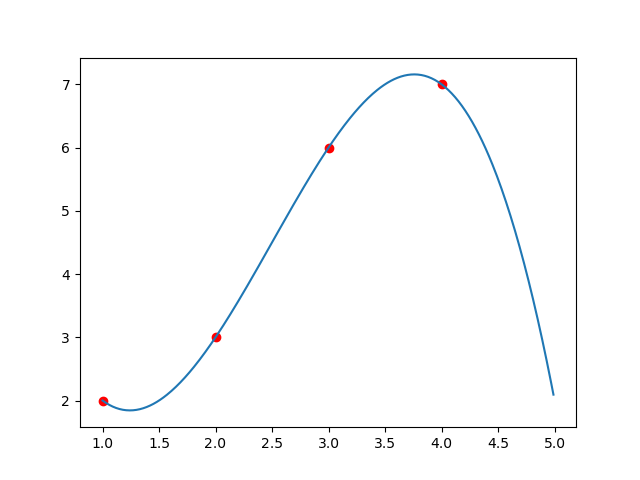
\includegraphics[width=1\linewidth]{Chapter2/graph/python/Figure2-1.png}
    \caption{Lagrange多项式插值(使用上述代码生成)}
    \label{fig:Lagrange多项式插值}
\end{figure}
    \chapter{函数逼近与计算}

\section{引言}

\subsection{函数逼近的问题的一般提法}

对于函数类$A$中给定的函数$f(x)$, 要求在另一类较简单且便于计算的函数类$B(\subset A)$中寻找一个函数$P(x)$, 使得函数$P(x)$与$f(x)$之差在某种度量意义下最小.

本章所研究的函数类$A$通常为区间$[a,b]$上的连续函数, 记作$C[a,b]$; 函数类$B$通常为\emph{代数多项式}或三角多项式.

\subsection{常用的度量标准}

\subsubsection{最佳一致逼近}

\begin{definition}[最佳一致逼近]
    若以函数$f(x)$和$P(x)$的最大误差
    \begin{equation*}
        \max_{x\in[a,b]}\abs{f(x)-P(x)}=\norm{f(x)-P(x)}_\infty
    \end{equation*}
    作为度量误差$f(x)-P(x)$"大小"的标准, 在这种意义下的函数逼近称为\emph{最佳一致逼近}或\emph{均匀逼近}
\end{definition}

\subsubsection{最佳平方逼近}

\begin{definition}[最佳平方逼近]
    采用
    \begin{equation*}
        \sqrt{\int_a^b\left[f(x)-P(x)\right]^2\dd{x}}=\norm{f(x)-P(x)}_2
    \end{equation*}
    作为度量误差"大小"标准的函数逼近称为\emph{最佳平方逼近}或\emph{均方逼近}.
\end{definition}

\section{最佳一致逼近}

\subsection{最佳一致逼近概念}

\begin{definition}
    设函数$f(x)$是区间$[a,b]$上的连续函数, 对于任意给定的$\varepsilon>0$, 如果存在多项式$P(x)$, 使不等式
    \begin{equation*}
        \max_{a\le x\le b}\abs{f(x)-P(x)}<\varepsilon
    \end{equation*}
    成立, 则称多项式$P(x)$在区间$[a,b]$上\emph{一致逼近}(或\emph{均匀逼近})于函数$f(x)$.
\end{definition}

\subsection{最佳一致逼近多项式的存在性}

\begin{theorem}[Weierstrass定理]
    若$f(x)$是区间$[a,b]$上的连续函数, 则对于任意$\varepsilon>0$, 总存在多项式$P(x)$, 使对一切$a\le x\le b$, 有
    \begin{equation*}
        \norm{f(x)-P(x)}_\infty<\varepsilon
    \end{equation*}
\end{theorem}

定理证明略. % 未证明

可以证明的是, 多项式$P(x)$形式为:
\begin{equation*}
    P(x)=\sum_{i=0}^{n(\varepsilon)}f\left(\frac{i}{n}\right)C_n^ix^i(1-x)^{n-i}
\end{equation*}
且
\begin{equation*}
    \lim\limits_{n\to\infty}P_n(x)\to f(x)
\end{equation*}

\subsection{$C[a,b]$上最佳一致逼近}

在次数不超过$n$的多项式当中, 找到一个$p_n^*(x)$, 使得
\begin{equation*}
    \norm{f(x)-p_n^*(x)}_\infty=\min_{p_n(x)\in H_n}\norm{f(x)-p_n(x)}_\infty
\end{equation*}
其中, $H_n$表示由所有次数不超过$n$的代数多项式构成的线性空间. 上述问题为$C[a,b]$空间中最佳一致逼近问题.

下面的定理说明了该最佳一致逼近多项式的存在性.

\begin{theorem}[Borel定理]
    对任意的$f(x)\in C[a,b]$, 在$H_n$中都存在对$f(x)$的最佳一致逼近多项式, 记为$p_n^*(x)$, 使得
    \begin{equation*}
        \norm{f(x)-p_n^*(x)}_\infty=\min_{p_n(x)\in H_n}\norm{f(x)-p_n(x)}_\infty
    \end{equation*}
    称$p_n^*(x)$为$f(x)$的\emph{n次最佳一致逼近多项式}. 或简称为\emph{最佳逼近多项式}.
\end{theorem}

\subsection{相关概念}

\subsubsection{偏差}

\begin{definition}[偏差]
    若$P_n(x)\in H_n, f(x)\in C[a,b]$, 则称
    \begin{equation*}
        \Delta(f,P_n)=\norm*{f-P_n}_\infty=\max_{a\le x\le b}\abs*{f(x)-P_n(x)}
    \end{equation*}
    为$f(x)$与$P_n(x)$在$[a,b]$上的\emph{偏差}
\end{definition}

显然, $\Delta(f,P_n)\le 0$, ${\Delta(f,P_n)}$的全体组成一个集合, 记作$\Delta(f,H_n)$, 下界为0.

\subsubsection{最小偏差}

\begin{definition}
    若记集合的下确界为
    \begin{equation*}
        E_n=\inf_{P_n\in H_n}\left\{\Delta(f,P_n)\right\}=\inf_{P_n\in H_n}\max_{a\le x\le b}\abs*{f(x)-P_n(x)}
    \end{equation*}
    则称$E_n$为$f(x)$在$[a,b]$上的\emph{最小偏差}
\end{definition}

\subsubsection{偏差点}

\begin{definition}[偏差点]
    设$f(x)\in C[a,b], P(x)\in H_n$, 若在$x=x_0$上有
    \begin{equation*}
        \abs*{P(x_0)-f(x_0)}=\max_{a\le x\le b}\abs*{P(x)-f(x)}=\mu
    \end{equation*}
    则称$x_0$是$P(x)-f(x)$的\emph{偏差点}.

    若$P(x_0)-f(x_0)=\mu$, 则称$x_0$为\emph{正偏差点};

    若$P(x_0)-f(x_0)=-\mu$, 则称$x_0$为\emph{负偏差点};
\end{definition}

\subsubsection{交错点组}

\begin{definition}
    若函数$f(x)$在其定义域内的某一区间$[a,b]$上存在$n$个点${x_k},k=1,2,\cdots,n$, 使得
    \begin{align*}
        \abs*{f(x_k)}&=\max\abs*{f(x)}=\norm*{f(x)}_\infty, k=1,2,\cdots,n\\
        -f(x_k)&=f(x_{k+1}), k=1,2,\cdots,n-1
    \end{align*}
    则称点集${x_k},k=1,2,\cdots,n$为函数$f(x)$在区间$[a,b]$上的一个\emph{交错点组}, 点$x_k$为\emph{交错点}.
\end{definition}

\subsection{$C[a,b]$上的最佳一致逼近特征}

\begin{lemma}
    设$f(x)$是区间$[a,b]$上的连续函数, $P_n^*(x)$是$f(x)$的$n$次最佳一致逼近多项式, 则$f(x)-P_n^*(x)$在区间$[a,b]$上必同时存在正负偏差点.
\end{lemma}

\begin{theorem}[Chebyshev定理]
    设$f(x)$是区间$[a,b]$上的连续函数, 则$P_n^*(x)$是$f(x)$的$n$次最佳一致逼近多项式的充要条件是:$f(x)-P_n^*(x)$在区间$[a,b]$上存在一个至少由$n+2$个点组成的交错点组.
\end{theorem}

\begin{example}
    求函数$f(x)=\sin{4x}$在$[0,2\pi]$上的6次最佳一致逼近$P_6^*(x)$
\end{example}

\begin{solution}
    令
    \begin{equation*}
        R(x)=f(x)-P_6^*(x)
    \end{equation*}
    考虑函数$f(x)=\sin{4x}$在区间$[0,2\pi]$存在由8个点组成的交错点组.

    令$R(x)=\sin{4x}$, 则有
    \begin{equation*}
        P_6^*(x)=f(x)-R(x)=0
    \end{equation*}
\end{solution}

\begin{corollary}
    在$P_n[a,b]$中, 若存在对函数$f(x)\in C[a,b]$的最佳一致逼近元, 则唯一.
\end{corollary}

\begin{corollary}
    设$f(x)$是区间$[a,b]$上的连续函数, 则$f(x)$的$n$次最佳一致逼近多项式是$f(x)$的某个$n$次插值多项式.
\end{corollary}

\begin{corollary}
    设$f(x)$是区间$[a,b]$上的连续函数, $P_n^*(x)$是$f(x)$的$n$次最佳一致逼近多项式, 若$f^{(n+1)}(x)$在$(a,b)$内存在且保号, 则$f(x)-P_n^*(x)$在区间$[a,b]$上恰好存在一个由$n+2$个点组成的交错点组, 且两个端点$a,b$都在交错点组中.
\end{corollary}

\subsection{一次最佳逼近多项式($n=1$)}

\subsubsection{推导过程}

设$f(x)\in C^2[a,b]$, 且$f''(x)$在$(a,b)$内不变号, 要求$f(x)$在$[a,b]$上的一次最佳一致逼近多项式$P_1(x)=a_0+a_1x$. 由上述推论, $f(x)-P_1(x)$在$[a,b]$上恰好由3个点构成的交错点组, 且区间端点$a,b$属于交错点组. 设另一交错点组为$x_2$. 则有
\begin{equation*}
    \begin{cases}
        f'(x_2)-P_1'(x_2)=0\\
        f(a)-P_1(a)=f(b)-P_1(b)\\
        f(a)-P_1(a)=-\left[f(x_2)-P_1(x_2)\right]
    \end{cases}
\end{equation*}
即
\begin{equation*}
    \begin{cases}
        f'(x_2)=a_1\\
        a_0+a_1a-f(a)=f(x_2)-[a_0+a_1x_2]\\
        a_0+a_1a-f(a)=a_0+a_1b-f(b)
    \end{cases}
\end{equation*}

解得
\begin{align*}
    a_1&=\frac{f(b)-f(a)}{b-a}=f'(x_2)\\
    a_0&=\frac{f(a)+f(x_2)}{2}-\frac{f(b)-f(a)}{b-a}\frac{a+x_2}{2}
\end{align*}
即
\begin{equation*}
    P_1(x)=\frac{f(x_2)+f(a)}{2}+\frac{f(b)-f(a)}{b-a}\left(x-\frac{a+x_2}{2}\right)
\end{equation*}

\begin{example}
    求R$f(x)=\sqrt{1+x^2}$在$[0,1]$上的一次最佳一致逼近多项式.
\end{example}
\begin{solution}
    因为
    \begin{align*}
        f'(x)&=\frac{x}{\sqrt{1+x^2}}\\
        f''(x)&=\frac{1}{\sqrt[3]{(1+x^2)^2}}>0
    \end{align*}
    设$f(x)$在$[0,1]$上的一次最佳一致逼近多项式为$P_1(x)=a_0+a_1x$, 则由
    \begin{equation*}
        a_1=\frac{f(b)-f(a)}{b-a}=f'(x_2)
    \end{equation*}
    可得
    \begin{equation*}
        a_1=\sqrt{2}-1\approx0.414
    \end{equation*}

    再由
    \begin{equation*}
        f'(x_2)=a_1
    \end{equation*}
    可得
    \begin{equation*}
        \frac{x_2}{\sqrt{1+x_2^2}}=\sqrt{2}-1
    \end{equation*}
    解得
    \begin{equation*}
        x_2=\sqrt{\frac{\sqrt{2}-1}{2}}\approx0.4551, f(x_2)=\sqrt{1+x_2^2}\approx1.0986
    \end{equation*}
    由
    \begin{equation*}
        a_0=\frac{f(a)+f(x_2)}{2}-\frac{f(b)-f(a)}{b-a}\frac{a+x_2}{2}
    \end{equation*}
    得
    \begin{equation*}
        a_0=\frac{1+\sqrt{1+x_2^2}}{2}-a_1\frac{x_2}{2}\approx0.955
    \end{equation*}
    于是得$\sqrt{1+x^2}$得最佳一次逼近多项式为
    \begin{equation*}
        P_1(x)=0.955+0.414x
    \end{equation*}

    最小偏差为
    \begin{equation*}
        \norm*{\sqrt{1+x^2}-P_1(x)}_\infty=\max_{0\le x\le1}\abs*{\sqrt{1+x^2}-P_1(x)}=\abs*{\sqrt{1+0^2}-P_1(0)}\le0.045
    \end{equation*}
\end{solution}

\subsubsection{$n$次最佳一致逼近多项式(推广)}

设$f(x)\in C^{n+1}[a,b]$, 且$f^{(n+1)}(x)$在$(a,b)$内不变号吗要求$f(x)$在$[a,b]$上得$n$次最佳一致逼近多项式
\begin{equation*}
    P_n(x)=a_0+a_1x+\cdots+a_nx^n
\end{equation*}

由推论可知, $f(x)-P_n(x)$在$[a,b]$上恰好有$n+2$个点构成得交错点组, 且$a,b$属于交错点组. 设另外$n$个交错点为$x_1,x_2,\cdots,x_n$, 则有
\begin{equation*}
    \begin{cases}
        f'(x_i)-P_n'(x_i)=0, i=1,2,\cdots,n\\
        f(a)-P_n(a)=(-1)^i(f(x_i)-P_n(x_i)), i=1,2,\cdots,n\\
        f(a)-P_n(a)=(-1)^{n+1}\left[f(b)-P_n(b)\right]
    \end{cases}
\end{equation*}

\subsection{Chebyshev多项式及其应用}

\subsubsection{定义}

\begin{definition}[Chebyshev多项式]
    称
    \begin{equation*}
        T_n=\cos(n\arccos{x}), \abs*{x}\le 1
    \end{equation*}
    为Chebyshev多项式
\end{definition}

注: 令$\theta=\arccos{x}$, 则$\cos\theta=x$. 而
\begin{equation*}
    \cos{n\theta}=\cos^n{\theta}-C_n^2\cos^{n-2}{\theta}\sin^2\theta+C_n^4\cos^{n-4}\theta\sin^4\theta-\cdots
\end{equation*}
故$T_n$是关于$x$得$n$次代数多项式.

\subsubsection{性质}

正交性: 由$T_n(x)$所组成的序列${T_n(x)}$在区间$[-1,1]$上带权$\rho(x)=\frac{1}{\sqrt{1-x^2}}$的正交多项式序列, 且
\begin{equation*}
    \int_{-1}^1\frac{1}{\sqrt{1-x^2}}T_m(x)T_n(x)\dd{x}=
    \begin{cases}
        0,&m\ne n\\
        \frac{\pi}{2},&m=n\ne0\\
        \pi,&m=n=0
    \end{cases}
\end{equation*}

递推关系: 相邻的三个Chebyshev多项式具有如下递推关系式:
\begin{equation*}
    \begin{cases}
        T_0(x)=1, T_1(x)=x\\
        T_{n+1}(x)=2x\cdot T_n(x)-T_{n-1}(x), n=1,2,\cdots
    \end{cases}
\end{equation*}

奇偶性: Chebyshev多项式$T_n$, 当$n$为奇数时为奇函数, 当$n$为偶数时为偶函数. 即
\begin{align*}
    T_n(-x)&=\cos[n\arccos(-x)]=\cos(n\pi-n\arccos{x})\\
    &=(-1)^n\cos(n\arccos{x})=(-1)^nT_n(x)
\end{align*}

$T_n$在区间$[-1,1]$上有$n$个不同的零点
\begin{equation*}
    x_k=\cos{\frac{(2k-1)\pi}{2n}}, k=1,2,\cdots,n
\end{equation*}

$T_n(x)$在$[-1,1]$上有$n+1$个不同的极值点
\begin{equation*}
    x_k'=\cos{k\frac{\pi}{n}}, k=0,1,\cdots,n
\end{equation*}
使$T_n(x)$轮流取得最大值1和最小值-1.

$T_n(x)$的最高次项系数为$2^{n-1}, n=1,2,\cdots$

在区间$[-1,1]$上, 在所有首项系数为1的$n$次多项式$p_n(x)$中. $\widetilde{T}_n(x)=\frac{1}{2^{n-1}}T_n(x)$与零的偏差最小, 且偏差为$\frac{1}{2^{n-1}}$, 即对于任何$p(x)\in H_n(x)$, 有
\begin{equation*}
    \frac{1}{2^{n-1}}=\norm*{\widetilde{T}_n(x)-0}_\infty=\min_{p(x)\in H_n}\norm*{p(x)-0}_\infty
\end{equation*}

上述性质又被称为Chebyshev多项式的\emph{最小模性质}.

\subsubsection{应用}

设$f(x)=b_0+b_1x+\cdots+b_{n+1}x^{n+1}(b_{n+1}\ne0)$为$[-1,1]$上的$n+1$次多项式, 要求$f(x)$在$[-1,1]$上的$n$次最佳一致逼近$P_n^*(x)$.

由于首项系数为1的$n+1$次Chebyshev多项式$\widetilde{T}_{n+1}(x)$无穷范数最小, 有
\begin{equation*}
    \frac{f(x)-P_n^*(x)}{b_{n+1}}=\widetilde{T}_{n+1}(x)=\frac{1}{2^n}T_{n+1}(x)
\end{equation*}
于是
\begin{equation*}
    P_n^*(x)=f(x)-b_{n+1}\widetilde{T}_{n+1}(x)
\end{equation*}
其偏差为
\begin{equation*}
    \norm*{f(x)-P_n^*(x)}_\infty=\norm*{\frac{b_{n+1}}{2^n}T_{n+1}(x)}_\infty=\frac{\abs*{b_{n+1}}}{2^n}
\end{equation*}

\begin{example}
    设$f(x)=4x^4+2x^3-5x^2+8x-\frac{5}{2}, \abs*{x}\le 1$, 求$f(x)$在$[-1,1]$上的3次最佳一致逼近元$P_3^*(x)$
\end{example}
\begin{solution}
    由$f(x)$的表达式可知$b_4=4$, 首项系数为1的4次Chebyshev多项式为
    \begin{equation*}
        \widetilde{T}_4(x)=x^4-x^2+\frac{1}{8}
    \end{equation*}
    设$f(x)$在$[-1,1]$上的3次最佳一致逼近多项式为$P_3^*(x)$, 则
    \begin{equation*}
        \frac{f(x)-P_3^*(x)}{4}=\widetilde{T}_4(x)
    \end{equation*}
    从而
    \begin{equation*}
        P_3^*(x)=f(x)-4\widetilde{T}_4(x)=2x^3-x^2+8x-3
    \end{equation*}
    其最小偏差为
    \begin{equation*}
        \norm*{f(x)-P_3^*(x)}_\infty=\norm*{\frac{b_4}{2^3}T_4(x)}_\infty=\frac{\abs*{4}}{2^3}=\frac{1}{2}
    \end{equation*}
\end{solution}

\begin{example}
    若$f(x)=4x^4-5x^2+8x-\frac{5}{2}, \abs*{x}\le 1$, 重求上题
\end{example}
\begin{solution}
    重复上述步骤, 可得3次最佳一致逼近多项式为
    \begin{equation*}
        P_3^*(x)=-x^2+8x-3
    \end{equation*}

    (注意: 这里的3次多项式是次数不超过3)
\end{solution}

考虑一般区间$[a,b]$上的多项式降阶. 设$f(x)=b_0+b_1x+\cdots+b_{n+1}x^{n+1}, b_{n+1}\ne 0$为$[a,b]$上的$n+1$次多项式, 要求$f(x)$在$[a,b]$上的$n$次最佳一致逼近$P_n^*(x)$.

首先做区间变换, 令
\begin{equation*}
    x=\frac{b-a}{2}t+\frac{b+a}{2}
\end{equation*}
其中$t\in[-1,1]$, 则
\begin{equation*}
    f(x)=f\left(\frac{b-a}{2}t+\frac{b+a}{2}\right)=g(t)\in C[-1,1]
\end{equation*}

设$g(t)$在$[-1,1]$的$n$次最佳一致逼近多项式为$P_n(t)$, 则
\begin{equation*}
    P_n(t)=g(t)-c_{n+1}\widetilde{T}_{n+1}(t)
\end{equation*}
其中, $c_{n+1}$为$g(t)$的最高此项系数.
\begin{equation*}
    c_{n+1}=b_{n+1}\left(\frac{b-a}{2}\right)^{n+1}
\end{equation*}
于是, $f(x)$在$[a,b]$上的$n$次最佳一致逼近多项式为
\begin{equation*}
    P_n^*(x)=P_n\left(\frac{2x-b-a}{b-a}\right)
\end{equation*}
最小偏差为
\begin{equation*}
    \norm*{f(x)-P_n(x)}_\infty=\norm*{g(t)-P_n(t)}_\infty=\frac{\abs*{c_{n+1}}}{2^n}
\end{equation*}

下面再考虑插值多项式的情况. 设$f(x)\in C[-1,1]$, 且存在$n+1$阶连续导数$f^{(n+1)}(x)$. 如何在$[-1,1]$上确定互异节点$x_0,x_1,\cdots,x_n$, 使得$f(x)$的$n$次插值多项式的余项最小.

由插值余项定理, 可知$n$次插值多项式$L_n(x)$的余项为
\begin{equation*}
    R_n(x)=f(x)-L_n(x)=\frac{f^{(n+1)}(\xi)}{(n+1)!}\omega_{n+1}(x)
\end{equation*}
其中, 
\begin{equation*}
    \omega_{n+1}(x)=\prod_{i=0}^n(x-x_i), \xi\in(-1,1)
\end{equation*}
其误差上界为
\begin{align*}
    \abs*{f(x)-L_n(x)}&\le\frac{1}{(n+1)!}\max_{-1\le x\le1}\abs*{f^{(n+1)}(x)}\max_{-1\le x\le1}\abs*{\omega_{n+1}(x)}\\
    &=\frac{1}{(n+1)!}\norm*{f^{(n+1)}}_\infty\norm*{\omega_{n+1}(x)}_\infty
\end{align*}

要使余项达到最小, 即令$\norm*{\omega_{n+1}(x)}_\infty$尽可能小. 由于是一个首项系数为1的$n+1$次多项式. 故有Chebyshev多项式, 取
\begin{equation*}
    \omega_{n+1}(x)=\widetilde{T}_{n+1}(x)
\end{equation*}
同时有
\begin{equation*}
    \omega_{n+1}(x)=\prod_{i=0}^n(x-x_i)
\end{equation*}
故只需令$x_i,i=0,1,\cdots,n$为$n+1$次Chebyshev多项式的零点, 即
\begin{equation*}
    x_i=\cos\frac{(2i+1)\pi}{2(n+1)}, i=0,1,\cdots,n
\end{equation*}

\section{最佳平方逼近}

\subsection{内积空间}

\subsubsection{内积空间定义}

\begin{definition}[内积空间]
    设$X$为(实)线性空间, 在$X$上定义了内积是指对$X$中每一对元素$x,y$, 都有一实数, 记为$(x,y)$与之对应, 且这个对应满足:
    \begin{enumerate}
        \item \begin{equation*}
            (x,x)\ge0, (x,x)=0\Leftrightarrow x=0
        \end{equation*};
        \item \begin{equation*}
            (x,y)=(y,x),x,y\in X
        \end{equation*};
        \item \begin{equation*}
            (\lambda x,y)=\lambda(x,y), x,y\in X; \lambda\in R
        \end{equation*};
        \item \begin{equation*}
            (x+y,z)=(x,z)+(y,z), x,y,z\in X
        \end{equation*}
    \end{enumerate}
    则称$X$为\emph{内积空间}, 称二元函数$(x,y)$为\emph{内积}
\end{definition}

\subsubsection{2-范数定义及其性质}

\begin{definition}
    设$X$为内积空间, 则对任意的$x\in X$, 称
    \begin{equation*}
        \norm*{x}_2=\sqrt{(x,x)}
    \end{equation*}
    为$x$的\emph{2-范数}或\emph{欧式范数}.

    特别的, 对$f(x)\in C[a,b]$, 称
    \begin{equation*}
        \norm*{f}_2=\sqrt{\int_a^b\rho(x)f^2(x)\dd{x}}=\sqrt{(f,f)}
    \end{equation*}
    为函数$f(x)$的\emph{Euclid范数}
\end{definition}

设$X$是一内积空间, 则对任意的$x,y\in X$, 有
\begin{enumerate}
    \item Cauchy-Schwarz不等式:
    \begin{equation*}
        (x,y)^2\le(x,x)(y,y)
    \end{equation*}
    \item 三角不等式:
    \begin{equation*}
        \norm*{x+y}_2\le\norm*{x}_2+\norm*{y}_2
    \end{equation*}
\end{enumerate}

讨论特殊的两种内积空间, 
\begin{itemize}
    \item $n$维欧氏空间$R^n$, 内积就是两向量数量积, 即
    \begin{equation*}
        (x,y)=x^Ty=\sum x_iy_i
    \end{equation*}
    \item 连续函数空间$C[a,b]$, 内积定义为积分运算或带权函数积分运算, 即
    \begin{equation*}
        (f(x),g(x))=\int_a^bf(x)g(x)\dd{x}, f(x),g(x)\in C[a,b]
    \end{equation*}
    或者
    \begin{equation*}
        (f(x),g(x))=\int_a^b\rho(x)f(x)g(x)\dd{x}, f(x),g(x)\in C[a,b]
    \end{equation*}
\end{itemize}

\begin{definition}[权函数]
    设$\rho(x)$定义在有限或无限区间$[a,b]$上, 如果具有下列性质:
    \begin{enumerate}
        \item 对任意$x\in [a,b], \rho(x)\ge 0$;
        \item 积分$\int_a^b\abs*{x}^n\rho(x)\dd{x}$存在, $n=0,1,2,\cdots$;
        \item 对非负的连续函数$g(x)$, 若$\int_a^bg(x)\rho(x)\dd{x}=0$, 则在$(a,b)$上有$g(x)\equiv0$
    \end{enumerate}
    称满足上述条件的 $\rho(x)$为$[a,b]$上的\emph{权函数}
\end{definition}

\subsection{相关概念}

\subsubsection{距离}

$R^n$中, 两个向量$x,y$之间的距离定义为
\begin{equation*}
    \text{dist}(x,y)=\norm*{x-y}_2=\sqrt{(x-y,x-y)}=\sqrt{\sum_i(x_i-y_i)^2}
\end{equation*}

连续函数空间$C[a,b]$中, 两个函数$f(x)$与$g(x)$的欧式距离为
\begin{equation*}
    \text{dist}(f(x),g(x))=\norm*{f(x)-g(x)}_2=\sqrt{\int_a^b\rho(x)\left[f(x)-g(x)\right]^2\dd{x}}
\end{equation*}

\subsubsection{正交}

在$R^n$中, 若两个向量$x,y$的内积为零, 即
\begin{equation*}
    (x,y)=0
\end{equation*}
则称向量$x,y$\emph{正交}.

在连续函数空间$C[a,b]$中, 若函数$f(x)$与$g(x)$满足
\begin{equation*}
    (f,g)=\int_a^b\rho(x)f(x)g(x)\dd{x}=0
\end{equation*}
则称$f(x)$与$g(x)$在$[a,b]$上\emph{带权$\rho(x)$正交}.

进一步, 设在$C[a,b]$上给定函数系${\varphi_k(x)}$, 若满足条件
\begin{equation*}
    (\varphi_j(x),\varphi_k(x))=\begin{cases}
        0,&j\ne k\\
        \text{常数}A_k>0,&j=k, j,k=0,1,\cdots
    \end{cases}
\end{equation*}
则称函数系${\varphi_k(x)}$是$[a,b]$上带权$\rho(x)$的正交坐标系.

特别地, 若$A_k=1$, 则该函数系称为\emph{标准正交坐标系}.

若上述定义中函数系为多项式系, 则称之为$C[a,b]$上带权$\rho(x)$的\emph{正交多项式系}, 并称$\varphi_n(x)$为$[a,b]$上带权$\rho(x)$的\emph{$n$次正交多项式}.

\subsection{内积空间上的最佳平方逼近}

\subsubsection{函数系的线性关系}

\begin{definition}
    设$\varphi_0(x),\varphi_1(x),\cdots,\varphi_n(x)$为区间$[a,b]$上的连续函数, 若关系式
    \begin{equation*}
        a_0\varphi_0(x)+a_1\varphi_1(x)+\cdots+a_n\varphi_n(x)=0
    \end{equation*}
    当且仅当$a_0=a_1=\cdots=a_n=0$时成立, 则称函数在$[a,b]$上是\emph{线性无关}的, 否则称\emph{线性相关}.
\end{definition}

\subsubsection{函数系线性无关的判别条件}

\begin{theorem} % 待证明
    连续函数$\varphi_0(x),\varphi_1(x)\cdots,\varphi_n(x)$在$[a,b]$上线性无关的充分必要条件是它们的Gram行列式
    \begin{equation*}
        G_n=
        \mqty|(\varphi_0,\varphi_0)&(\varphi_0,\varphi_1)&\cdots&(\varphi_0,\varphi_n)\\
        (\varphi_1,\varphi_0)&(\varphi_1,\varphi_1)&\cdots&(\varphi_1,\varphi_n)\\
        \vdots&\vdots&\cdots&\vdots\\
        (\varphi_n,\varphi_0)&(\varphi_n,\varphi_1)&\cdots&(\varphi_n,\varphi_n)|\ne 0
        \end{equation*}
\end{theorem}

设$\varphi_0(x),\varphi_1(x),\cdots,\varphi_n(x)$是$[a,b]$上线性无关的连续函数, $a_0,a_1,\cdots,a_n$是任意实数, 则
\begin{equation*}
    S(x)=a_0\varphi_0(x)+a_1\varphi_1(x)+\cdots+a_n\varphi_n(x)
\end{equation*}
的全体是$C[a,b]$的一个子集, 记作
\begin{equation*}
    \Phi=\spn{\varphi_0,\varphi_1,\cdots,\varphi_n}
\end{equation*}
并称$\varphi_0(x),\varphi_1(x),\cdots,\varphi_n(x)$是生成集合$\Phi$的一个基底.

\subsubsection{最佳平方逼近元的定义}

设$X$为线性内积空间, $\varphi_0,\varphi_1,\cdots,\varphi_n$为$X$上$n+1$个线性无关元, 即
\begin{equation*}
    \Phi=\spn{\varphi_0,\varphi_1,\cdots,\varphi_n}
\end{equation*}

\begin{definition}[最佳平方逼近元]
    对任意的$X\in X$, 在$X$的子空间$\Phi$中, 求$g$的在2-范数意义下的最佳逼近元$S^*$, 即求$S^*\in\Phi$, 使得
    \begin{equation*}
        \norm*{S^*-g}_2=\min_{S\in\Phi}\norm*{S-g}_2
    \end{equation*}
    对任意$S\in\Phi$成立. 若满足上式的$S^*\in\Phi$存在, 则称$S^*$为$g\in X$的\emph{最佳平方逼近元}
\end{definition}

\subsubsection{最佳平方逼近元的存在性}

\begin{theorem}%待证明
    设$X$为线性内积空间, 由线性无关组$\varphi_0,\varphi_1,\cdots,\varphi_n$张成的线性空间$\Phi$为$X$的子空间, 则对任意的$g\in X$, 存在$S^*\in \Phi$为$g$的最佳平方逼近元.
\end{theorem}

\subsubsection{最佳平方逼近元的特征}

\begin{theorem} % 待证明
    $S^*\in\Phi=\spn{\varphi_0,\varphi_1,\cdots,\varphi_n}$为$g\in X$(线性内积空间)的最佳平方逼近元的充要条件是: $g-S^*$与一切${\varphi_j},j=0,1,\cdots,n$正交. 其中, $\varphi_0,\varphi_1,\cdots,\varphi_n$为$X$的$n+1$个线性无关元.
\end{theorem}

该定理所说的$g-S^*$与一切$\varphi_j$正交, 指$g-S^*$与一切$\varphi_j$的内积为零, 即
\begin{equation*}
    (g-S^*,\varphi_j)=0, j=0,1,\cdots,n
\end{equation*}

\subsubsection{最佳平方逼近元的唯一性}

\begin{theorem}
    线性内积空间$X$的子空间$\Phi$中若存在对$g\in X$的最佳平方逼近元, 则唯一.
\end{theorem}

\subsubsection{最佳平方逼近元的求解}

由最佳平方逼近元充要条件, 若假定
\begin{equation*}
    S^*=\sum_{j=0}^nc_j^*\varphi_j(x)
\end{equation*}
则可得出
\begin{equation*}
    \left(g-\sum_{j=0}^nc_j^*\varphi_j,\varphi_i\right)=0, i=0,1,\cdots,n
\end{equation*}
移项变形为
\begin{equation*}
    \left(\sum_{j=0}^nc_j^*\varphi_j,\varphi_i\right)=(\varphi_i,g), i=0,1,\cdots,n
\end{equation*}
其中, $c_j^*,j=0,1,\cdots,n$为待定系数. 用矩阵表示方程组为:
\begin{equation*}
    \mqty(
        (\varphi_0,\varphi_0)&(\varphi_0,\varphi_1)&\cdots&(\varphi_0,\varphi_n)\\
        (\varphi_1,\varphi_0)&(\varphi_1,\varphi_1)&\cdots&(\varphi_1,\varphi_n)\\
        \vdots&\vdots&\cdots&\vdots\\
        (\varphi_n,\varphi_0)&(\varphi_n,\varphi_1)&\cdots&(\varphi_n,\varphi_n)
    )\mqty(
        c_0^*\\c_1^*\\\vdots\\c_n^*
    )=\mqty(
        (\varphi_0,g)\\(\varphi_1,g)\\\vdots\\(\varphi_n,g)
    )
\end{equation*}
此方程称为\emph{法方程组}.

若选取的一组基底${\varphi_0(x),\varphi_1(x),\cdots,\varphi_n(x)}$满足
\begin{equation*}
    (\varphi_i,\varphi_j)=\begin{cases}
        0,&i\ne j\\
        A_i>0,&i=j
    \end{cases}
\end{equation*}
则称其为\emph{正交基}, 此时
\begin{equation*}
    c_j^*=\frac{(\varphi_j,g)}{(\varphi_j,\varphi_j)}, j=0,1,\cdots,n
\end{equation*}

\subsubsection{最佳平方逼近元的误差估计}

设$S^*=\sum_{j=0}^nc_j^*\varphi_j\in\Phi=\spn{\varphi_0,\varphi_1,\cdots,\varphi_n}$为$g\in X$的最佳平方逼近元, 则其平方误差为
\begin{align*}
    \norm*{g-S^*}_2^2&=(g-S^*,g-S^*)=(g-S^*,g)-(g-S^*,S^*)\\
    &=(g-S^*,g)-(g-S^*,\sum_{j=0}^nc_j^*\varphi_j)\\
    &=(g,g)-(S^*,g)-\sum_{j=0}^nc_j^*(g-S^*,\varphi_j)\\
    &=(g,g)-(S^*,g)=(g,g)-\sum_{j=1}^nc_j^*(g-\varphi_j)
\end{align*}

均方误差为
\begin{equation*}
    \norm*{g-S^*}_2=\sqrt{(g,g)-\sum_{j=0}^nc_j^*(g,\varphi_j)}
\end{equation*}

\subsection{连续函数的最佳平方逼近}

对于给定的函数$f(x)\in C[a,b]$, 要求函数
\begin{equation*}
    S^*\in\Phi=\spn{\varphi_0,\varphi_1,\cdots,\varphi_n}
\end{equation*}
使
\begin{equation*}
    \int_a^b\rho(x)\left[f(x)-S^*(x)\right]^2\dd{x}=\min_{S(x)\in\Phi}\int_a^b\rho(x)\left[f(x)-S(x)\right]^2\dd{x}
\end{equation*}

若这样的$S^*(x)$存在, 则称为$f(x)$在区间$[a,b]$上的\emph{最佳平方逼近函数}.

特别地, 若取$\Phi=H_n=\spn{1,x,\cdots,x^n}$, 则称
\begin{equation*}
    S^*(x)=a_0\cdot1+a_1x+\cdots+a_nx^n
\end{equation*}
为$f(x)$在$[a,b]$上的\emph{$n$次最佳平方逼近多项式}.

计算$C[a,b]$上函数$f(x)$的$n$次最佳平方逼近多项式. 取
\begin{equation*}
    \varphi_0=1, \varphi_1=x,\cdots,\varphi_n=x^n
\end{equation*}
设$f(x)$的$n$次最佳平方逼近多项式为
\begin{equation*}
    S^*(x)=\sum_{j=0}^na_j\cdot\varphi_j(x)=\sum_{j=0}^na_j\cdot x^j
\end{equation*}
构造法方程组:
\begin{equation*}
    \mqty(
        (\varphi_0,\varphi_0)&(\varphi_0,\varphi_1)&\cdots&(\varphi_0,\varphi_n)\\
        (\varphi_1,\varphi_0)&(\varphi_1,\varphi_1)&\cdots&(\varphi_1,\varphi_n)\\
        \vdots&\vdots& &\vdots\\
        (\varphi_n,\varphi_0)&(\varphi_n,\varphi_1)&\cdots&(\varphi_n,\varphi_n)\\
    )\mqty(
        a_0\\a_1\\\vdots\\a_n
    )=\mqty(
        (f,\varphi_0)\\(f,\varphi_1)\\\vdots\\(f,\varphi_0)
    )
\end{equation*}
其中, 
\begin{align*}
    (\varphi_i,\varphi_j)&=\int_a^b\varphi_i\cdot\varphi_j\dd{x}=\int_a^bx^i\cdot x^j\dd{x}\\
    &=\frac{b^{i+j+1}-a^{i+j+1}}{i+j+1}, i,j=0,1,\cdots,n
\end{align*}
\begin{equation*}
    (f,\varphi_j)=\int_a^bf(x)\cdot\varphi_j\dd{x}=\int_a^bf(x)\cdot x^j\dd{x}, j=0,1,\cdots,n
\end{equation*}
由此可得函数$f(x)$在$H_n$中的$n$次最佳平方逼近多项式:
\begin{equation*}
    S^*(x)=\sum_{j=0}^na_j^*x^j
\end{equation*}
平方误差为:
\begin{equation*}
    \norm*{f(x)-S^*(x)}_2^2=(f,f)-\sum_{j=0}^na_j^*(f,\varphi_j)=\int_a^b\left[f(x)\right]^2\dd{x}-\sum_{j=0}^na_j^*(f,\varphi_j)
\end{equation*}

由于$\varphi_0,\varphi_1,\cdots,\varphi_n$线性无关, 故$G_n\ne 0$, 上述方程组存在唯一解$a_k=a_k^*, k=0,1,\cdots,n$

特别地, 当$a=0,b=1$时, 法方程组系数矩阵为
\begin{equation*}
    H=\mqty(
        1&\frac{1}{2}&\frac{1}{3}&\cdots&\frac{1}{n+1}\\
        \frac{1}{2}&\frac{1}{3}&\frac{1}{4}&\cdots&\frac{1}{n+2}\\
        \frac{1}{3}&\frac{1}{4}&\frac{1}{5}&\cdots&\frac{1}{n+3}\\
        \vdots&\vdots&\vdots& &\vdots\\
        \frac{1}{n+1}&\frac{1}{n+2}&\frac{1}{n+3}&\cdots&\frac{1}{2n+1}\\
    )
\end{equation*}
该矩阵为Hilbert矩阵, 为病态矩阵.

\begin{example}
    求$g(x)=\sqrt{x}$在$H_1[0,1]$中的最佳平方逼近元, 并估计误差
\end{example}

\begin{solution}
    取$\varphi_0=1,\varphi_1=x, H_1[0,1]=\spn{1,x}$, 记
    \begin{equation*}
        S_1^*(x)=a_0+a_1x
    \end{equation*}
    由
    \begin{align*}
        (\varphi_0,\varphi_0)&=\int_0^11\cdot1\dd{x}=1\\
        (\varphi_0,\varphi_1)&=\int_0^11\cdot x\dd{x}=\frac{1}{2}\\
        (\varphi_1,\varphi_1)&=\int_0^1x\cdot x\dd{x}=\frac{1}{3}
    \end{align*}
    同样可求得
    \begin{align*}
        (\varphi_0,g)&=\int_0^1\sqrt{x}\dd{x}=\frac{2}{3}\\
        (\varphi_1,g)&=x\cdot\sqrt{x}\dd{x}=\frac{2}{5}
    \end{align*}

    所以, 关于$a_0,a_1$的法方程组为
    \begin{equation*}
        \begin{cases}
            a_0+\frac{1}{2}a_1=\frac{2}{3}\\
            \frac{1}{2}a_0+\frac{1}{3}a_1=\frac{2}{5}
        \end{cases}
    \end{equation*}
    解得
    \begin{equation*}
        a_0=\frac{4}{15}, a_1=\frac{4}{5}
    \end{equation*}
    即$S_1^*(x)=\frac{4}{5}x+\frac{4}{155}$为$H_1[0,1]$对$g(x)$的最佳平方逼近元. 且误差为
    \begin{align*}
        \norm*{\delta_n}_2^2&=\norm*{\sqrt{x}-S_1^*(x)}_2^2=\int_0^1\left(\sqrt{X}\right)^2\dd{x}-\sum_{k=0}^1a_k\left(\sqrt{k}.\varphi_k\right)\\
        &=\frac{1}{2}-\frac{4}{15}\cross\frac{2}{3}-\frac{4}{5}\cross\frac{2}{5}=\frac{1}{255}\approx0.0044
    \end{align*}
\end{solution}

\section{正交多项式}

\subsection{正交化手续}

当权函数$\rho(x)$及区间$[a,b]$给定后, 可由幂函数系${1,x,x^2,\cdots,x^n,\cdots}$利用Schmidt正交化方法构造出和正交多项式系
\begin{align*}
    g_0(x)&=1,\\
    g_k(x)&=x^k-\sum_{i=0}^{k-1}\frac{(x^k,g_i)}{(g_i,g_i)}\cdot g_i, k=1,2,\cdots
\end{align*}

\subsection{正交多项式的性质}

\begin{enumerate}
    \item $g_n(x)$是最高次项系数为1的$n$次多项式.
    \item 任一$n$次多项式 $P_n(x)\in H_n$均可表示为$g_0(x),g_1(x),\cdots,g_n(x)$的线性组合.
    \item 当$n\ne m$ 时, $(g_n,g_m)=0$, 且$g_n(x)$与任一次数小于$n$的多项式正交.
    \item 递推性, 
    \begin{equation*}
        g_{n+1}(x)=(x-\alpha_n)g_n(x)-\beta_ng_{n-1}(x), n=0,1,\cdots
    \end{equation*}
    其中, 
    \begin{align*}
        g_0(x)&=1, g_{-1}(x)=0,\\
        \alpha_n&=\frac{(xg_n,g_n)}{(g_n,g_n)}, n=0,1,\cdots,\\
        \beta_n&=\frac{(g_n,g_n)}{(g_{n-1},g_{n-1})}, n=1,2,\cdots
    \end{align*}
    这里$(xg_n,g_n)=\int_a^bxg_n^2(x)\rho(x)\dd{x}$
    \item 设$g_0(x),g_1(x),\cdots$是在$[a,b]$上带权$\rho(x)$的正交多项式序列, 则$g_n(x)(n\ge1)$的$n$个根都是单重实根, 且都在区间$(a,b)$内.
\end{enumerate}

\subsection{常用的正交多项式}

\subsubsection{第一类Chebyshev多项式}

定义:
\begin{equation*}
    T_n=\cos\left(n\arccos{x}\right),\abs*{x}\le 1
\end{equation*}

性质:

\begin{enumerate}
    \item 递推关系
    \begin{equation*}
        \begin{cases}
            T_0(x)=1, T_1(x)=x\\
            T_{n+1}(x)=2x\cdot T_n(x)-T_{n-1}(x), n=1,2,\cdots
        \end{cases}
    \end{equation*}

    \item 正交性
    
    由$T_n(x)$所组成的序列${T_n(x)}$在区间$[-1,1]$上带权$\rho(x)=\frac{1}{\sqrt{1-x^2}}$的正交多项式序列, 且
    \begin{equation*}
        (T_m(x),T_n(x))=\int_{-1}^1\frac{1}{\sqrt{1-x^2}}T_m(x)T_n(x)\dd{x}=
        \begin{cases}
            0,&m\ne n\\
            \frac{\pi}{2},&m=n\ne 0\\
            \pi,&m=n=0
        \end{cases}
    \end{equation*}
\end{enumerate}

\subsubsection{Legendre多项式}

\begin{definition}[$n$次Legendre多项式]
    多项式
    \begin{equation*}
        P_n(x)=\frac{1}{2^n\cdot n!}\dv[n]{x}\left[(x^2-1)^n\right], n=0,1,2,\cdots
    \end{equation*}
    称为\emph{$n$次Legendre多项式}
\end{definition}

正交性: Legendre多项式序列${P_n(x)}$是$[-1,1]$上带权$\rho=1$的正交多项式序列, 且
\begin{equation*}
    (P_m(x),P_n(x))=\int_{-1}^1P_m(x)P_n(x)\dd{x}=
    \begin{cases}
        0,&m\ne n\\
        \frac{2}{2n+1},& m=n
    \end{cases}
\end{equation*}

相邻的三个Legendre多项式具有如下递推关系:
\begin{equation*}
    \begin{cases}
        P_0(x)=1, P_1(x)=x,
        P_{n+1}(x)=\frac{2x+1}{n+1}xP_n(x)-\frac{n}{n+1}P_{n-1}(x), n=1,2,\cdots
    \end{cases}
\end{equation*}

奇偶性: 当$n$为偶数时, $P_n(x)$为偶函数; 当$n$为奇数时, $P_n(x)$为奇函数.

$P_n(x)$在区间$[-1,1]$内存在$n$个互异实零点. 且最高项系数为$\frac{(2n)!}{2^n(n!)^2}$

在所有首项系数为1的$n$次多项式中, Legendre多项式$\widetilde{P}_n(x)$在$[-1,1]$上与零的平方误差最小. 即对于任何$p(x)\in H_n(x)$, 有
\begin{equation*}
    \norm*{\widetilde{P}_n(x)-0}_2=\min_{p(x)\in H_n}\norm*{p(x)-0}_2
\end{equation*}

\begin{extend}
    \begin{equation*}
        \norm*{\widetilde{T}_n(x)-0}_\infty=\min_{p(x)\in H_n}\norm*{p(x)-0}_\infty
    \end{equation*}
\end{extend}

\subsubsection{其他常用的正交多项式}

\begin{definition}[第二类Chebyshev多项式]
    称
    \begin{equation*}
        U_n(x)=\frac{\sin\left[(n+1)\arccos{x}\right]}{\sqrt{1-x^2}}
    \end{equation*}
    为第二类Chebyshev多项式
\end{definition}

其中, ${U_n(x)}$是区间$[-1,1]$带权$\rho(x)=\sqrt{1-x^2}$的正交多项式序列,
\begin{equation*}
    \int_{-1}^1\sqrt{1-x^2}U_m(x)U_n(x)\dd{x}=
    \begin{cases}
        0,&m\ne n\\
        \frac{\pi}{2},&m=n
    \end{cases}
\end{equation*}

且具有如下递推关系式:
\begin{equation*}
    \begin{cases}
        U_0(x)=1, U_1(x)=2x\\
        U_{n+1}(x)=2xU_n(x)-U_{n-1}(x), n=1,2,\cdots
    \end{cases}
\end{equation*}

\begin{definition}[Laguerre多项式]
    称多项式
    \begin{equation*}
        L_n(x)=e^x\dv[n]{x}(x^ne^{-x}), 0\le x<+\infty, n=0,1,2,\cdots
    \end{equation*}
    为Laguerre多项式
\end{definition}

${L_n(x)}$是定义在区间$[0,+\infty)$上带权$\rho(x)=e^{-x}$的正交多项式序列.
\begin{equation*}
    \int_0^\infty e^{-x}\cdot L_m(x)L_n(x)\dd{x}=
    \begin{cases}
        0,&m\ne n\\
        (n!)^2,& m=n
    \end{cases}
\end{equation*}

递推关系式:
\begin{equation*}
    \begin{cases}
        L_0(x)=1, L_1(x)=1-x\\
        L_{n+1}(x)=(1+2n-x)L_n(x)-n^2\cdot L_{n-1}(x), n=1,2,\cdots
    \end{cases}
\end{equation*}

\begin{definition}[Hermite多项式]
    称多项式
    \begin{equation*}
        H_n(x)=(-1)^n\cdot e^{x^2}\cdot\dv[n]{x}(e^{-x^2}), x\in(-\infty, \infty), n=0,1,2,\cdots
    \end{equation*}
    为Hermite多项式
\end{definition}

${H_n(x)}$是区间$(-\infty, \infty)$上带权$\rho(x)=e^{-x^2}$的正交多项式序列.
\begin{equation*}
    \int_{-\infty}^\infty e^{-x^2}H_m(x)\cdot H_n(x)\dd{x}=
    \begin{cases}
        0, &m\ne n\\
        2^n\cdot n!\cdot\sqrt{\pi},& m=n
    \end{cases}
\end{equation*}

递推关系式
\begin{equation*}
    \begin{cases}
        H_0(x)=1, H_1(x)=2x\\
        H_{n+1}(x)=2xH_n(x)-2nH_{n-1}(x), n=1,2,\cdots
    \end{cases}
\end{equation*}

\section{函数按正交多项式展开}

设$\Phi=\spn{\varphi_0,\varphi_1,\cdots,\varphi_n}$, 其中$\varphi_i(i=0,1,\cdots,n)$是$[a,b]$上带权$\rho(x)$的正交多项式系, 给定$f(x)\in C[a,b]$, 若$S_n^*(x)=a_0\varphi_0(x)+\cdots+a_n\varphi_n(x)$为$f(x)$在$[a,b]$上的$n$次最佳平方逼近多项式, 则由正交多项式的性质
\begin{equation*}
    a_k=\frac{(f,\varphi_k)}{(\varphi_k,\varphi_k)}, k=0,1,\cdots,n
\end{equation*}
于是
\begin{equation*}
    S_n^*(x)=\sum_{k=0}^n\frac{(f,\varphi_k)}{(\varphi_k,\varphi_k)}\varphi_k(x)
\end{equation*}
其均方误差为
\begin{equation*}
    \norm*{\delta_n}_2=\norm*{f(x)-S_n^*(x)}_2=\sqrt{(f,f)-\sum_{k=0}^n a_k^2(\varphi_k,\varphi_k)}
\end{equation*}

\begin{example}
    求$f(x)=e^x$在$[-1,1]$上的三次最佳平方逼近多项式.
\end{example}

\begin{solution}
    考虑使用Legendre多项式, 计算$(f,P_k),k=0,1,2,3$, 即
    \begin{align*}
        (f,P_0)&=\int_{-1}^1e^x\dd{x}=e-\frac{1}{e}\approx2.3504\\
        (f,P_1)&=\int_{-1}^1xe^x\dd{x}=2e^{-1}\approx0.7358\\
        (f,P_2)&=\int_{-1}^1\left(\frac{3}{2}x^2-\frac{1}{2}\right)e^x\dd{x}=e-\frac{7}{e}\approx0.1431\\
        (f,P_3)&=\int_{-1}^1\left(\frac{5}{2}x^3-\frac{3}{2}x\right)e^x\dd{x}=\frac{37}{e}-5e\approx0.2013
    \end{align*}

    所以得
    \begin{align*}
        a_0^*&=\frac{(f,P_0)}{2}=1.1752\\
        a_1^*&=3\frac{(f,P_1)}{2}=1.1036\\
        a_2^*&=5\frac{(f,P_2)}{2}=0.3578\\
        a_3^*&=7\frac{(f,P_3)}{2}=0.07046
    \end{align*}
    
    所以
    \begin{align*}
        S_3^*(x)&=1.1752+1.1036x+0.3578\left(\frac{3}{2}x^2-\frac{1}{2}\right)+0.07046\left(\frac{5}{2}x^3-\frac{3}{2}x\right)\\
        &=0.9963+0.9979x+0.5367x^2+0.1761x^3
    \end{align*}

    均方误差为
    \begin{equation*}
        \norm*{\delta_n}_2=\norm*{e^x-S_3^*(x)}_2=\sqrt{\int_{-1}^1e^{2x}\dd{x}-\sum_{k=0}^3\frac{2}{2k+1}a_k^{*2}}\le0.0084
    \end{equation*}

    最大误差为
    \begin{equation*}
        \norm*{\delta_n}_\infty=\norm*{e^x-S_3^*(x)}_\infty\le0.0112
    \end{equation*}
\end{solution}

下面使用Python代码演示这道题. 注意, 代码当中的系数为Legendre多项式的系数.

\begin{lstlisting}
# 使用Legendre多项式进行平方逼近演示(例题解答) Exercise3-1.py
import numpy as np
from scipy.special import legendre
from scipy.optimize import least_squares

# 计算Legendre多项式的系数
def legendre_coefficients(x, y, degree):
    A = np.zeros((len(x), degree + 1))
    for i in range(degree + 1):
        A[:, i] = legendre(i)(x)
    return np.linalg.lstsq(A, y, rcond=None)[0]
# 定义逼近函数
def approximation_func(x, coefficients):
    result = np.zeros_like(x)
    for i, coeff in enumerate(coefficients):
        result += coeff * legendre(i)(x)
    return result
def legendre_approximation(x, y, degree):
    # 计算逼近函数的系数
    coefficients = legendre_coefficients(x, y, degree)
    # 使用最小二乘法优化逼近函数的系数
    result = least_squares(lambda coefficients: approximation_func(x, coefficients) - y, coefficients)
    return result.x

x = np.linspace(-1, 1, 100)
y = np.exp(x)
# 最佳平方逼近
degree = 3
coefficients = legendre_approximation(x, y, degree)
# 计算逼近函数的值
approximation = approximation_func(x, coefficients)
# 打印结果
print("系数:", coefficients)
\end{lstlisting}

输出结果为:[1.17530022 1.10367036 0.35831431 0.07053157], 与计算结果一致.

\section{曲线拟合的最小二乘法}

\subsection{问题提出}

已知一系列测量数据$(x_i,y_i)$, 要求简单函数$f(x)$使得$\rho_i=y_i-f(x_i)$在总体上尽可能小. 这里$y_i\ne f(x_i)$, 称$\rho_i$为\emph{残差}, 这种构造近似函数的方法称为\emph{曲线拟合}, $f(x)$为\emph{拟合函数}.

通常, 使$\rho_i$尽可能小的度量准则包括:

\begin{itemize}
    \item 使$\max_{1\le ile m}\abs*{P(x_i)-y_i}$尽可能小;
    \item 使$\sum_{i=1}^m\abs*{P(x_i)-y_i}$尽可能小;
    \item 使$\sum_{i=1}^m\abs*{P(x_i)-y_i}^2$尽可能小
\end{itemize}

\subsection{曲线拟合的步骤}

\begin{enumerate}
    \item 根据条件画出散点图;
    \item 观察分布, 选择适当的函数类构造拟合函数;
    \item 根据某一逼近准则确定拟合函数的未知参数.
\end{enumerate}

\subsection{2-范数度量下的曲线拟合(最小二乘法)}

给定一组数据$(x_i,y_i), i=1,2,\cdots,m$, 确定拟合函数
\begin{equation*}
    f(x)=c_1\varphi_1(x)+c_2\varphi_2(x)+\cdots+c_n\varphi_n(x)
\end{equation*}
使得
\begin{equation*}
    \norm*{r}_2^2=\sum_{i=1}^m\rho_i^2=\sum_{i=1}^m\left[y_i-f(x_i)\right]^2=\sum+{i-1}^m\left[y_i-\sum_{j=1}^nc_j\varphi_j(x_i)\right]^2
\end{equation*}
达到极小, 这里$n\le m$.

若记
\begin{equation*}
    E(c_1,c_2,\cdots,c_n)=\sum_{i=1}^m\left[y_i-\sum_{j=1}^nc_j\varphi_j(x_i)\right]^2
\end{equation*}
则$E$是$c_1,\cdots,c_n$的多元函数, 于是问题转化为求多元函数$E(c_1,c_2,\cdots,c_n)$的极小值问题.

由多元函数极值必要条件, 在$E$的极值点处, 有
\begin{equation*}
    \pdv{E}{c_k}=\sum_{i=1}^m-2\left(y_i-\sum_{j=1}^nc_j\varphi_k(x_i)\right)\varphi_k(x_i)=0, k=1,2,\cdots,n
\end{equation*}
即
\begin{equation*}
    \sum_{j=1}^nc_j\sum_{i=1}^m\varphi_j(x_i)\varphi_k(x_i)=\sum_{i=1}^my_i\varphi_k(x_i), k=1,2,\cdots,n
\end{equation*}

若记
\begin{equation*}
    \Phi_i=\mqty(
        \varphi_i(x_1)\\\varphi_i(x_2)\\\vdots\\\varphi_i(x_m)
    ), i=1,2,\cdots,n,b=\mqty(
        y_1\\y_2\\\vdots\\y_m
    )
\end{equation*}
则
\begin{align*}
    \sum_{i=1}^m\varphi_j(x_i)\varphi_k(x_i)&=(\Phi_j,\Phi_k)
    \sum_{i=1}^my_i\varphi_k(x_i)=(\Phi_k,b)
\end{align*}
于是上式可写为
\begin{equation*}
    \sum_{j=1}^nc_j(\Phi_j,\Phi_k)=(\Phi_k,b), k=1,2,\cdots,n
\end{equation*}
于是有关于$c_1,c_2,\cdots,c_n$的线性方程组
\begin{equation*}
    \mqty(
        (\Phi_1,\Phi_1)&(\Phi_2,\Phi_1)&\cdots&(\Phi_n,\Phi_1)\\
        (\Phi_1,\Phi_2)&(\Phi_2,\Phi_2)&\cdots&(\Phi_n,\Phi_2)\\
        \vdots&\vdots&&\vdots\\
        (\Phi_1,\Phi_n)&(\Phi_2,\Phi_n)&\cdots&(\Phi_n,\Phi_n)\\
    )\mqty(
        c_1\\c_2\\\vdots\\c_n
    )=\mqty(
        (\Phi_1,b)\\(\Phi_2,b)\\\vdots\\(\Phi_n,b)
    )
\end{equation*}
或等价写作:
\begin{equation*}
    \mqty(
        \Phi_1^T\Phi_1&\Phi_2^T\Phi_1&\cdots&\Phi_n^T\Phi_1\\
        \Phi_1^T\Phi_2&\Phi_2^T\Phi_2&\cdots&\Phi_n^T\Phi_2\\
        \vdots&\vdots& &\vdots\\
        \Phi_1^T\Phi_n&\Phi_2^T\Phi_n&\cdots&\Phi_n^T\Phi_n
    )\mqty(
        c_1\\c_2\\\vdots\\v_n
    )=\mqty(
        \Phi_1^T\\\Phi_2^T\\\vdots\\\Phi_n^T
    )b
\end{equation*}

若记
\begin{align*}
    A&=(\Phi_1,\Phi_2,\cdots,\Phi_n)=\mqty(
        \varphi_1(x_1)&\varphi_2(x_1)&\cdots&\varphi_n(x_1)\\
        \varphi_1(x_2)&\varphi_2(x_2)&\cdots&\varphi_n(x_2)\\
        \vdots&\vdots& &\vdots\\
        \varphi_1(x_m)&\varphi_2(x_m)&\cdots&\varphi_n(x_m)\\
    )\\
    x&=\mqty(
        c_1\\c_2\\\vdots\\c_n
    )
\end{align*}
则上述方程组可表示为
\begin{equation*}
    A^TAx=A^Tb
\end{equation*}
由于$A$是列满秩矩阵(列向量线性无关), 故系数矩阵对称正定, 方程组的解存在唯一, 故可得拟合参数$c_1,c_2,\cdots,c_n$

\begin{extend}
    若矩阵$A\in\mathbb{R}^{m\cross n}$, 则$A^TA\in\mathbb{R}^{n\cross n}, AA^T\in\mathbb{R}^{m\cross m}$, 它们具有如下共同特点:
    
    \begin{itemize}
        \item 对称半正定($\forall x\in\mathbb{R}^n, x^T(A^TA)x\ge 0$);
        \item 特征值非负;
        \item $\rank(A^TA)=\rank(AA^T)=\rank(A)$;
        \item 非零特征值个数相同, 且非零特征值相同;
        \item $\tr(AA_T)=\tr(A^TA)$
    \end{itemize}
\end{extend}

若取$\varphi_0=1,\varphi_1(x)=x,\varphi_2(x)=x^2,\cdots,\varphi_n(x)=x^n$, 则拟合函数
\begin{equation*}
    f(x)=c_0+c_1x+c_2x^2+\cdots+c_nx^n
\end{equation*}
称为\emph{多项式拟合}, 此时
\begin{align*}
    A&=\mqty(
        1&x_1&x_1^2&\cdots&x_1^n\\
        1&x_2&x_2^2&\cdots&x_2^n\\
        \vdots&\vdots&\vdots& &\vdots\\
        1&x_m&x_m^2&\cdots&x_m^n\\
    )\\
    b&=\mqty(y_1\\y_2\\\vdots\\y_m)\\
    x&=\mqty(c_0\\c_1\\\vdots\\c_n)
\end{align*}
于是
\begin{equation*}
    A^TAx=A^Tb
\end{equation*}

一些特殊情况下的非线性拟合, 可通过变量代换, 转换为线性拟合. 例如:
\begin{enumerate}
    \item 双曲拟合
    \begin{equation*}
        \frac{1}{y}=a+b\frac{1}{x}\Rightarrow u=a+bv(u=\frac{1}{y},v=\frac{1}{x})
    \end{equation*}
    \item 对数拟合
    \begin{equation*}
        y=a+b\ln{x}\Rightarrow y=a+bu(u=\ln{x})
    \end{equation*}
    \item 指数拟合
    \begin{equation*}
        y=ae^{bx}\Rightarrow\ln{y}=\ln{a}+bx\Rightarrow u=c+bx(u=\ln{y},c=\ln{a})
    \end{equation*}
\end{enumerate}

\subsection{用正交函数作最小二乘拟合}

给定
\begin{equation*}
    \begin{cases}
        x_0,\cdots,x_m\\
        y_0,\cdots,y_m
    \end{cases}
\end{equation*}
与正交函数系$\varphi_0,\varphi_1,\cdots,\varphi_n$, 则最小二乘拟合系数为:
\begin{equation*}
    P_n(x)=a_0\varphi_0(x)+a_1\varphi_1(x)+\cdots+a_n\varphi_n(x)
\end{equation*}
其中,
\begin{equation*}
    a_k=\frac{(f,\varphi_k)}{(\varphi_k,\varphi_k)}=\frac{\sum_{i=0}^m\rho(x_i)y_i\varphi_k(x_i)}{\sum_{i=1}^m\rho(x_i)\varphi_k^2(x_i)}
\end{equation*}

最后以一个最小二乘法的例题结束这一章.

\begin{example}
    给定$(t_i,f_i)$的一组数据

    \begin{tabular}{|c|c|}
        \hline
        $t_i$&$f_i$\\
        \hline
        0&81.4\\
        20&77.7\\
        40&74.2\\
        60&72.4\\
        80&70.3\\
        100&68.8\\
        \hline
    \end{tabular}

    求拟合函数$f(x)$
\end{example}

\begin{solution}
    作图可知点分布在直线附近, 故使用线性函数拟合. 设
    \begin{equation*}
        \varphi_0(t)=1, \varphi_1(t)=t
    \end{equation*}
    将数据代入, 可得
    \begin{equation*}
        A=\mqty(
            1&0\\
            1&20\\
            1&40\\
            1&60\\
            1&80\\
            1&100
        ), x=\mqty(c_1\\c_2), b=\mqty(
            81.4\\77.7\\74.2\\72.4\\70.3\\68.8
        )
    \end{equation*}
    代入公式
    \begin{equation*}
        A^TAx=A^Tb
    \end{equation*}
    可得拟合函数为
    \begin{equation*}
        f(t)=80.3-0.1t
    \end{equation*}
\end{solution}

下面的代码实现了上面的计算功能:
\begin{lstlisting}
# 演示线性拟合的最小二乘法 Exercise3-2.py
import numpy as np
import matplotlib.pyplot as plt
# 数据
x = np.array([0,20,40,60,80,100])
y = np.array([81.4,77.7,74.2,72.4,70.3,68.8])
# 进行线性拟合
coefficients = np.polyfit(x, y, 1)
slope = coefficients[0]
intercept = coefficients[1]
# 绘制拟合曲线
x_fit= np.arange(0,100,0.01)
y_fit = slope*x_fit+intercept
plt.scatter(x,y)
plt.plot(x_fit,y_fit,c="red")
plt.show()
# 打印拟合结果
print(f"表达式为{slope:.1f}t+{intercept:.1f}")
\end{lstlisting}

拟合结果图像如图\ref{fig:使用线性拟合结果}所示.

\begin{figure}[h]
    \centering
    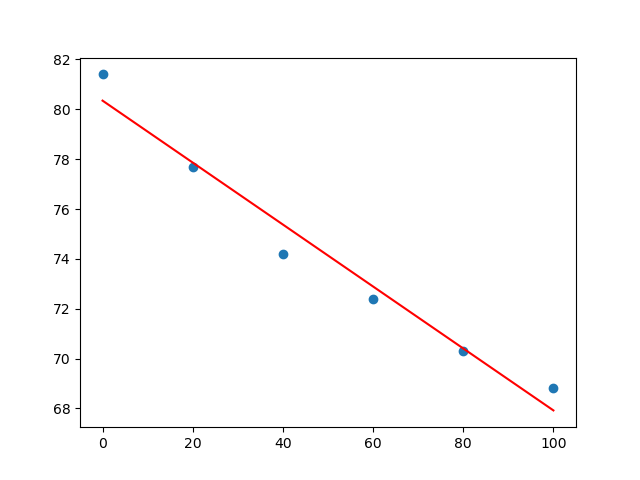
\includegraphics[width=1\linewidth]{Chapter3/graph/python/Figure3-1.png}
    \caption{使用线性拟合结果}
    \label{fig:使用线性拟合结果}
\end{figure}

最后作为扩展演示, 下面是一个使用Legendre多项式进行三次拟合的程序:

\begin{lstlisting}
# 使用Legendre多项式进行三次拟合 Exercise3-3.py
import numpy as np
import matplotlib.pyplot as plt
from scipy.special import legendre
# 示例数据
x = np.array([3.73,5.63,8.67,10.49,13.26,16.74,
19.55,22.19,25.36,28.31,30.83])
y = np.array([21.53,21.43,21.43,21.33,21.22,
20.71,20.20,19.69,18.78,17.76,16.84])
# 进行Legendre拟合
coefficients = np.polynomial.legendre.legfit(x, y, 3)
# 绘制拟合曲线
x_fit = np.arange(3.73,30.83,0.01)
y_fit = np.polynomial.legendre.legval(x_fit, coefficients)
plt.scatter(x,y)
plt.plot(x_fit,y_fit,c="red")
plt.show()
\end{lstlisting}

得到图像如图\ref{fig:使用Legendre多项式进行三次拟合}所示.

\begin{figure}[h]
    \centering
    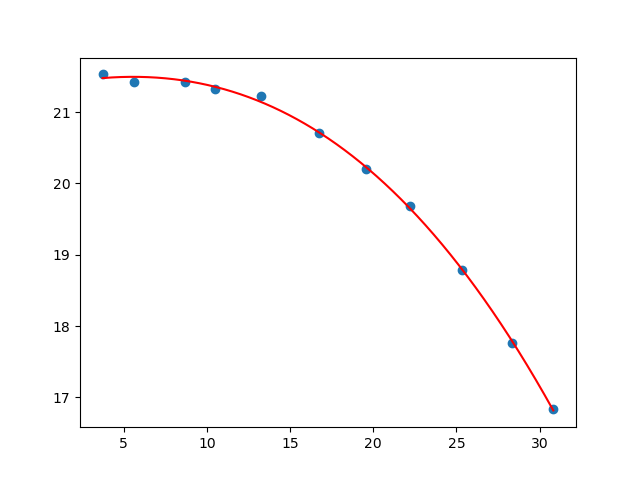
\includegraphics[width=1\linewidth]{Chapter3/graph/python/Figure3-2.png}
    \caption{使用Legendre多项式对一组数据进行三次拟合}
    \label{fig:使用Legendre多项式进行三次拟合}
\end{figure}
    \chapter{数值积分}

\section{引言}

\subsection{数值积分的必要性}
本章主要讨论如下形式的一元函数积分
\begin{equation*}
    I(f) = \int_{a}^{b}f(x)\dd{x}
\end{equation*}
在微积分里, 按Newton-Leibniz公式求定积分
\begin{equation*}
    I(f) = \int_{a}^{b}f(x)\dd{x} = F(b)-F(a)
\end{equation*}

要求$f(x)$的原函数$F(x)$:
\begin{itemize}
    \item 有解析表达式;
    \item 为初等函数.
\end{itemize}

实际上,
\begin{enumerate}
    \item $f(x)$的原函数$F(x)$不能用初等函数表示,如$\sin{x^2},\cos{x^2},\frac{\sin{x}}{x},\frac{1}{\ln{x}}$等;
    \item 被积函数的原函数可以用初等函数表示,但其表达式相当复杂,计算极不方便,如$x^2\sqrt{2x^2+3}$;
    \item $f(x)$没有表达式,只有数表形式。
\end{enumerate}
这时就需要积分的数值方法来帮忙了。

\subsection{数值积分的基本思想}
\subsubsection{数值积分的理论依据}
依据积分中值定理,对于连续函数$f(x)$,在$[a,b]$内存在一点$\xi $,使得
    \begin{equation*}
       I(f) = \int_{a}^{b}f(x)\dd{x} = (b-a)f(\xi )
    \end{equation*}
称$f(\xi )$为$f(x)$在区间$[a,b]$上的平均高度。

\subsubsection{求积公式的构造}

 若简单选取区间端点或中点的函数值作为平均高度,则求积公式(左矩形公式, 中矩形公式, 右矩形公式)如下:
    \begin{equation*}
        I(f)\approx f(a)(b-a)
    \end{equation*}
    \begin{equation*}
        I(f)\approx f(\frac{a+b}{2})(b-a)
    \end{equation*}
    \begin{equation*}
        I(f)\approx f(b)(b-a)
    \end{equation*}

\begin{definition}[两点求积公式]
    若取$a,b$两点,并令$f(\xi ) = \frac{f(a)+f(b)}{2}$,则可得到梯形公式(两点求积公式)
    \begin{equation*}
        I(f)\approx \frac{f(a)+f(b)}{2}(b-a)
    \end{equation*}
\end{definition}

\begin{definition}[三点求积公式/Simpson公式]
    若取三点,$a,b,c = \frac{a+b}{2}$并令$f(\xi ) = \frac{[f(a)+4f(c)+f(b)]}{6}$,则可得Simpson公式(三点求积公式)
    \begin{equation*}
        I(f)\approx (b-a)\frac{[f(a)+4f(c)+f(b)]}{6}
    \end{equation*}  
\end{definition}

\begin{definition}[机械求积]
    一般地,取区间$[a,b]$内$n+1$个点${x_i},(i=0,1,2,\cdots,n)$处的高度${f(x_i)},(i=0,1,2,\cdots,n)$,通过加权平均的方法近似地得出平均高度$f(\xi )$。这类求积方法称为机械求积。
    \begin{equation*}
        \int_{a}^{b}f(x)\dd{x} \approx (b-a)\sum_{i=0}^{n}\lambda_if(x_i)
    \end{equation*}
    或写成:
    \begin{equation*}
        \int_{a}^{b}f(x)\dd{x} \approx \sum_{k=0}^{n}A_kf(x_k)
    \end{equation*}
    其中$A_k$称为求积系数,$x_k$称为求积节点。
\end{definition}

记:

数值求积公式:
\begin{equation*}
     i_n(f) = \sum_{k=0}^{n}A_kf(x_k)   
\end{equation*}

求积公式余项(误差):
\begin{equation*}
    R(f) = I(f)-I_n(f) = \int_{a}^{b}f(x)\dd{x}-\sum_{k=0}^{n} A_kf(x_k)
\end{equation*}

构造或确定一个求积公式,要解决的问题包括:
\begin{enumerate}
    \item 确定求积系数$A_k$和求积节点$x_k$;
    \item 确定衡量求积公式好坏的标准;
    \item 求积公式的误差估计和收敛性分析.
\end{enumerate}

\subsection{求积公式的代数精度}

\begin{definition}
    称求积公式$I_n(f)=\sum_{k=0}^{n}A_kf(x_k)$具有$m$次代数精度,如果它满足如下两个条件:
    \begin{enumerate}
        \item 对所有$m$次多项式$P_m(x)$,有
        \begin{equation*}
            R(P_m) = I(P_m)-I_n(P_m) = 0
        \end{equation*}
        \item 存在$m+1$次多项式$P_{m+1}(x)$,使得
        \begin{equation*}
            R(P_{m+1}) = I(P_{m+1})-I_n(P_{m+1}) \ne 0
        \end{equation*}
    \end{enumerate}
    上述定义中的条件等价于:
    \begin{align*}
         R(x^k) &= I(x^k)-I_n(x^k) = 0,(0\leq k\leq m)\\
         R(x_{m+1})&\neq 0
    \end{align*}
    \begin{notice}
        梯形公式与中矩形公式都只具有1次代数精度。
    \end{notice}
\end{definition}



一般的,若要使求积公式(1)具有m次代数精度, 则只要使求积公式对$f(x) = 1,x,x^2,\cdots,x^m$都准确成立,即
\begin{equation*}
    \begin{cases}
        \sum_{k=0}^{n}A_k = b-a\\
        \sum_{k=0}^{n}A_kx_k = \frac{1}{2}(b^2-a^2)\\
        \sum_{k=0}^{n}A_kx^m_k = \frac{1}{m+1}(b^{m+1}-a^{m+1})
    \end{cases}
\end{equation*}

\section{插值型求积公式}

\subsection{定义}

\begin{definition}[拉格朗日插值公式]
    在积分区间$[a,b]$上,取$n+1$个节点$x_i,i=0,1,2,\cdots,n$作$f(x)$的$n$次代数插值多项式(拉格朗日插值公式):
    \begin{equation*}
        L_n(x) = \sum_{k=0}^{n}l_k(x)f(x_k)
    \end{equation*}
    则有$f(x) = L_n(x)+R_n(x)$
    其中,$R_n(x) = \frac{f^{(n+1)}(\xi)}{(n+1)!}w_{n+1}(x)$为插值余项。
    $w_{n+1}(x) = \prod_{j=0}^{n}(x-x_j)$
\end{definition}

于是有:
\begin{align*}
    \int_{a}^{b}f(x)\dd{x} &= \int_{a}^{b}L_n(x)\dd{x}+\int_{a}^{b}R_n(x)\dd{x} \\
    &= \sum_{j=0}^{n}[\int_{a}^{b}l_j(x)\dd{x}]f(x_j)+\int_{a}^{b}R_n(x)\dd{x}
\end{align*}
取
\begin{equation*}
    \int_{a}^{b}f(x)\dd{x} \approx \sum_{j=0}^{n}f(x_j)\int_{a}^{b}l_i(x)\dd{x}
\end{equation*}
其中$\int_{a}^{b} l_j(x)\dd{x}$为$A_j$。

$A_j = \int_{a}^{b} \prod_{i=0,i\neq j}^{n}\frac{(x-x_i)}{(x_j-x_i)}\dd{x}$由节点决定,与$f(x)$无关。


\subsection{截断误差与代数精度}

\subsubsection{截断误差}
\begin{align*}
    R(f) &= \int_{a}^{b}f(x)\dd{x} - \sum_{k=0}^{n}A_kf(x_k) \\
    &= \int_{a}^{b}[f(x)-L_n(x)]\dd{x} \\
    &= \int_{a}^{b}\frac{f^{n+1}(\xi_x)}{(n+1)!}\prod_{k=0}^{n}(x-x_k)\dd{x}
\end{align*}

\subsubsection{代数精度}
\begin{theorem}
    形如$\sum_{k=0}^{n}A_kf(x)$的求积公式至少有$n$次代数精度$\Leftrightarrow $该公式为插值型(即:$A_k = \int_{a}^{b}l_k(x)dx$)
    \begin{corollary}
        求积系数$A_k$满足:
        \begin{equation*}
            \sum_{k=0}^{n}A_k = b-a
        \end{equation*}
    \end{corollary}
\end{theorem}

\section{Newton-Cotes公式}

\subsection{Cotes系数}
取节点为等距分布:$x_i=a+ih, h=\frac{b-a}{n}, i=0,1,\cdots,n$
由此构造的插值型求积公式称为Newton-Cotes公式,此时
求积系数:
\begin{align*}%令$x=a+th$
    A_i &= \int_{x_0}^{x_n}\prod_{j\neq i}\frac{(x-x_j)}{x_i-x_j}\dd{x} \\
    &=\int_{0}^{n}\prod_{i\neq j}\frac{(t-j)h}{(i-j)h}\times h\dd{t} \\
    &= \frac{(b-a)(-1)^{n-i}}{ni!(n-i)!}\int_{0}^{n}\prod_{j\neq i}(t-j)\dd{t}\\
    &= C_i^{(n)}(b-a)
\end{align*}
其中,$C_i^{(n)}$为Cotes系数。

\subsection{Newton-Cotes公式}

\subsubsection{定义}

\begin{definition}[n阶闭型Newton-Cotes求积公式]
    记:
    \begin{equation*}
        C_i^{(n)} = \frac{(-1)^{n-i}}{i!(n-i)!n}\int_{0}^{n}[\prod_{k=0, k\neq i}^{n}(t-k)]\dd{t}
    \end{equation*}
    则$A_i = (b-a)C_i^{(n)},i=0,1,2,\cdots,n$
    求积公式变为
    \begin{equation*}
        \int_{a}^{b}f(x)\dd{x} \approx (b-a)\sum_{i=0}^{n}C_i^{(n)}f(x_i)
    \end{equation*}
    称上式为n阶闭型Newton-Cotes求积公式。
\end{definition}

\begin{notice}
    由式$C_i^{(n)} = \frac{(-1)^{n-i}}{i!(n-i)!n}\int_{0}^{n}[\prod_{k=0,k\neq i}^{n}(t-k)]\dd{t}$确定的Cotes系数只与$i$和$n$有关,与$f(x)$和积分区间$[a,b]$无关,且满足:
    (1)$C_i^{(n)} = C_{n-i}^{(n)}$
    (2)$\sum_{k=0}^{n}C_i^{(n)} = 1$
\end{notice}

\subsubsection{截断误差}
Newton-Cotes公式的截断误差为:
\begin{align*}
    R(f) &= \int_{a}^{b}\frac{f^{(n+1)}(\xi)}{(n+1)!}w_{(n+1)}(x)\dd{x} \\
    &= \frac{h^{n+2}}{(n+1)!}\int_{0}^{n}f^{(n+1)}(\xi)[\prod_{j=0}^{n}(t-j)]\dd{t},\xi \in (a,b)
\end{align*}

\subsubsection{代数精度}
\begin{theorem}
    当阶数$n$为偶数时,Newton-Cotes公式至少具有$n+1$次代数精度。
\end{theorem}

\begin{proof}
    只需验证当$n$为偶数时,Newton-Cotes公式对$f(x) = x^{n+1}$的余项为零。
    由于$f(x) = x^{n+1}$,所以$f^{(n+1)}(x) = (n+1)!$ 
    即得$R(f) = h^{n+2}\int_{0}^{n}\prod_{j=0}^{n}(t-j)\dd{t}$
    引进变换$t = u+\frac{n}{2}$,因为$n$为偶数,故$\frac{n}{2}$为整数,
    于是有
    \begin{equation*}
        R(f) = h^{n+2}\int_{-\frac{n}{2}}^{\frac{n}{2}}\prod_{j=0}^{n}(u+\frac{n}{2}-j)\dd{u}
    \end{equation*}
    据此可得$R(f)=0$,因为上述被积函数是个奇函数。
\end{proof}

\subsubsection{数值稳定性}

现在讨论舍入误差对计算结果产生的影响。
设用公式
\begin{equation*}
    I_n(f) = (b-a)\sum_{j=0}^{n}C_j^{(n)}f(x_j)
\end{equation*}
近似计算积分
\begin{equation*}
    I(f) = \int_{a}^{b}f(x)dx
\end{equation*}
时,其中函数值$f(x_j)$有误差$\varepsilon_j(j = 0,1,2,\cdots,n)$,而计算$C_j^{(n)}$没有误差,中间计算过程中的舍入误差也不考虑,
则在$I_n(f)$的计算中,由$\varepsilon_j$引起的误差为:
\begin{align*}
    e_n &= (b-a)\sum_{j=0}^{n}C_j^{(n)}f(x_i)-(b-a)\sum_{j=0}^{n}C_j^{(n)}(f(x_j)+\varepsilon_j) \\
    &=-(b-a)\sum_{j=0}^{n}C_j^{(n)}\varepsilon_j
\end{align*}
如果$C_j^{(n)}$都是正数,并设$\varepsilon = \max_{0\leq j\leq n}\abs{\varepsilon_j}$
则有
\begin{equation*}
    \abs{e_n}\leq \varepsilon(b-a)\sum_{j=0}^{n}\abs{C_j^{(n)}} = \varepsilon(b-a)
\end{equation*}
故$e_n$是有界的,即由$\varepsilon_j$引起的受到控制,不超过$\varepsilon$的$(b-a)$倍,保证了数值计算的稳定性。而当$n>7$时,$C_j^{(n)}$将出现负数,$\sum_{j=0}^{n}|C_j^{(n)}|$将随$n$增大,因而不能保证数值稳定性。
故高阶公式不宜采用,有实用价值的仅仅是几种低阶的求积公式。

\subsection{几种常见的低阶求积公式}
 
梯形公式:(代数精度=1)
\begin{align*}
    n&=1:\\
    C_0^{(1)} &= \frac{1}{2},C_1^{(1)} = \frac{1}{2}\\
    \int_{a}^{b}f(x)\dd{x}&\approx \frac{b-a}{2}[f(a)+f(b)]\\
    R[f] &= \int_{a}^{b}\frac{f''(\xi_x )}{2!}(x-a)(x-b)\dd{x} \\
    &= -\frac{(b-a)^3}{12}f''(\xi ),\xi \in [a,b]
\end{align*}

Simpson公式:(代数精度=3)
\begin{align*}
    n&=2:\\
    C_0^{(2)} &= \frac{1}{6},C_1^{(2)} = \frac{2}{3},C_2^{(2)} = \frac{1}{6}\\
    \int_{a}^{b}f(x)\dd{x}&\approx \frac{b-a}{6}[f(a)+4f(\frac{a+b}{2})+f(b)]\\
    R[f] &= -\frac{(b-a)^5}{2880}f^{(4)}(\xi ),\xi \in (a,b)
\end{align*}

Cotes公式:(代数精度=5 )
\begin{align*}
    n&=4:\\
    \int_{a}^{b}f(x)\dd{x}&\approx \frac{b-a}{90}[7f(x_0)+32f(x_1)+12f(x_2)+32f(x_3)+7f(x_4)]\\
    x_k &= a+kh,h = \frac{b-a}{4},k = 0,1,2,3,4\\
    R[f] &= -\frac{8}{945}(\frac{b-a}{4})^7f^{(6)}(\xi ) \\
    &= -\frac{2(b-a)}{945}(\frac{b-a}{4})^6f^{(6)}(\xi ),\xi \in [a,b]
\end{align*}

\subsection{复化求积公式}

\begin{definition}[复化梯形公式]
    $h = \frac{b-a}{h},x_k=a+kh(k=0,\cdots,n)$
    在每个$[x_k,x_k+1]$上用梯形公式:
    \begin{align*}
        \int_{x_k}^{x_{k+1}}f(x)\dd{x}&\approx \frac{x_{k+1}-x_k}{2}[f(x_k)+f(x_{k+1})],k=0,\cdots,n-1\\
        \int_{a}^{b}f(x)\dd{x}&\approx \sum_{k=0}^{n-1}\frac{h}{2}[f(x_k)+f(x_{k+1})] = \frac{h}{2}[f(a)+2\sum_{k=1}^{n-1}f(x_k)+f(b)] = T_n\\
        R[f] &= \sum_{k=0}^{n-1}[-\frac{h^3}{12}f''(\eta_k)] = -\frac{h^2}{12}(b-a)\frac{\sum_{k=0}^{n-1}f''(\eta_k)}{n} = -\frac{h^2}{12}(b-a)f''(\eta),\eta \in (a,b)
    \end{align*}
\end{definition}

\begin{definition}[复化Simpson公式]
    $h = \frac{b-a}{n},x_k = a+kh(k=0,\cdots,n)$
    在每个$[x_k,x_k+1]$上使用Simpson公式:
    \begin{align*}
        \int_{x_k}^{x_{k+1}}f(x)\dd{x}&\approx \frac{h}{6}[f(x_k)+4f(x_{k+\frac{1}{2}})+f(x_{k+1})]\\
        \int_{a}^{b}f(x)\dd{x}&\approx \sum_{k=0}^{n-1}\int_{x_k}^{x_{k+1}}f(x)\dd{x} \approx \frac{h}{6}[f(a)+4\sum_{k=0}^{n-1}f(x_{k+\frac{1}{2}})+2\sum_{k=1}^{n-1}f(x_k)+f(b)] = S_n\\
        R[f] &= -\frac{b-a}{2880}h^4f^{(4)}(\xi ) = -\frac{b-a}{180}(\frac{h}{2})^4f^{(4)}(\xi ),\xi \in (a,b)
    \end{align*}
\end{definition}

\begin{definition}[复化Cotes公式]
    $h = \frac{b-a}{n},x_k = a+kh(k=0,\cdots,n)$
    \begin{align*}
        \int_{x_k}^{x_{k+1}}f(x)\dd{x}&\approx \frac{h}{90}[7f(x_k)+32f(x_{k+\frac{1}{4}})+12f(x_{k+\frac{1}{2}})+32f(_{k+\frac{3}{4}})+7f(x_{k+1})]\\
        \int_{a}^{b}f(x)\dd{x}&\approx \sum_{k=0}^{n-1}[7f(x_k)+32f(x_{k+\frac{1}{4}})+12f(x_{k+\frac{1}{2}})+32f(_{k+\frac{3}{4}})+7f(x_{k+1})] = C_n\\
        R[f] &= -\frac{2(b-a)}{945}(\frac{h}{4})^6f^{(6)}(\xi ),\xi \in (a,b)
    \end{align*}
\end{definition}

\begin{example}
    利用数据表
\end{example}

\subsubsection{复化梯形公式的误差估计}

误差先验估计式:
给定精度$\varepsilon $,如何求$n$?
\begin{example}
     要求$|I-T_n|<\varepsilon$,如何判断$n=$?
    由
    \begin{equation*}
        R[f] = I(f)-T_n(f) = -\frac{h^2}{12}(b-a)f''(\xi )
    \end{equation*}
    若记$M_2 = \max_{a\leq x\leq b}|f''(x)|$
    则可令
    \begin{equation*}
    \abs{\frac{h^2}{12}(b-a)f''(\xi )}\leq \frac{h^2}{12}(b-a)M_2 \leq \varepsilon
    \end{equation*}
    其中,$h=\frac{b-a}{n}$,于是,$n\geq \sqrt{\frac{(b-a)^3M_2}{12\varepsilon}} $
    \begin{align*}
        R[f] &= -\frac{h^2}{12}(b-a)f''(\varepsilon) \\
        &= -\frac{h^2}{12}\sum_{k=1}^{n}[f''(\xi_k)\cdot h] \approx -\frac{h^2}{12}\int_{a}^{b}f''(x)dx \\
        &= -\frac{h^2}{12}[f'(b)-f'(a)]
    \end{align*}
\end{example}
上例中若要求$|I-T_n|<10^{-6}$,则
\begin{equation*}
    |R_n[f]| \approx \frac{h^2}{12}|f'(1)-f'(0)| = \frac{h^2}{6}<10^{-6}
    \Rightarrow h<0.00244949 
\end{equation*}
即取$n=409$
通常采取将区间不断对分的方法,即取$n = 2^k$
上例中$2^k \geq 409 \Rightarrow k=9$时,$T_512=3.141592502$

误差后验估计式:
注意到区间再次对分时
\begin{align*}
    R_2n[f]&\approx -\frac{1}{12}[f'(b)-f'(a)](\frac{h}{2})^2 \\
    &\approx \frac{1}{4}R_n[f] \\
    \Rightarrow \frac{I-T_{2n}}{I-T_n} &\approx \frac{1}{4} \\
    \Rightarrow I-T_{2n} &\approx \frac{1}{3}(T_{2n}-T_n) = \frac{1}{4-1}(T_{2n}-T_n) 
\end{align*}
可用来判断迭代是否停止。

\subsubsection{复化Simpson公式的误差估计}

误差先验估计式:
\begin{align*}
    R[f] &= I-S_n = -\frac{b-a}{180}(\frac{h}{4})^4f^{(4)}(\xi ) \\
    &\approx -\frac{1}{180}[f^{(3)}(b)-f^{(3)}(a)](\frac{h}{2})^4
\end{align*}

误差后验估计式:
\begin{equation*}
    I-S_{2n} \approx \frac{1}{15}(S_{2n}-S_n) = \frac{1}{4^2-1}(S_{2n}-S_n)
\end{equation*}

\subsubsection{复化Cotes公式的误差估计}

误差先验估计式:
\begin{align*}
    R[f] &= I-C_n = -\frac{2(b-a)}{945}(\frac{h}{4})^6f^{(6)}(\xi ),\xi \in (a,b) \\
    &\approx -\frac{2}{945}[f^{(5)}(b)-f^{(5)}(a)](\frac{h}{4})^6
\end{align*}

误差后验估计式:
\begin{equation*}
    I-C_{2n} \approx \frac{1}{63}(C_{2n}-C_n) = \frac{1}{4^3-1}(C_{2n}-C_n)
\end{equation*}

\subsubsection{复化求积公式的收敛速度(阶)}
\begin{definition}[$p$阶收敛]
    若一个复化求积公式的误差满足$\lim_{h\rightarrow 0}\frac{R[f]}{h^p} = C<\infty $且$C\neq 0$,则称该公式是$p$阶收敛的。
\end{definition}
\begin{notice}
    根据上述定义不难验证
    \begin{equation}
        T_n\sim O(h^2),S_n\sim O(h^4),C_n\sim O(h^6)
    \end{equation}
\end{notice}

\section{Romberg算法}

\subsection{Romberg求积公式}

\begin{example}
    计算
    \begin{equation*}
    \pi = \int_{0}^{1}\frac{4}{1+x^2}\dd{x}    
    \end{equation*}
    若取$\varepsilon = 10^{-6}$,则利用复化求积公式进行计算时,须将区间对分9次,得到$T_{512} = 3.141592502$
\end{example}

考察$\frac{I-T_{2n}}{I-T_n} \approx \frac{1}{4}$,若由$I \approx \frac{4T_{2n}-T_n}{4-1} = \frac{4}{3}T_{2n}-\frac{1}{3}T_n$来计算$I$效果是否好些?
\begin{equation*}
    \frac{4}{3}T_8-\frac{1}{3}T_4 = 3.141592502 = S_4
\end{equation*}
一般有:
\begin{itemize}
    \item $\frac{4T_{2n}}{4-1} = S_n$
    \item $\frac{4^2S_{2n}-S_n}{4^2-1} = C_n$
    \item $\frac{4^3C_{2n}-C_n}{4^3-1} = R_n$(Romberg求积公式)
\end{itemize}

\subsection{理查德森外推加速法}

利用低阶公式产生高精度的结果。
设对于某一$h \neq 0$,有公式$T_0(h)$近似计算某一未知值$I$。
由Taylor展开得到:
\begin{equation*}
    T_0(h)-I = \alpha_1h+\alpha_2h^2+\alpha_3h^3+\cdots
\end{equation*}
现将$h$对分,得:
\begin{equation*}
    T_0(\frac{h}{2})-I = \alpha_1(\frac{h}{2})+\alpha_2(\frac{h}{2})^2+\alpha_3(\frac{h}{2})^3+\cdots
\end{equation*}

如何将公式精度由$O(h)$提高到$O(h^2)$?
\begin{equation*}
    \frac{2T_0(\frac{h}{2})-T_0(h)}{2-1}-I = -\frac{1}{2}\alpha_2h^2-\frac{3}{4}\alpha_3h^3-\cdots
\end{equation*}
即:
\begin{align*}
    T_1(h) &= \frac{2T_0(\frac{h}{2})-T_0(h)}{2-1} = I+\beta_1h^2+\beta_2h^3+\cdots\\
    T_2(h) &= \frac{2^2T_1(\frac{h}{2})-T_1(h)}{2^2-1} = I+\gamma_1h^3+\gamma_2h^4+\cdots\\
    \Rightarrow T_m(h) &= \frac{2^mT_{m-1}(\frac{h}{2})-T_{m-1}(h)}{2^m-1} = I+\sigma_1h^{m+1}+\sigma_2h^{m+2}+\cdots
\end{align*}


\subsection{复化梯形公式的渐进展开式}
\begin{theorem}
    设$f(x)\in C^{\infty}[a,b]$,则成立
    \begin{equation*}
        T_n(f) = I+a_1h^2+a_2h^4+\cdots +a_kh^{2k}+\cdots 
    \end{equation*}
    其中,$h=\frac{b-a}{h}$,系数$a_k(k=1,2,\cdots)$与$h$无关。
\end{theorem}


加速公式:
\begin{equation*}
    T_m^{(k)} = \frac{4^mT_{m-1}^{(k+1)}-T_{m-1}^{(k)}}{4^m-1},k = 1,2,\cdots; m = 1,2,\cdots
\end{equation*}

\begin{example}
    求形如$\int_{-1}^{1}f(x)dx \approx A_0f(x_0)+A_1f(x_1)$的两点求积公式。
    (1)求梯形公式(即以$x_0 = -1,x_1 = 1$为节点的插值型求积公式)立即可得。
    \begin{equation*}
        \int_{-1}^{1}f(x)dx \approx f(-1)+f(1)
    \end{equation*}
    (只具有1次代数精度)
    (2)若对求积公式中的四个待定系数$A_0,A_1,x_0,x_1$适当选取,使求积公式对$f(x) = 1,x,x^2,x^3$都准确成立,则$A_0,A_1,x_0,x_1$需满足如下方程组:
    \begin{equation*}
        \begin{cases}
            A_0 + A_1 = b-a\\
            A_0x_0 + A_1x_1 = \frac{1}{2}(b^2-a^2)\\
            A_0x_0^2 + A_1x_1^2 = \frac{1}{3}(b^3-a^3)\\
            A_0x_0^3 + A_1x_1^3 = \frac{1}{4}(b^4-a^4)\\
        \end{cases}
    \end{equation*}
\end{example}


\section{Gauss型求积公式}

\begin{definition}[Gauss型求积公式]
    具有$2n+1$次代数精度的插值型求积公式
    \begin{equation*}
        \int_{a}^{b}\rho(x)f(x)\dd{x}\approx \sum_{k=0}^{n}A_kf(x_k)
    \end{equation*}
    称为Gauss型求积公式。
\end{definition}

\begin{notice}
    Gauss型求积公式是代数精度最高的插值型求积公式。
\end{notice}

事实上,对于插值型求积公式
\begin{equation*}
    \int_{a}^{b}\rho(x)f(x)\dd{x}\approx \sum_{k=0}{n}A_kf(x_k)
\end{equation*}
其代数精度最高可达$2n+1$次(Gauss型求积公式)。
考虑$2n+2$次多项式$w_{n+1}^2(x)$,其中$w_{n+1}(x) = \prod_{j=0}^{n}(x-x_j)$
\begin{equation*}
    \int_{a}^{b}\rho(x)w_{n+1}^2(x)\dd{x} > 0
\end{equation*}
而$\sum_{k=0}^{n}A_kw^2_{n+1}(x_k) = 0$
故
\begin{equation*}
    \int_{a}^{b}\rho(x)w_{n+1}^2(x)\dd{x} \neq \sum_{k=0}^{n}A_kw^2_{n+1}(x_k) = 0
\end{equation*}

\subsection{高斯型求积公式的构造}

1.待定系数法
将节点$x_0,\cdots,x_n$以及系数$A_0,\cdots,A_n$都作为待定系数。并令求积公式对$f(x) = 1,x,x_2,\cdots,x^{2n-1}$精确成立可得非线性方程组:
\begin{equation*}
    \begin{cases}
        \sum_{k=0}^{n}A_k = b-a\\
        \sum_{k=0}^{n}A_kx_k = \frac{1}{2(b^2-a^2)}\\
        \vdots \\
        \sum_{k=0}^{n}A_kx_k^{2n+1} = \frac{1}{2n+2}(b^{2n+2}-a^{2n+2})\\
    \end{cases}
\end{equation*}

求解该方程组即可得相应的求积节点与求积系数。
\begin{example}
    求$\int_{0}^{1}\sqrt{x}f(x)dx$的2点Gauss公式。    
\end{example}

\begin{solution}
    设$\int_{0}^{1}\sqrt{x}f(x)dx \approx A_0f(x_0)+A_1f(x_1)$,应有3次代数精度。令上述公式$f(x) = 1,x,x^2,x^3$精确成立可得
    \begin{equation*}
        \begin{cases}
            \frac{2}{3} = A_0 + A_1\\
            \frac{2}{5} = A_0x_0 + A_1x_1\\
            \frac{2}{7} = A_0x_0^2 + A_1x_1^2\\
            \frac{2}{9} = A_0x_0^3 + A_1x_1^3\\
        \end{cases}
    \end{equation*}
    
    (不是线性方程组,不易求解。)
    解得:
    \begin{equation*}
        \begin{cases}
            x_0 \approx 0.8212\\
            x_1 \approx 0.2899\\
            A_0 \approx 0.3891\\
            A_1 \approx 0.2776\\
        \end{cases}
    \end{equation*}
\end{solution}

2.正交多项式法
\begin{theorem}
    $x_0,\cdots,x_n$为Gauss点$\Leftrightarrow w(x) = \prod_{k=0}^{n}(x-x_k)$与任意次数不大于n的多项式$P(x)$(带权)正交。
\end{theorem}
\begin{proof}
    "$\Rightarrow$":
    $x_0,\cdots,x_n$为Gauss点,则公式
    \begin{equation*}
        \int_{a}^{b}\rho(x)f(x)\dd{x}\approx \sum_{k=0}^{n}A_kf(x_k)
    \end{equation*}
    具有$2n+1$次代数精度。

    对任意次数不大于$n$的多项式$P_n(x)$,$P_n(x)w(x)$的次数不大于$2n+1$,则代入公式应精确成立:
    \begin{equation*}
        \int_{a}^{b}\rho(x)P_m(x)w(x)\dd{x} = \sum_{k=0}^{n}A_kP_m(x_k)w(x_k) = 0
    \end{equation*}
    "$\Leftarrow$":
    要证明$x_0,\cdots,x_n$为Gauss点,即要证公式对任意次数不大于$2n+1$的多项式$P_{2n+1}(x)$精确成立,即证明:
    \begin{equation*}
        \int_{a}^{b}\rho(x)P_m(x)\dd{x} = \sum_{k=0}^{n}A_kP_m(x_k)
    \end{equation*}
    设$P_{2n+1}(x) = w(x)q(x)+r(x)$
    \begin{align*}
        \int_{a}^{b}\rho(x)P_m(x)\dd{x} &= \int_{a}^{b}\rho(x)w(x)q(x)\dd{x} + \int_{a}^{b}\rho(x)r(x)\dd{x} \\
        &= \sum_{k=0}^{n}A_kr(x_k) \\
        &= \sum_{k=0}^{n}A_kP_m(x_k)
    \end{align*}
\end{proof}

正交多项式族${\varphi_0,\varphi_1,\cdots,\varphi_n,\cdots}$有性质:任意次数不大于$n$的多项式$P(x)$必与$\varphi_{n+1}$正交。
$\Rightarrow$若取$w(x)$为其中的$\varphi_{n+1}$,则$\varphi_{n+1}$的根就是Gauss点。

\begin{example}
    使用正交多项式重解上例
\end{example}
\begin{solution}
    \begin{equation*}
        \int_{0}^{1}\sqrt{x}f(x)\dd{x} \approx A_0f(x_0)+A_1f(x_1)
    \end{equation*}

    Step1:构造正交多项式$\varphi_2$
    设$\varphi_0(x) = 1,\varphi_1(x) = x+a,\varphi_2(x) = x^2+bx+c$
    \begin{enumerate}
        \item $(\varphi_0,\varphi_1) = 0 \Rightarrow \int_{0}^{1}\sqrt{x}(x+a)\dd{x} = 0 \Rightarrow a=-\frac{3}{5}$
        \item $(\varphi_0,\varphi_2) = 0 \Rightarrow \int_{0}^{1}\sqrt{x}(x^2+bx+c)\dd{x} = 0 \Rightarrow b = -\frac{10}{9}$
        \item $(\varphi_1,\varphi_2) = 0 \Rightarrow \int_{0}^{1}\sqrt{x}(x-\frac{3}{5})(x+bx+c)\dd{x} = 0 \Rightarrow c = \frac{5}{21}$
    \end{enumerate}
    即$\varphi_2(x) = x^2-\frac{10}{9}x+\frac{5}{21}$

    Step2:求$\varphi_2 = 0$的2个根,即为Gauss点$x_o,x_1$
    \begin{equation*}
        x_{0;1} = \frac{\frac{10}{9}\pm \sqrt{(\frac{10}{9})^2-\frac{20}{21}}}{2}
    \end{equation*}

    Step3:代入$f(x) = 1,x$以求解$A_0,A_1$

    结果与前一方法相同:$x_0 \approx 0.8212,x_1 \approx 0.2899,A_0 \approx 0.3891,A_1 \approx 0.2776$
    利用此公式计算$\int_{0}^{1}\sqrt{x}e^xdx$的值
    \begin{align*}
        \int_{0}^{1}\sqrt{x}e^xdx &\approx A_0e^{x_0} + A_1e^{x_1} \\
        &= 0.3891 \times e^{0.8212} + 0.2776 \times e^{0.2899} \approx 1.2555
    \end{align*}
\end{solution}

\begin{notice}
    构造正交多项式也可以利用$L-S$拟合中介绍过的递推式进行。
\end{notice}

\subsection{几种常见的Gauss型求积公式}

\subsubsection{Gauss-Legendre求积公式}

Legendre多项式:
定义在$[-1,1]$,上$\rho(x)\equiv 1$
\begin{equation*}
    P_k(x) = \frac{1}{2^kk!}\dv[k]{x}(x^2-1)^k
\end{equation*}
满足:
\begin{equation*}
    (P_k,P_l) = 
    \begin{cases}
        0& k\neq l \\
        \frac{2}{2k+1}& k=l\\
    \end{cases}
\end{equation*}

$P_0 = 1,P_1 = x$,递推公式:$(k+1)P_{k+1} = (2k+1)xP_k-kP_{k-1}$

Gauss-Legendre求积公式:
\begin{equation*}
    \int_{-1}^{1}f(x)\dd{x} \approx \sum_{k=0}^{n}A_kf(x_k)
\end{equation*}
其中,求积节点为$P_{n+1}$的根(求积系数通过解线性方程组得到)。

区间$[a,b]$上的Gauss-Legendre公式:
\begin{align*}
    \int_{a}^{b}f(x)\dd{x} &= \int_{-1}^{1}f(\frac{b-a}{2}t+\frac{b+a}{2})\cdot \frac{b-a}{2}\dd{t}\\
    &\approx\sum_{k=0}^{n}A_k\frac{b-a}{2}f(\frac{b-a}{2}t_k+\frac{b+a}{2})
\end{align*}
其中,$t_k$为n+1次Legendre多项式$P_{n+1}$的根。

\subsubsection{Gauss-Chebyshev求积公式:}

Chebyshev多项式:
定义在$[-1,1]$上,$\rho(x) = \frac{1}{\sqrt{1-x^2}}$
\begin{equation*}
    T_k(x) = cos(k \times \arccos{x})
\end{equation*}
$T_{n+1}$的根为:
\begin{equation*}
    x_k = cos(\frac{2k+1}{2n+2}\pi ), k = 0,\cdots, n
\end{equation*}
以此为节点构造公式
\begin{equation*}
    \int_{-1}^{1}\frac{f(x)}{\sqrt{1-x^2}}\dd{x} \approx \sum_{k=0}^{n}A_kf(x_k) = \frac{\pi}{n+1}\sum_{k=0}^{n}f(x_l)
\end{equation*}
称为Gauss-Chebyshev多项式。
\begin{notice}
    到积分端点$\pm $可能是积分的奇点,用普通Newton-Cotes公式在端点会出问题。
    而Gauss公式可能避免此问题的发生。
\end{notice}

\subsubsection{第二类Gauss-Chebyshev求积公式}

第二类Chebyshev多项式:
区间$[-1,1]$上,带权$\rho(x) = \sqrt{1-x^2}$
\begin{equation*}
    U_n(x) = \frac{\sin[(n+1)\arccos{x}]}{\sqrt{1-x^2}}\    (n=0,1,2,\cdots)
\end{equation*}
以$U_{n+1}$的零点作为求积节点构造的公式
\begin{align*}
    \int_{-1}^{1}\sqrt{1-x^2}f(x)\dd{x} &\approx \sum_{k=0}^{n}A_kf(x_k) \\
    &= \frac{\pi}{n+1}\sum_{k=0}^{n}\sin^2\frac{k\pi}{n+1}f(\cos\frac{k\pi}{n+1})
\end{align*}
称为第二类Gauss-Chebyshev公式。

\subsubsection{Gauss-Laguerre求积公式}
Laguerre多项式:
\begin{align*}
    L_n(x) &= e^x\dv[n]{x}(x^ne^{-x}), x\in [0,+\infty], n=0,1,2,\cdots\\
    \rho(x) &= e^{-x}
\end{align*}
以$n+1$次Laguerre多项式的零点为求积节点构造的公式
\begin{equation*}
    \int_{0}^{+\infty}e^{-x}f(x)\dd{x} \approx \sum_{k=0}^{n}A_kf(x_k)
\end{equation*}
称为Gauss-Laguerre求积公式。

\subsubsection{Gauss-Hermite求积公式}
Hermite多项式:
\begin{align*}
    H_n(x) &= (-1)^n\cdot e^{x^2}\cdot\dv[n]{x}(e^{-x^2}),x\in(-\infty ,+\infty), n = 0,1,2,\cdots\\
    \rho(x) &= e^{-x^2}
\end{align*}
以$n+1$次Hermite多项式的零点为求积节点构造的公式
\begin{equation*}
    \int_{-\infty}^{+\infty}e^{-x^2}f(x)\dd{x} \approx \sum_{k=0}^{n}A_kf(x_k)
\end{equation*}
称为Gauss-Hermite求积公式。

\subsection{Gauss公式的余项}
\begin{align*}
    R[f] &= \int_{a}^{b}f(x)\dd{x} -\sum_{k=0}^{n}A_kf(x_k) \\
    &=\int_{a}^{b}f(x)\dd{x} -\sum_{k=0}^{n}A_kP(x_k) \\
    &= \int_{a}^{b}f(x)\dd{x} - \int_{a}^{b}P(x)\dd{x} \\
    &= \int_{a}^{b}[f(x)-P(x)]\dd{x}
\end{align*}

\subsection{Hermite多项式的余项}
Hermite多项式的插值条件为:$H(x_k) = f(x_k),H'(x_k) = f'(x_k)$
Hermite插值余项为
\begin{equation*}
    R(x) = f(x) - H(x) = \frac{f^{(2n+2)}(\xi_x)}{(2n+2)!}\omega^2(x)
\end{equation*}
其中,$\omega(x) = (x-x_0)\cdots (x-x_n)$,$\xi_x$与$x$有关。
\begin{align*}
    \Rightarrow R[f] &= \int_{a}^{b}R(x)\dd{x} \\
    &= \int_{a}^{b}\frac{f^{(2n+2)}(\xi_x)}{(2n+2)!}\omega^2(x)\dd{x} \\
    &= \frac{f^{(2n+2)}(\xi_x)}{(2n+2)!}\int_{a}^{b}\omega^2(x)\dd{x}
\end{align*}
其中, $\xi \in (a,b)$
\subsection{Gauss型求积公式的收敛性}

\begin{theorem}
    若$f(x) \in C[a,b]$,则Gauss型求积公式所求积分值序列${I_n(f) = \sum_{k=1}^{n}A_kf(x_k)}$收敛于积分值$I(f)$,即
    \begin{equation*}
        \lim_{n\to\infty}\sum_{k=1}^{n}A_kf(x_k) = \int_{a}^{b}\rho(x)f(x)\dd{x}
    \end{equation*}
\end{theorem}

\subsection{Gauss型求积公式的数值稳定性}

\begin{theorem}
    Gauss型求积公式的求积系数都大于零,从而Gauss型求积公式是数值稳定的。
\end{theorem}

\subsubsection{复化Gauss-Legender求积公式}

$h = \frac{b-a}{n},x_k = a+kh \   (k=0,\cdots ,n)$
\begin{align*}
    \int_{x_k}^{x_{k+1}}f(x)\dd{x} &= \frac{h}{2}\int_{-1}^{1}f(\frac{h}{2}t+a+(k+\frac{1}{2})h)\dd{t} \\
    &\approx \frac{h}{2}\sum_{k=0}^{n}A_kf(\frac{h}{2}t_k+a+(k+\frac{1}{2})h)
\end{align*}
其中,$t_k$为$n+1$次Legendre多项式$P_{n+1}$的根。从而
\begin{equation*}
    \int_{a}^{b}f(x)\dd{x} \approx \frac{b-a}{2n}\sum_{k=0}^{n-1}[\sum_{j=0}^{n}A_j^{(k)}f(\frac{h}{2}t_j^{(k)}+a+(k+\frac{1}{2})h)]
\end{equation*}

\subsection{复化两点Gauss-Legender求积公式}
\begin{equation*}
    \int_{a}^{b}f(x)\dd{x} \approx \frac{b-a}{2n}\sum_{k=0}^{n-1}[F_k(-\frac{1}{\sqrt{3}})+F_k(\frac{1}{\sqrt{3}})]
\end{equation*}
其中,$F_k(t) = f(\frac{h}{2}t+a+(k+\frac{1}{2})h)$

\subsection{复化三点Gauss-Legender求积公式}
\begin{equation*}
    \int_{a}^{b}f(x)\dd{x} \approx \frac{b-a}{2n}\sum_{k=0}^{n-1}[\frac{5}{9}F_k(-\sqrt{\frac{3}{5}})+\frac{8}{9}F_k(0)+\frac{5}{9}F_k(\sqrt{\frac{3}{5}})]
\end{equation*}


% \section{第四章小结}
% 重点:
% \begin{enumerate}
%     \item 代数精度的定义(数值求积公式的构造及代数精度的差别)
%     \item 插值型求积公式的定义及其代数精度的判别
%     \item Newton-Cotes求积公式的定义及几种常见的低阶公式(梯形公式、Simpson公式)的截断误差与代数精度
%     \item 复化梯形公式、复化Simpson公式应用及误差估计(先验与后验误差)
%     \item Romberg算法
%     \item Gauss型求积公式的定义及构造
% \end{enumerate}
    \chapter{线性方程组的直接解法}

\section{Gauss消去法}

\subsection{三角形方程组回代法}

如:
\begin{equation*}
    \begin{cases}
        a_{11}x_1&=b_1\\
        a_{21}x_1+a_{22}x_2&=b_2\\
        \cdots\quad\cdots\quad\cdots\\
        a_{n1}x_1+a_{n2}x_2+\cdots+a_{nn}x_n&=b_n
    \end{cases}
\end{equation*}

或上三角方程组:
\begin{equation*}
    \left\{
    \begin{aligned}
        a_{11}x_1+a_{12}x_2+\cdots+a_{1n}x_n=b_1\\
        a_{22}x_2+\cdots+a_{2n}x_n=b_2\\
        \cdots\qquad\qquad\qquad\\
        a_{nn}x_n=b_n
    \end{aligned}
    \right.
\end{equation*}

\subsection{顺序Gauss消去法}

对于一般的线性方程组
\begin{equation*}
    \begin{cases}
        a_{11}x_1+a_{12}x_2+a_{13}x_3+\cdots+a_{1n}x_n=a_{1,n+1}\\
        a_{21}x_1+a_{22}x_2+a_{23}x_3+\cdots+a_{2n}x_n=a_{2,n+1}\\
        \cdots\\
        a_{n1}x_1+a_{n2}x_2+a_{n3}x_3+\cdots+a_{nn}x_n=a_{n,n+1}\\
    \end{cases}
\end{equation*}

记
\begin{align*}
    \overline{A}^{(1)}&=(A,b)\\
    &=\mqty(
        a_{11}&a_{12}&\cdots&a_{1n}&a_{1,n+1}\\
        a_{21}&a_{22}&\cdots&a_{2n}&a_{2,n+1}\\
        \vdots&\vdots&&\vdots&\vdots\\
        a_{n1}&a_{n2}&\cdots&a_{nn}&a_{n,n+1}
    )=\mqty(
        a_{11}^{(1)}&a_{12}^{(1)}&\cdots&a_{1n}^{(1)}&a_{1,n+1}^{(1)}\\
        a_{21}^{(1)}&a_{22}^{(1)}&\cdots&a_{2n}^{(1)}&a_{2,n+1}^{(1)}\\
        \vdots&\vdots&&\vdots&\vdots\\
        a_{n1}^{(1)}&a_{n2}^{(1)}&\cdots&a_{nn}^{(1)}&a_{n,n+1}^{(1)}
    )
\end{align*}

解$n$阶方程组的顺序Gauss消去一般步骤

第一次消元, 设$a_{11}^{(1)}\ne0$, 令
\begin{equation*}
    m_{i1}=\frac{a_{i1}^{(1)}}{a_{11}^{(1)}}
\end{equation*}
称$m_{i1}$为\emph{消元因子}. 令$a_{ij}^{(2)}=a_{ij}^{(1)}-m_{i1}a_{1j}^{(1)}, i=2,\cdots,n, j=2,\cdots,n+1$, 则得矩阵
\begin{equation*}
    \mqty(
        a_{11}^{(1)}&a_{12}^{(1)}&\cdots&a_{1n}^{(1)}\\
        0&a_{22}^{(2)}&\cdots&a_{2n}^{(2)}\\
        \vdots&\vdots&&\vdots\\
        0&a_{n2}^{(2)}&\cdots&a_{nn}^{(2)}
    )\mqty(x_1\\x_2\\\vdots\\x_n)=\mqty(a_{1,n+1}^{(1)}\\a_{2,n+1}^{(2)}\\\vdots\\a_{n,n+1}^{(2)})
\end{equation*}
即$A^{(2)}x=b^{(2)}$

以此类推, 对于第$k$次消元, 若$a_{kk}^{(k)}\ne0$, 令
\begin{equation*}
    m_{ik}=\frac{a_{ik}^{(k)}}{a_{kk}^{(k)}}
\end{equation*}
令$a_{ik}^{(k+1)}=a_{ij}^{(k)}-m_{ik}a_{kj}^{(k)}, i=k+1,\cdots,n; j=k+1,\cdots,n+1$
则
\begin{equation*}
    A^{(k)}=\mqty(
        a_{11}^{(1)}&a_{12}^{(1)}&\cdots&\cdots&\cdots&a_{1n}^{(1)}\\
        &a_{22}^{(2)}&\cdots&\cdots&\cdots&a_{2n}^{(2)}\\
        &&\ddots&\vdots&\vdots&\vdots\\
        &&&a_{kk}^{(k)}&\cdots&a_{kn}^{(k)}\\
        &&&\vdots&&\vdots\\
        &&&a_{nk}^{(k)}&\cdots&a_{nn}^{(k)}
    ), b^{(k)}=\mqty(
        a_{1,n+1}^{(1)}\\a_{2,n+1}^{(2)}\\\vdots\\a_{k-1,n+1}^{(k-1)}\\a_{k,n+1}^{(k)}\\\vdots\\a_{n,n+1}^{(k)}
    )
\end{equation*}
即$A^{(k)}x=b^{(k)}$

共进行$n-1$步, 即可得到三角方程组
\begin{equation*}
    \mqty(
        a_{11}^{(1)}&a_{12}^{(1)}&\cdots&a_{1n}^{(1)}\\
        &a_{22}^{(2)}&\cdots&a_{2n}^{(2)}\\
        &&\ddots&\vdots\\
        &&&a_{nn}^{(n)}
    )\mqty(x_1\\x_2\\\vdots\\x_n)=\mqty(a_{1,n+1}^{(1)}\\a_{2,n+1}^{(2)}\\\vdots\\a_{n,n+1}^{(n)})
\end{equation*}
得
\begin{equation*}
    A^{(n)}x=b^{(n)}
\end{equation*}

利用回代过程, 求解得
\begin{align*}
    x_n=\frac{a_{n,n+1}^{(n)}}{a_{nn}^{(n)}}\\
    x_k=\frac{a_{k,n+1}^{(k)}-\sum_{j=k+1}^na_{kj}^{(k)}x_j}{a_{kk}^{(k)}}, k=n-1,n-2,\cdots,2,1
\end{align*}
称$a_{kk}^{(k)}$为\emph{主元素}(或\emph{主元}).

注: 若第一个主元素为0, 则可把第一列得非零元素调整至第一行, 此时Gauss消去法仍然可用.

一般地, 关于顺序Gauss消去法可执行的前提, 有如下引理:

\begin{lemma}
    给定线性方程组$Ax=b$, 按顺序Gauss消去法所形成的各主元素$a_{kk}^{(k)}(k=1,2,\cdots,n)$均不为零, 从而Gauss消去法可顺利执行的充要条件是$n$阶方阵$A$的所有顺序主子式都不为零, 即
    \begin{equation*}
        D_1=a_{11}\ne0,\cdots, D_k=\mqty|
        a_{11}&\cdots&a_{1k}\\
        \vdots&\ddots&\vdots\\
        a_{k1}&\cdots&a_{kk}|\ne0, k=2,3,\cdots,n
    \end{equation*}
\end{lemma}

当线性方程组的系数矩阵为\emph{对称正定}或\emph{严格对角占优}时, 按顺序Gauss消去法计算是稳定的.

\begin{theorem}
    若矩阵$A$非奇异, 即$\inv{A}$存在, 则可通过逐次消元以及行交换, 将方程组转化为三角形方程组并求出唯一解. 
\end{theorem}

\begin{theorem}
    若$A$的所有\emph{顺序主子式}均不为0, 则Gauss消元无需换行即可进行到底并求出唯一解.
\end{theorem}

\subsection{Gauss主元素消去法}

考虑一个方程组:
\begin{equation*}
    \mqty(
        0.001&2.000&3.000\\
        -1.000&3.712&4.623\\
        -2.000&1.072&5.643
    )\mqty(x_1\\x_2\\x_3)=\mqty(
        1.000\\2.000\\3.000
    )
\end{equation*}
可以发现, 该方程组在使用四位浮点数运算, 得到的计算解(近似解)为$\transpose{(-0.4000,-0.09980,0.4000)}$, 显然与精确解不符. 出现该问题的原因是, 在消元计算时, 使用了小主元0.001, 从顺序Gauss消去法的角度看, 不为零的主元可以使用, 但从误差的角度看, 使用小主元(做除数)会导致数量级增大, 从而引起舍入误差. 因此, 我们需要通过矩阵变换, 以获得合适的主元. 

\subsubsection{完全主元素法}

考虑在每一次消元过程中, 在增广矩阵中选择绝对值最大的一项作为主元素, 并将其移动至对角主元位置, 然后进行消元. 经过一系列的消元, 可将方程组化为
\begin{equation*}
    \mqty(
        a_{11}&a_{12}&\cdots&a_{1n}\\
        &a_{22}&\cdots&a_{2n}\\
        &&\ddots&\vdots\\
        &&&a_{nn}
    )\mqty(y_1\\y_2\\\vdots\\y_n)=\mqty(b_1\\b_2\\\vdots\\b_n)
\end{equation*}

其中, $y_1,y_2,\cdots,y_n$为未知数$x_1,x_2,\cdots,x_n$经过选择主元调换后的次序. 这里未知数次序的调换主要是由于列变换导致的(行变换不会交换未知数的位置)

关于完全主元素法, 有如下特点:
\begin{enumerate}
    \item 在选择主元时需要花费较多机器时间;
    \item 需要实时记录$x$的顺序变化;
\end{enumerate}

\subsubsection{列主元消去法}

在选择主元时仅考虑按列选取, 然后按行使之变到主元位置上, 再进行消元计算.

为了简单起见, 将通过一个例子实际演示用列主元Gauss消去法求解过程.

\begin{example}
    使用列主元消去法求解方程组
    \begin{equation*}
        \begin{cases}
            x_1+x_2+x_3=6\\
            2x_1+2x_2-x_3=3\\
            3x_1+x_3=6
        \end{cases}
    \end{equation*}
\end{example}

\begin{solution}
    线性方程组增广矩阵为
    \begin{equation*}
        \mqty(
            1&1&1&6\\
            2&2&-1&3\\
            3&0&1&6
        )
    \end{equation*}

    对第一列而言, 主元为3, 故将其作为第一行, 作行变换, 得
    \begin{equation*}
        \mqty(
            3&0&1&6\\
            2&2&-1&3\\
            1&1&1&6
        )\to\mqty(
            3&0&1&6\\
            0&2&-5/3&-1\\
            0&1&2/3&4
        )
    \end{equation*}

    对第二列而言, 2为主元, 故保持不变, 得
    \begin{equation*}
        \mqty(
            3&0&1&6\\
            0&2&-5/3&-1\\
            0&1&2/3&4
        )\to\mqty(
            3&0&1&6\\
            0&2&-5/3&-1\\
            0&0&9/6&9/2
        )
    \end{equation*}
    利用回代法, 得方程组解为$\transpose{(1,2,3)}$
\end{solution}

上述解答用程序语言可以实现如下:

\begin{lstlisting}
# 使用列主元Gauss消去法求解方程组 Exercise5-1.py

import numpy as np

#使用列主元Gauss消去法求解方程组
def gauss_elimination(A, b):
    n = A.shape[0]
    # 消元
    for j in range(n):
        # 选择最大值作为主元
        max_idx = j + np.argmax(np.abs(A[j:, j]))
        if j != max_idx:
            A[[j, max_idx]] = A[[max_idx, j]]
            b[[j, max_idx]] = b[[max_idx, j]]
        # 计算主元下面的元素
        pivot = A[j, j]
        for i in range(j+1, n):
            factor = A[i, j] / pivot
            A[i, :] -= factor * A[j, :]
            b[i] -= factor * b[j]
    # 回代
    x = np.zeros(n)
    for j in range(n-1, -1, -1):
        x[j] = (b[j] - np.dot(A[j, j+1:], x[j+1:])) / A[j, j]
    return x

# 计算方程组
A = np.array([[1,1,1],[2,2,-1],[3,0,1]], dtype=float)
b = np.array([6,3,6], dtype=float)
x = gauss_elimination(A, b)
print("x=", x)
\end{lstlisting}
程序计算结果与我们计算结果是一致的.

\subsubsection{Gauss-Jordan消去法}

基本思想: 同时消去对角线上方和下方的元素.

特点:
\begin{enumerate}
    \item 消元和回代同时进行;
    \item 乘除法次数比Gauss消去法大
\end{enumerate}

下面以一个线性方程组为例, 介绍如何实现Gauss-Jordan消去法:

\begin{example}
    使用Gauss-Jordan消去法求解方程组
    \begin{equation*}
        \begin{cases}
            x_1+x_2+x_3=6\\
            2x_1+x_2-x_3=1\\
            3x_1+x_3=6
        \end{cases}
    \end{equation*}
\end{example}

\begin{solution}
    对于Gauss-Jordan消去法, 我们不考虑主元. 增广矩阵为
    \begin{equation*}
        \mqty(
            1&1&1&6\\
            2&1&-1&1\\
            3&0&1&6
        )
    \end{equation*}
    首先进行第一次消元, 得到结果为
    \begin{equation*}
        \mqty(
            1&1&1&6\\
            2&1&-1&1\\
            3&0&1&6
        )\to\mqty(
            1&1&1&6\\
            0&-1&-3&-11\\
            0&-3&-2&-12
        )
    \end{equation*}
    对第二行进行消元, 对于Gauss-Jordan消去法, 我们需要同时考虑对角线上下的元素. 因此, 消元后结果如下:
    \begin{equation*}
        \mqty(
            1&1&1&6\\
            0&-1&-3&-11\\
            0&-3&-2&-12
        )\to\mqty(
            1&0&-2&-5\\
            0&1&3&11\\
            0&0&7&21
        )
    \end{equation*}
    可以看到, 经过第二步消元后, 第二列除主元素外所有元素都为0. 同理, 第三步消元得到结果为
    \begin{equation*}
        \mqty(
            1&0&-2&-5\\
            0&1&3&11\\
            0&0&7&21
        )\to\mqty(
            1&0&0&1\\
            0&1&0&2\\
            0&0&1&3
        )
    \end{equation*}
    因此解得方程组解为$\transpose{(1,2,3)}$
\end{solution}

\subsubsection{列主元Gauss-Jordan消去法}

与列主元Gauss消去法类似, 列主元Gauss-Jordan消去法步骤为:

第一步, 选择第一列的主元, 并将其换至第一行, 将第一个方程的系数变为1, 同时从其余$n-1$个方程中消去$x_1$;

第二步, 再第二列后$n-1$个元素中选择主元, 将第二个方程$x_2$系数变为1, 并从其他$n-1$个方程中消去$x_2$

$\cdots$

第$k$步, 在第$k$列后$n-k$个元素中选主元并换行, 将第$k$个方程的$x_k$系数变为1, 并从其他$n-1$个方程中消去变量$x_k$

消元公式为
\begin{equation*}
    \begin{cases}
        a_{kj}^{(k)}=\frac{a_{kj}^{(k-1)}}{a_{kk}^{(k-1)}}, j=k,k+1, \cdots,n+1\\
        a_{ij}^{(k)}=a_{ij}^{(k-1)}-a_{ik}^{(k-1)}a_{kj}^{(k)}\\
        j=k,k+1,\cdots,n+1\\
        i=1,2,\cdots,k-1,k+1,\cdots,n
    \end{cases}
\end{equation*}

对$k=1,2,\cdots$进行上述步骤至第$n$步后, 方程组可变为
\begin{equation*}
    \begin{cases}
        x_1=a_{1,n+1}^{(n)}\\
        x_2=a_{2,n+1}^{(n)}\\
        \vdots\\
        x_n=a_{n,n+1}^{(n)}
    \end{cases}
\end{equation*}
即为所求的解.

\subsubsection{Gauss-Jordan消去法应用}

对于线性方程组系, 如
\begin{equation*}
    AX=b_1,AX=b_2,\cdots,AX=b_m
\end{equation*}
其中,
\begin{equation*}
    A=\mqty(
        a_{11}&\cdots&a_{1n}\\
        \vdots&\ddots&\vdots\\
        a_{n1}&\cdots&a_{nn}
    ), X=\mqty(x_1\\\vdots\\x_n), b_i=\mqty(a_{1,n+1}^{(i)}\\a_{2,n+1}^{(i)}\\\vdots\\a_{n,n+1}^{(i)}), i=1,2,\cdots,n
\end{equation*}
因此上述方程组系可写作
\begin{equation*}
    AX=B=(b_1,\cdots,b_n)
\end{equation*}
其解为
\begin{equation*}
    X=\inv{A}B
\end{equation*}

特殊的, 设$A=(a_{ij})_{n\cross n}$是非奇异矩阵, $\abs*{A}\ne0$, 令
\begin{equation*}
    X=\inv{A}=(x_{ij})_{n\cross n}
\end{equation*}
由于$A\inv{A}=AX=I$, 因此求解$X$的过程等价于当$m=n, B=I$的方程组求解, 此时得到$X=\inv{A}$

\begin{example}
    用Gauss-Jordan消去法求解方程组$Ax=b$, 并求出$\inv{A}$, 其中,
    \begin{equation*}
        A=\mqty(
            1&3&1\\
            1&2&4\\
            5&1&2
        ), b=\mqty(10\\17\\13)
    \end{equation*}
\end{example}

\begin{solution}
    将系数矩阵, 单位矩阵和$b$组成增广矩阵, 并对其进行Gauss-Jordan消元过程, 可得过程为
    \begin{align*}
        &\mqty(
            1&3&1&1&&&10\\
            1&2&4&&1&&17\\
            5&1&2&&&1&13
        )\to\mqty(
            1&3&1&1&&&10\\
            0&-1&3&-1&1&&7\\
            0&-14&-3&-5&&1&-37
        )\\
        \to&\mqty(
            1&&10&-2&3&&31\\
            &1&-3&1&-1&0&-7\\
            &&-45&9&-14&1&-135
        )\to\mqty(
            1&&&0&-0.11&0.22&1\\
            &1&&0.4&-0.07&-0.07&2\\
            &&1&-0.2&0.31&-0.02&3
        )
    \end{align*}
    故方程组的解为$\transpose{(1,2,3)}$, 系数矩阵的逆为
    \begin{equation*}
        \inv{A}=\mqty(
            0&-0.11&0.22\\
            0.4&-0.07&-0.07\\
            -0.2&0.31&-0.02
        )
    \end{equation*}
\end{solution}

\section{解三对角方程组的追赶法}

求解线性方程组
\begin{equation*}
    \mqty(
        b_1&c_1&&&\\
        a_2&b_2&c_2&&\\
        &\ddots&\ddots&\ddots&\\
        &&a_{n-1}&b_{n-1}&c_{n-1}\\
        &&&a_n&b_n
    )\mqty(x_1\\x_2\\\vdots\\x_{n-1}\\x_n)=\mqty(d_1\\d_2\\\vdots\\d_{n-1}\\d_n)
\end{equation*}
且满足:
\begin{equation*}
    \begin{cases}
        \abs*{b_1}>\abs*{c_1}\\
        \abs*{b_i}\ge\abs*{a_i}+\abs*{c_i}, i=2,\cdots,n-1\\
        \abs*{b_n}>\abs*{a_n}
    \end{cases}
\end{equation*}

消元公式为
\begin{equation*}
    \begin{cases}
        r_1=\frac{c_1}{b_1}, y_1=\frac{d_1}{b_1}&\\
        r_k=\frac{c_k}{b_k-r_{k-1}a_k},&k=2,3,\cdots,n-1\\
        y_k=\frac{d_k-y_{k-1}a_k}{b_k-r_{k-1}a_k},&k=2,3,\cdots,n
    \end{cases}
\end{equation*}

回代公式
\begin{equation*}
    \begin{cases}
        x_n=y_n&\\
        x_k=y_k-r_kx_{k+1},&k=n-1,n-2,\cdots,1
    \end{cases}
\end{equation*}

\section{矩阵的三角分解法}

\subsection{Gauss消元法矩阵形式}

对于Gauss消元法, 每一步消元过程相当于左乘下三角矩阵$L_k$

记
\begin{equation*}
    A^{(2)}=L_1^{-1}A^{(1)}, b^{(2)}=L_1^{-1}b^{(1)}
\end{equation*}
其中, 
\begin{equation*}
    L_1^{-1}=\mqty(
        1&&&&\\
        -l_{21}&1&&&\\
        -l_{31}&0&1&&\\
        \vdots&\vdots&\vdots&\ddots&\\
        -l_{n1}&0&0&\cdots&1
    ), l_{i1}=\frac{a_{i1}^{(1)}}{a_{11}^{(1)}}, i=2,3,\cdots,n
\end{equation*}

同理, 有
\begin{equation*}
    A^{(3)}=L_2^{-1}A^{(2)}=L_2^{-1}L_1^{-1}A^{(1)}, b^{(3)}=L_2^{-1}L_1^{-1}b^{(1)}
\end{equation*}
其中,
\begin{equation*}
    L_2^{-1}=\mqty(
        1&&&&\\
        0&1&&&\\
        0&-l_{32}&1&&\\
        \vdots&\vdots&\vdots&\ddots&\\
        0&-l_{n2}&0&\cdots&1
    ), l_{i2}=\frac{a_{i2}^{(2)}}{a_{22}^{(2)}}, i=3,4,\cdots,n
\end{equation*}

一般地, 对$i=1,2,\cdots,n-1$, 令
\begin{equation*}
    L_i^{-1}=\mqty(
        1&&&&&\\
        0&1&&&&\\
        \vdots&&1&&&\\
        0&\cdots&-l_{i+1,i}&1&&\\
        \vdots&&\vdots&\vdots&\ddots&\\
        0&&-l_{ni}&&&1
    ), L_i=\mqty(
        1&&&&&&\\
        0&1&&&&&\\
        \vdots&&\ddots&&&&\\
        \vdots&&&1&&&\\
        0&&&l_{i+1,i}&1&&\\
        \vdots&&&\vdots&&\ddots&\\
        0&&&l_{ni}&&&1
    )
\end{equation*}
\begin{equation*}
    l_{ki}=\frac{a_{ki}^{(i)}}{a_{ii}^{(i)}}, k=i+1,\cdots,n
\end{equation*}
则
\begin{align*}
    A^{(n)}&=L_{n-1}^{-1}L_{n-2}^{-1}\cdots L_1^{-1}A^{(1)}\\
    b^{(n)}=L_{n-1}^{-1}L_{n-2}^{-1}\cdots L_1^{-1}b^{(1)}
\end{align*}
于是有
\begin{equation*}
    A^{(1)}=L_1L_2\cdots L_{n-1}A^{(n)}=LA^{(n)}=LU
\end{equation*}
将上式分解方式, 称为矩阵$A$的\emph{LU分解}.

\subsection{矩阵三角分解的定义}
\begin{definition}
    设$A$是$n\cross n$实矩阵, 如果存在下三角矩阵$L$与上三角矩阵$U$, 使得$A=LU$, 则称为矩阵$A$的\emph{三角分解}, 若存在单位下三角矩阵$L$, 对角矩阵$D$以及单位上三角矩阵$R$, 使得$A=LDR$, 则称为矩阵$A$的\emph{LDR分解}.
\end{definition}

若$L$为单位下三角矩阵而$U$是一般上三角矩阵, 则称该分解为\emph{Doolittle分解}; 若$L$为一般下三角矩阵而$U$是单位上三角矩阵, 则称该分解为\emph{Crout分解}.

\subsection{矩阵三角分解的存在性}

\begin{theorem}
    设$A$为$n\cross n$实矩阵, 若求解$AX=b$用顺序Gauss消去法能够完成, 即$a_{kk}^{(k)}\ne 0, k=1,2,\cdots,n$, 则矩阵$A$可分解为单位下三角矩阵$L$与上三角矩阵$U$的乘积, 即
    \begin{equation*}
        A=LU
    \end{equation*}
    且这种分解唯一.
\end{theorem}

若$A$已经实现了LU分解, 则将方程组$Ax=b$转化为$(LU)x=b$, 从而计算得
\begin{align*}
    Ly&=b\\
    Ux&=y
\end{align*}

若直接从矩阵$A$的元素得到计算$L,U$的递推公式, 而不需要中间步骤, 则称这种分解方法为\emph{直接三角分解法}

\subsubsection{直接三角分解法}
\begin{example}
    使用三角分解法解方程组
    \begin{equation*}
        \begin{cases}
            x_1+x_2+x_3=6\\
            4x_2-x_3=5\\
            2x_1-2x_2+x_3=1
        \end{cases}
    \end{equation*}
\end{example}

\begin{solution}
    系数矩阵为
    \begin{equation*}
        A=\mqty(
            1&1&1\\
            0&4&-1\\
            2&-2&1
        )
    \end{equation*}
    计算消元因子, 有
    \begin{align*}
        m_{21}&=0/1=0\\
        m_{31}&=2/1=2
    \end{align*}
    得行变换后矩阵为
    \begin{equation*}
        A\to\mqty(
            1&1&1\\
            0&4&-1\\
            0&-4&-1
        )
    \end{equation*}
    类似地, 消元因子
    \begin{equation*}
        m_{32}=-4/4=-1
    \end{equation*}
    矩阵变换
    \begin{equation*}
        \mqty(
            1&1&1\\
            0&4&-1\\
            0&0&-2
        )
    \end{equation*}

    因此, 由Gauss消去法得矩阵分解
    \begin{equation*}
        A=\mqty(
            1&0&0\\
            0&1&0\\
            2&-1&1
        )\mqty(
            1&1&1\\
            0&4&-1\\
            0&0&-2
        )
    \end{equation*}
    解方程组
    \begin{align*}
        \mqty(
            1&0&0\\
            0&1&0\\
            2&-1&1
        )\mqty(y_1\\y_2\\y_3)&=\mqty(6\\5\\1)\\
        \mqty(
            1&1&1\\
            0&4&-1\\
            0&0&-2 
        )\mqty(x_1\\x_2\\x_3)&=\mqty(y_1\\y_2\\y_3)
    \end{align*}
    解得
    \begin{equation*}
        \mqty(x_1\\x_2\\x_3)=\mqty(1\\2\\3)
    \end{equation*}
\end{solution}

\subsubsection{Doolittle三角分解法}
对于矩阵三角分解, 也可以直接使用\emph{待定系数法}, 称为Doolittle分解法.

\begin{example}
    利用Doolittle三角分解法重解上题
\end{example}

\begin{solution}
    待定系数法, 设
    \begin{equation*}
        L=\mqty(
            1&0&0\\
            l_{21}&1&0\\
            l_{31}&l_{32}&1
        ), U=\mqty(
            u_{11}&u_{12}&u_{13}\\
            0&u_{22}&u_{23}\\
            0&0&u_{33}
        )
    \end{equation*}

    利用矩阵分解表达式, 有
    \begin{equation*}
        \mqty(
            1&1&1\\
            0&4&-1\\
            2&-2&1
        )=\mqty(
            1&0&0\\
            l_{21}&1&0\\
            l_{31}&l_{32}&1
        )\mqty(
            u_{11}&u_{12}&u_{13}\\
            0&u_{22}&u_{23}\\
            0&0&u_{33}
        )
    \end{equation*}
    得
    \begin{align*}
        u_{11}&=1, u_{12}=1, u_{13}=1\\
        l_{21}&=0, u_{22}=4, u_{23}=-1\\
        l_{31}&=2, l_{32}=-1, u_{33}=-2
    \end{align*}
    故将矩阵分解为
    \begin{equation*}
        A=\mqty(
            1&0&0\\
            0&1&0\\
            2&-1&1
        )\mqty(
            1&1&1\\
            0&4&-1\\
            0&0&-2
        )
    \end{equation*}
\end{solution}

\begin{example}
    用矩阵三角分解法求解方程组
    \begin{equation*}
        \mqty(
            1&2&3\\
            2&5&2\\
            3&1&5
        )\mqty(x_1\\x_2\\x_3)=\mqty(14\\18\\20)
    \end{equation*}
\end{example}
\begin{solution}
    待定系数法, 
    \begin{equation*}
        \mqty(
            1&2&3\\
            2&5&2\\
            3&1&5
        )=\mqty(
            1&0&0\\
            l_{21}&1&0\\
            l_{31}&l_{32}&1
        )\mqty(
            u_{11}&u_{12}&u_{13}\\
            0&u_{22}&u_{23}\\
            0&0&u_{33}
        )
    \end{equation*}
    解得
    \begin{align*}
        u_{11}&=1, u_{12}=2, u_{13}=3\\
        l_{21}&=2, u_{22}=1, u_{23}=-4\\
        l_{31}&=3, l_{32}=-5, u_{33}=-24
    \end{align*}
    即
    \begin{equation*}
        L=\mqty(
            1&0&0\\
            2&1&0\\
            3&-5&1
        ), U=\mqty(
            1&2&3\\
            0&1&-4\\
            0&0&-24
        )
    \end{equation*}

    解方程组
    \begin{align*}
        Ly&=b\\
        Ux&=y
    \end{align*}
    可得
    \begin{equation*}
        x=\transpose{(1,2,3)}
    \end{equation*}
\end{solution}

\subsubsection{紧凑格式的Doolittle三角分解法}

考虑增广矩阵$(A;b)$, 将消元因子作为矩阵变换过程中的元素, 从而在变换过程中一次性得到$L,U,y$, 将这种过程称为\emph{紧凑格式的Doolittle三角分解法}.

\begin{example}
    使用紧凑格式的Doolittle三角分解法重解上题
\end{example}

\begin{solution}
    考虑增广矩阵
    \begin{equation*}
        \mqty(
            1&2&3&14\\
            2&5&2&18\\
            3&1&5&20
        )
    \end{equation*}
    消元因子$m_{21}=2, m_{31}=3$, 变换得
    \begin{equation*}
        \mqty(
            1&2&3&14\\
            2&1&-4&-10\\
            3&-5&-4&-22
        )
    \end{equation*}
    类似地, 消元因子$m_{32}=-5$, 故得变换后矩阵为
    \begin{equation*}
        \mqty(
            1&2&3&14\\
            2&1&-4&-10\\
            3&-5&-24&-72
        )
    \end{equation*}
    因此直接解得
    \begin{equation*}
        L=\mqty(
            1&0&0\\
            2&1&0\\
            3&-5&1
        ), U=\mqty(
            1&2&3\\
            0&1&-4\\
            0&0&-24
        ), y=\mqty(14\\-10\\-72)
    \end{equation*}

    解方程组$Ux=y$, 可得
    \begin{equation*}
        x=\transpose{(1,2,3)}
    \end{equation*}
\end{solution}

上述例题可使用下述程序代码求解:
\begin{lstlisting}
# 使用紧凑格式的Doolittle三角分解法求解线性方程组 Exercise5-2.py

import numpy as np

def doolittle_triangular_decomposition(A):
    """
    Doolittle三角分解法
    """
    n = A.shape[0]
    L = np.zeros((n, n))
    U = np.zeros((n, n)) 
    for i in range(n):
        L[i, i] = 1
        for j in range(i, n):
            U[i, j] = A[i, j] - sum(L[i, k] * U[k, j] for k in range(i))
            if i != j:
                L[j, i] = (A[j, i] - sum(L[j, k] * U[k, i] for k in range(i))) / U[i, i]
    return L, U

def forward_substitution(L, b):
    """
    前向替代
    """
    n = L.shape[0]
    x = np.zeros(n) 
    for i in range(n):
        x[i] = b[i] / L[i, i]
        for j in range(i):
            x[i] -= x[j] * L[i, j] / L[i, i]
    return x

def backward_substitution(U, b):
    """
    回代
    """
    n = U.shape[0]
    x = np.zeros(n)
    for i in reversed(range(n)):
        x[i] = (b[i] - sum(U[i, j] * x[j] for j in range(i+1, n))) / U[i, i]
    return x

def doolittle_solver(A, b):
    """
    使用Doolittle三角分解法求解线性方程组
    """
    L, U = doolittle_triangular_decomposition(A)
    y = forward_substitution(L, b)
    x = backward_substitution(U, y)
    return x

A = np.array([[1,2,3],[2,5,2],[3,1,5]], dtype=float)
b = np.array([14,18,20], dtype=float)
x = doolittle_solver(A, b)
print("x=", x)
\end{lstlisting}

类似地, 还有紧凑格式的列主元Doolittle三角分解法, 不做详细说明. 需要特别注意的是, 在变换矩阵过程中所得到的消元因子, \emph{不参与行变换的计算, 但需要参与行交换}. 

\section{Gauss消去法变形}

\subsection{矩阵LDR分解}

\begin{theorem}
    若$n$阶矩阵$A$的所有顺序主子式均不为0, 则矩阵$A$存在唯一分解式$A=LDR$, 其中$L, R$分别为$n$阶单位下三角矩阵和单位上三角矩阵, $D$为对角元素不为0的$n$阶对角矩阵. 上述分解方法称为$A$的LDR分解.
\end{theorem}

\begin{corollary}
    设$A$为$n$阶对称矩阵, 且$A$的所有顺序主子式均不为0, 则$A$可唯一分解为
    \begin{equation*}
        A+LD\transpose{L}
    \end{equation*}
    其中, $L$为单位下三角矩阵, $D$为对角矩阵
\end{corollary}

特殊地, 考虑对称正定矩阵, 其定义为
\begin{definition}
    设$A\in R^{n\cross n}$, 若$A$满足
    \begin{enumerate}
        \item \begin{equation*}
            \transpose{A}=A
        \end{equation*}

        \item $\forall x\in R^n$, 且$x\ne 0$, 有
        \begin{equation*}
            \transpose{x}Ax>0
        \end{equation*}
    \end{enumerate}
    则称$A$为\emph{对称正定矩阵}.
\end{definition}

关于对称正定矩阵, 有如下性质
\begin{enumerate}
    \item $A$是非奇异矩阵, 且$\inv{A}$是对称正定矩阵;
    \item $A$地顺序主子式均大于0, 即
    \begin{equation*}
        \det(A_k)>0, k=1,2,\cdots,n
    \end{equation*}
    \item $A$的特征值
    \begin{equation*}
        \lambda_i(A)>0, i=1,2,\cdots,n
    \end{equation*}
\end{enumerate}

对于对称正定矩阵, 矩阵有特殊的分解, 即\emph{平方根法}

\subsection{平方根法}

\begin{theorem}
    若$A$为对称正定矩阵, 则存在一个实的非奇异下三角矩阵, 使得$A=L\transpose{L}$, 且当限定的对角元素为正时, 这种分解是唯一的, 称为矩阵$A$的Cholesky分解.
\end{theorem}

对于平方根法, 其数值是稳定的, 即在计算过程中不需要选择主元, 但在计算过程中会引入平方根计算, 因此计算难度会较大(但计算量较一般的LU分解小)

\subsection{改进平方根法}

为避免开方运算, 我们改进平方根法, 即考虑将矩阵$A$分解为$LD\transpose{L}$, 其中$L$为单位下三角矩阵, $D$为对角矩阵.

通过分解, 将方程组转换为$LD\transpose{L}x=b$, 求解下列方程组
\begin{align*}
    Ly&=b
    \transpose{L}x=\inv{D}y
\end{align*}

下面将通过一个例子实际演示使用改进的平方根法求解方程组
\begin{example}
    用改进平方根法求解方程组
    \begin{equation*}
        \mqty(
            1&2&1\\
            2&3&1\\
            1&1&2
        )\mqty(x_1\\x_2\\x_3)=\mqty(4\\6\\4)
    \end{equation*}
\end{example}

\begin{solution}
    系数矩阵为对称矩阵, 则可以将其分解为
    \begin{equation*}
        \mqty(
            1&2&1\\
            2&3&1\\
            1&1&2
        )=\mqty(
            1&0&0\\
            l_{21}&1&0\\
            l_{31}&l_{32}&1
        )\mqty(
            d_1&&\\
            &d_2&\\
            &&d_3
        )\mqty(
            1&l_{21}&l_{31}\\
            0&1&l_{32}\\
            0&0&1
        )
    \end{equation*}

    解得
    \begin{equation*}
        L=\mqty(
            1&0&0\\
            2&1&0\\
            1&1&1
        ), D=\mqty(
            1&&\\
            &-1&\\
            &&2
        )
    \end{equation*}

    解方程
    \begin{equation*}
        Ly=b
    \end{equation*}
    得
    \begin{equation*}
        y=\transpose{(4,-2,2)}
    \end{equation*}
    
    解方程
    \begin{equation*}
        \transpose{L}x=\inv{D}y
    \end{equation*}
    其中
    \begin{equation*}
        \inv{D}=\mqty(
            1&&\\
            &-1&\\
            &&\frac{1}{2}
        )
    \end{equation*}
    得
    \begin{equation*}
        x=\transpose{(1,1,1)}
    \end{equation*}
\end{solution}

使用改进平方根法有如下优点:
\begin{enumerate}
    \item 计算量小, 是目前计算对称正定矩阵方程组得有效方法;
    \item 计算简单, 没有开方计算;
    \item 精度较高;
    \item 可以推广至非正定方程组的求解
\end{enumerate}

\section{线性方程组的性态和解的误差估计}

在求解线性方程$Ax=b$时, 系数$A$和$b$的误差对解$x$有影响. 

当$A$精确时, 设$b$有误差$\delta b$, 设得到的解为$x+\delta x$, 即
\begin{equation*}
    A(x+\delta x)=b+\delta b
\end{equation*}
有
\begin{equation*}
    \delta x=\inv{A}\delta b
\end{equation*}
由范数的性质可知,
\begin{equation*}
    \norm*{\delta x}\le\norm*{\inv{A}}\norm*{\delta b}
\end{equation*}
又因为
\begin{equation*}
    \norm*{b}=\norm*{Ax}\le\norm*{A}\norm*{x}\Rightarrow\frac{1}{\norm*{x}}\le\frac{\norm*{A}}{\norm*{b}}
\end{equation*}
即
\begin{equation*}
    \frac{\norm*{\delta x}}{\norm*{x}}\le\norm*{A}\norm*{\inv{A}}\frac{\norm*{\delta b}}{\norm*{b}}
\end{equation*}

同理, 设$b$精确, $A$有误差$\delta A$, 解为$x+\delta x$, 即
\begin{equation*}
    (A+\delta A)(x+\delta x)=b
\end{equation*}

可得
\begin{equation*}
    \frac{\norm*{\delta x}}{\norm*{x}}\le\frac{\norm*{A}\norm*{\inv{A}}\frac{\norm*{\delta A}}{\norm*{A}}}{1-\norm*{A}\norm*{\inv{A}}\frac{\norm*{\delta A}}{\norm*{A}}}
\end{equation*}

可以发现, $\norm*{A}\norm*{\inv{A}}$是衡量误差放大的重要因素, 称为\emph{条件数}, 记作$\cond{A}$.

\begin{definition}
    设线性方程组的系数矩阵是非奇异的, 若$\cond{A}$越大, 则称这个方程组\emph{越病态}, 反之, 若$\cond{A}$越小, 则称方程组\emph{越良态}.
\end{definition}

通常来说, 判断一个矩阵是否病态, 可采用如下方法:
\begin{enumerate}
    \item 行列式很大或很小;
    \item 元素之间相差较大数量级;
    \item 主元消去过程中出现小主元;
    \item 特征值相差较大数量级
\end{enumerate}
    \chapter{线性方程组的迭代解法}
\section{一般迭代法}

将线性方程组$Ax=b$改写为等价形式$x=Bx+g$, 建立某一种迭代格式
\begin{equation*}
    x_{k+1}=BX_k+g
\end{equation*}
从而从初始值$x_0$出发, 得到序列${x_k}$

\subsection{迭代格式构造}

将矩阵$A$分裂为
\begin{equation*}
    A=Q-C, \abs*{Q}\ne 0
\end{equation*}
则
\begin{align*}
    Ax=b&\Leftrightarrow(Q-C)x=b\\
    &\Leftrightarrow(I-\inv{Q}C)x=\inv{Q}b\\
    &\Leftrightarrow x=Bx+g
\end{align*}
其中,
\begin{align*}
    B&=\inv{Q}C\\
    g&=\inv{Q}b
\end{align*}

将上式改写为迭代过程
\begin{equation*}
    x_{k+1}=BX_k+g
\end{equation*}
称这种迭代过程为\emph{逐次逼近法}, $B$为\emph{迭代矩阵}. 对于给定的初值$x_0$, 可得到向量序列
\begin{equation*}
    x_0,x_1,\cdots,x_n,\cdots
\end{equation*}

\begin{definition}
    若
    \begin{equation*}
        \lim\limits_{n\to\infty}x_n=x^*
    \end{equation*}
    则称逐次逼近法\emph{收敛}, 否则称逐次逼近法\emph{不收敛}或\emph{发散}
\end{definition}

下面的定理保证了, 收敛值$x^*$为方程组的解
\begin{theorem}
    对于任意给定的初始向量$x_0$, 如果经过逐次逼近法产生的向量序列收敛于向量$x^*$, 则$x^*$是方程组$x=Bx+g$的解
\end{theorem}

\begin{proof}
    \begin{equation*}
        \lim\limits_{k\to\infty}x_{k+1}=\lim\limits_{k\to\infty}(Bx_k+g)
    \end{equation*}
    由极限的收敛性可知,
    \begin{equation*}
        x^*=Bx^*+g
    \end{equation*}
\end{proof}

\subsection{迭代法收敛条件}

\begin{lemma}
    当$k\to\infty$时, $B^k\to0$的充要条件是:
    \begin{equation*}
        \rho(B)<1
    \end{equation*}
\end{lemma}

\begin{theorem}
    设线性方程组$x=Bx+g$有唯一解, 那么逐次逼近法对任意初始向量$x_0$收敛的充要条件是迭代矩阵$B$的谱半径$\rho(B)<1$
\end{theorem}

\begin{proof}
    \begin{align*}
        &\begin{cases}
            x^*=Bx^*+g\\
            x_{k+1}=Bx_k+g
        \end{cases}\\
        &\Rightarrow x_{k+1}-x^*=B(x_k-x^*)=\cdots=B^{k+1}(x_0-x^*)
    \end{align*}
    因此, 
    \begin{equation*}
        \lim\limits_{k\to\infty}(x_{k+1}-x^*)=0\Leftrightarrow\lim\limits_{k\to\infty}B^{k+1}=0
    \end{equation*}
    由上述引理可知, 其充要条件为$\rho(B)<1$
\end{proof}

事实上, 在实际验证收敛性的时候, 我们可以使用谱半径, 但更简单的, 可以使用下面的定理(这个定理是充分条件而不是充要条件)

\begin{theorem}
    若逐次逼近法的迭代矩阵满足$\norm*{B}<1$, 则逐次逼近法收敛. 其中, $\norm*{\cdot}$为矩阵$B$的某种范数.
\end{theorem}

由于我们在计算范数的时候, 矩阵的1-范数与$\infty$-范数都可以直接用矩阵元素计算, 因此更容易判断收敛性.

\subsection{迭代法的误差估计}

\begin{theorem}
    若存在一个矩阵范数使得$\norm*{B}<1$, 则迭代收敛, 且有误差估计
    \begin{align*}
        \norm*{x^*-{x_k+1}}&\le\frac{\norm*{B}^{k+1}}{1-\norm*{B}}\norm*{x_1-x_0}\\
        \norm*{x^*-x_{k+1}}&\le\frac{\norm*{B}}{1-\norm*{B}}\norm*{x_{k+1}-x_k}
    \end{align*}

    其中, 第一个式子用于判断误差表达式与收敛速度, 第二个式子用于判断终止条件(即\emph{停机准则}).
\end{theorem}

\section{Jacobi迭代法}

设有$n$阶方程组
\begin{equation*}
    \begin{cases}
        a_{11}x_1+a_{12}x_2+\cdots+a_{1n}x_n=b_1\\
        a_{21}x_1+a_{22}x_2+\cdots+a_{2n}x_n=b_2\\
        \vdots\\
        a_{n1}x_1+a_{n2}x_2+\cdots+a_{nn}x_n=b_n
    \end{cases}
\end{equation*}
若系数矩阵非奇异, 且$a_{ii}\ne0(i=1,2,\cdots,n)$, 将方程组改写为
\begin{equation*}
    \begin{cases}
        x_1=\frac{1}{a_{11}}(b_1-a_{12}x_2-a_{13}x_3-\cdots-a_{1n}x_n)\\
        x_2=\frac{1}{a_{22}}(b_2-a_{21}x_1-a_{23}x_3-\cdots-a_{2n}x_n)\\
        \vdots\\
        x_n=\frac{1}{a_{nn}}(b_n-a_{n1}x_1-a_{n2}x_2-\cdots-a_{n,n-1}x_{n-1})
    \end{cases}
\end{equation*}

写成迭代格式
\begin{equation*}
    \begin{cases}
        x_1^{(k+1)}=\frac{1}{a_{11}}(b_1-a_{12}x_2^{(k)}-a_{13}x_3^{(k)}-\cdots-a_{1n}x_n^{(k)})\\
        x_2^{(k+1)}=\frac{1}{a_{22}}(b_2-a_{21}x_1^{(k)}-a_{23}x_3^{(k)}-\cdots-a_{2n}x_n^{(k)})\\
        \vdots\\
        x_n^{(k+1)}=\frac{1}{a_{nn}}(b_n-a_{n1}x_1^{(k)}-a_{n2}x_2^{(k)}-\cdots-a_{n,n-1}x_{n-1}^{(k)})
    \end{cases}
\end{equation*}
也可以简单写作
\begin{equation*}
    x_i^{(k+1)}=\frac{1}{a_{ii}}\left(b_i-\sum_{j=1\atop j\ne i}^na_{ij}x_j^{(k)}\right), i=1,2,\cdots,n
\end{equation*}

写成矩阵形式, 
\begin{align*}
    Ax=b&\Leftrightarrow(D-L-U)x=b\\
    &\Leftrightarrow Dx=(L+U)x+b\\
    &\Leftrightarrow x=\inv{D}(L+U)x+\inv{D}b
\end{align*}
定义
\begin{equation*}
    B_J=\inv{D}(L+U), f=\inv{D}b
\end{equation*}
其中$B_J$为Jacobi迭代阵, 则迭代格式可以写作
\begin{equation*}
    x^{(k+1)}=B_Jx^{(k)}+f
\end{equation*}

\begin{notice}
    矩阵$D$是对角矩阵, $L$和$U$分别为严格下三角矩阵和严格上三角矩阵, 且$L$和$U$的元素为$A$的相反数
\end{notice}

不难验证, $B_J$满足下面的形式
\begin{equation*}
    B_J=\mqty(
        0&-\frac{a_{12}}{a_{11}}&-\frac{a_{13}}{a_{11}}&\cdots&-\frac{a_{1n}}{a_{11}}\\
        -\frac{a_{21}}{a_{22}}&0&-\frac{a_{23}}{a_{22}}&\cdots&-\frac{a_{2n}}{a_{22}}\\
        -\frac{a_{31}}{a_{33}}&-\frac{a_{32}}{a_{33}}&0&\cdots&-\frac{a_{3n}}{a_{33}}\\
        \vdots&\vdots&\vdots&\ddots&\vdots\\
        -\frac{a_{n1}}{a_{nn}}&-\frac{a_{n2}}{a_{nn}}&-\frac{a_{n3}}{a_{nn}}&\cdots&0
    )
\end{equation*}

\begin{enumerate}
    \item 在迭代过程中, 矩阵$A$的元素不会改变, 故可以事先调整好$A$的值, 使得对角元素$a_{ii}\ne0$, 否则$A$不可逆;
    \item 在计算的时候, 需要计算完$x^{(k)}$之后才能继续计算$x^{(k+1)}$, 因此需要两组向量存储. 从计算机的角度看, 占用了内存空间.
\end{enumerate}

为了解决空间占用问题, 需要给出另一种迭代方法

\section{Gauss-Seidel迭代法}

若使用下面的形式计算
\begin{align*}
    x_1^{(k+1)}&=\frac{1}{a_{11}}(-a_{12}x_2^{(k)}-a_{13}x_3^{(k)}-a_{14}x_4^{(k)}-\cdots-a_{1n}x_n^{(k)}+b_1)\\
    x_2^{(k+1)}&=\frac{1}{a_{22}}(-a_{21}x_1^{(k+1)}-a_{23}x_3^{(k)}-a_{24}x_4^{(k)}-\cdots-a_{2n}x_n^{(k)}+b_2)\\
    x_3^{(k+1)}&=\frac{1}{a_{33}}(-a_{31}x_1^{(k+1)}-a_{32}x_2^{(k+1)}-a_{34}x_4^{(k)}-\cdots-a_{3n}x_n^{(k)}+b_3)\\
    &\vdots\\
    x_n^{(k+1)}&=\frac{1}{a_{nn}}(-a_{n1}x_1^{(k+1)}-a_{n2}x_2^{(k+1)}-a_{n3}x_3^{(k+1)}-\cdots-a_{n,n-1}x_{n-1}^{(k+1)}+b_n)
\end{align*}

用矩阵形式写作
\begin{align*}
    &x^{(k+1)}=\inv{D}(Lx^{(k+1)}+Ux^{(k)})+\inv{D}b\\
    &\Leftrightarrow (D-L)x^{(k+1)}=Ux^{(k)}+b\\
    &\Leftrightarrow x^{(k+1)}=\inv{(D-L)}Ux^{(k)}+\inv{(D-L)}b
\end{align*}

定义
\begin{equation*}
    B_{G-S}=\inv{(D-L)}U, g=\inv{(D-L)}
\end{equation*}
称$B_{G-S}$为Gauss-Seidel迭代阵.

上式可以理解为将系数矩阵$A$作另一个分裂
\begin{equation*}
    A=(D-L)-U
\end{equation*}
此时有
\begin{align*}
    Ax=b&\Leftrightarrow ((D-L)-U)x=b\\
    &\Leftrightarrow (D-L)x=Ux+b\\
    &\Leftrightarrow x=\inv{(D-L)}Ux+\inv{(D-L)}b\\
    &\Leftrightarrow x_{k+1}=\inv{(D-L)}Ux_k+\inv{(D-L)}b\\
    &\Leftrightarrow x_{k+1}=B_{G-S}x_k+g
\end{align*}

\section{Jacobi迭代法和Gauss-Seidel迭代法收敛性}

\begin{theorem}
    $n$阶矩阵$A$是按行严格对角占优矩阵的充分必要条件是Jacobi迭代法的迭代矩阵满足$\norm*{B_J}_\infty<1$
\end{theorem}

按行严格对角占优矩阵, 指的是对于矩阵$A=(a_{ij})_{n\cross n}$, 有
\begin{equation*}
    \abs*{a_{ii}}>\sum_{j=1,j\ne i}^n\abs*{a_{ij}}
\end{equation*}

\begin{theorem}
    如果$A$是严格对角占优矩阵, 则Jacobi和Gauss-Seidel迭代法都收敛
\end{theorem}

\begin{theorem}
    若$A$是不可约对角占优矩阵, 则Jacobi迭代法与Gauss-Seidel迭代法都收敛
\end{theorem}

\begin{definition}[可约矩阵与不可约矩阵]
    设$A=(a_{ij})_{n\cross n}$, 当$n\ge2$时, 如果存在$n$阶置换阵$P$, 使得
    \begin{equation*}
        \transpose{P}AP=\mqty(
            A_{11}&A_{12}\\
            0&A_{22}
        )
    \end{equation*}
    其中$A_{11}$为$r$阶子矩阵, $A_{22}$为$n-r$阶子矩阵, 且$1\le r\le n$, 则称矩阵$A$为\emph{可约矩阵}, 否则, 若不存在置换阵$P$使上式成立, 则称矩阵$A$为\emph{不可约矩阵}.
\end{definition}

\begin{theorem}
    若$A$使$n$阶正定矩阵, 则Gauss-Seidel迭代法收敛.
\end{theorem}

\begin{theorem}
    若$A$使有正对角元的$n$阶对称矩阵, 则Jacobi迭代法收敛的充要条件使$A$和$2D-A$同为正定矩阵
\end{theorem}

对于Jacobi迭代, 其特征方程为
\begin{align*}
    \abs*{\lambda I-B_J}=0&\Leftrightarrow \abs*{\lambda I-\inv{D}(L+U)}=0\\
    &\Leftrightarrow\abs*{\lambda D-(L+U)}=0\\
    &\Leftrightarrow\mqty|
    \lambda a_{11} & a_{12}&\cdots&a_{1n}\\
    a_{21}&\lambda a_{22}&\cdots&a_{2n}\\
    \vdots&\vdots&\ddots&\vdots\\
    a_{n1}&a_{n2}&\cdots&\lambda a_{nn}|=0
\end{align*}

同理, 对于Gauss-Seidel迭代
\begin{align*}
    \abs*{\lambda I-B_{G-S}}=0&\Leftrightarrow\abs*{\lambda I-\inv{(D-L)}U}=0\\
    &\Leftrightarrow\abs*{\lambda(D-L)-U}=0\\
    &\Leftrightarrow\mqty|
    \lambda a_{11}&a_{12}&\cdots&a_{1n}\\
    \lambda a_{21}&\lambda a_{22}&\cdots&a_{2n}\\
    \vdots&\vdots&\ddots&\vdots\\
    \lambda a_{n1}&\lambda a_{n2}&\cdots&\lambda a_{nn}
    |=0
\end{align*}

\begin{example}
    分析线性方程组
    \begin{equation*}
        \begin{cases}
            2x_1-x_2+x_3=1\\
            x_1+x_2+x_3=1\\
            x_1+x_2-2x_3=1
        \end{cases}
    \end{equation*}
    使用Jacobi迭代和Gauss-Seidel迭代的收敛性
\end{example}

\begin{solution}
    对于Jacobi迭代, 其特征方程为
    \begin{equation*}
        \mqty|
        2\lambda&-1&1\\
        1&\lambda&1\\
        1&1&-2\lambda|=0
    \end{equation*}
    解得其特征值为$0,\pm\frac{\sqrt{5}}{2}i$, 因此谱半径大于1, Jacobi迭代法不收敛.

    对于Gauss-Seidel迭代, 特征方程为
    \begin{equation*}
        \mqty|
        2\lambda&-1&1\\
        \lambda&\lambda&1\\
        \lambda&\lambda&-2\lambda|=0
    \end{equation*}
    其特征值为$0,-\frac{1}{2}$, 因此谱半径小于1, Gauss-Seidel迭代法收敛.
\end{solution}

\begin{example}
    分析线性方程组
    \begin{equation*}
        \begin{cases}
            x_1+x_2=1\\
            x_1+2x_2-2x_3=1\\
            -2x_2+5x_3=1
        \end{cases}
    \end{equation*}
    的Jacobi迭代和Gauss-Seidel迭代收敛性
\end{example}

\begin{solution}
    系数矩阵$A$是正定矩阵, 因此Gauss-Seidel迭代法收敛. 又因为矩阵
    \begin{equation*}
        2D-A=\mqty(
            1&-1&0\\
            -1&2&2\\
            0&2&5
        )
    \end{equation*}
    也是正定矩阵, 因此Jacobi迭代法也收敛.
\end{solution}

\begin{example}
    分析线性方程组
    \begin{equation*}
        \begin{cases}
            10x_1+x_3-5x_4=-7\\
            x_1+8x_2-3x_3=11\\
            3x_1+2x_2-8x_3+x_4=23\\
            x_1-2x_2+2x_3+7x_4=17
        \end{cases}
    \end{equation*}
    的Jacobi迭代和Gauss-Seidel迭代的收敛性
\end{example}

\begin{solution}
    方程系数矩阵为
    \begin{equation*}
        A=\mqty(
            10&0&1&-5\\
            1&8&-3&0\\
            3&2&-8&1\\
            1&-2&2&7
        )
    \end{equation*}
    为严格对角占优矩阵, 因此Jacobi迭代和Gauss-Seidel迭代均收敛.
\end{solution}

\section{超松弛法}

对于超松弛法而言, 每一次迭代分为如下两个步骤:
\begin{enumerate}
    \item 迭代, 即
    \begin{equation*}
        \widetilde{x_i}^{(k+1)}=\frac{1}{a_{ii}}\left(b_i-\sum_{j=1}^{i-1}a_{ij}x_j^{(k+1)}-\sum_{j=i+1}^na_{ij}x_j^{(k)}\right)
    \end{equation*}
    \item 加速, 令 
    \begin{equation*}
        x_i^{(k+1)}=(1-\omega)x_i^{(k)}+\omega\widetilde{x}_i^{k+1}, i=1,2,\cdots,n
    \end{equation*}
    即
    \begin{equation*}
        x_i^{(k+1)}=(1-\omega)x_i^{(k)}+\frac{\omega}{a_{ii}}\left(b_i-\sum_{j=1}^{i-1}a_{ij}x_j^{(k+1)}-\sum_{j=i+1}^na_{ij}x_j^{(k)}\right)
    \end{equation*}
\end{enumerate}

用矩阵形式表示为
\begin{align*}
    &x^{(k+1)}=(1-\omega)x^{(k)}+\omega\inv{D}\left(b-Lx^{(k+1)}+Ux^{(k)}\right)\\
    \Leftrightarrow&(D-\omega L)x^{(k+1)}=[(1-\omega)D+\omega U]x^{(k)}+\omega b\\
    \Leftrightarrow&x^{(k+1)}=\inv{(D-\omega L)}[(1-\omega)D+\omega U]x^{(k)}+\omega\inv{(D-\omega L)}b
\end{align*}

对于超松弛法, 其收敛的充要条件为$\rho(L_\omega)<1$, 其中,
\begin{equation*}
    L_\omega=\inv{(D-\omega L)}[(1-\omega)D+\omega U]
\end{equation*}

\begin{theorem}
    超松弛法收敛的必要条件是松弛因子
    \begin{equation*}
        0<\omega<2
    \end{equation*}
\end{theorem}

\begin{theorem}
    给定线性方程组$Ax=b$, 如果$A$是对称正定矩阵, 且$0<\omega<2$, 则超松弛法收敛.
\end{theorem}

其中, 当$\omega=1$时, 超松弛法过渡为Gauss-Seidel迭代.

最后以课本的一道课后练习题结束

\begin{example}
    设方程组
    \begin{equation*}
        \begin{cases}
            x_1-\frac{1}{4}x_2-\frac{1}{4}x_4=\frac{1}{2}\\
            x_2-\frac{1}{4}x_3-\frac{1}{4}x_4=\frac{1}{2}\\
            -\frac{1}{4}x_1-\frac{1}{4}x_2+x_3=\frac{1}{2}\\
            -\frac{1}{4}x_1-\frac{1}{4}x_2+x_4=\frac{1}{2}
        \end{cases}
    \end{equation*}
    求解该方程组对Jacobi迭代和Gauss-Seidel迭代法的迭代矩阵谱半径, 并判断其收敛性.
\end{example}

\begin{solution}
    由题意可知, 其系数矩阵为
    \begin{equation*}
        A=\mqty(
            1&0&-\frac{1}{4}&-\frac{1}{4}\\
            0&1&-\frac{1}{4}&-\frac{1}{4}\\
            -\frac{1}{4}&-\frac{1}{4}&1&0\\
            -\frac{1}{4}&-\frac{1}{4}&0&1
        )
    \end{equation*}
    将其分解为对角矩阵$D$, 严格下三角矩阵$L$和严格上三角矩阵$U$, 使其满足$A=D-L-U$, 得
    \begin{align*}
        D&=\mqty(
            1&&&\\
            &1&&\\
            &&1&\\
            &&&1
        )\\
        L&=\mqty(
            0&&&\\
            0&0&&\\
            \frac{1}{4}&\frac{1}{4}&0&\\
            \frac{1}{4}&\frac{1}{4}&0&0
        )\\
        U&=\mqty(
            0&0&\frac{1}{4}&\frac{1}{4}\\
            &0&\frac{1}{4}&\frac{1}{4}\\
            &&0&0\\
            &&&0
        )
    \end{align*}

    对于Jacobi迭代, 其迭代矩阵为
    \begin{equation*}
        B_J=\inv{D}(L+U)=\mqty(
            0&0&\frac{1}{4}&\frac{1}{4}\\
            0&0&\frac{1}{4}&\frac{1}{4}\\
            \frac{1}{4}&\frac{1}{4}&0&0\\
            \frac{1}{4}&\frac{1}{4}&0&0
        )
    \end{equation*}
    其谱半径为特征值模得最大值, 计算可得
    \begin{equation*}
        \rho(B_J)=0.5
    \end{equation*}

    同理, 对于Gauss-Seidel迭代, 其迭代矩阵为
    \begin{equation*}
        B_{G-S}=\inv{(D-L)}U=\mqty(
            0&0&\frac{1}{4}&\frac{1}{4}\\
            0&0&\frac{1}{4}&\frac{1}{4}\\
            0&0&\frac{1}{8}&\frac{1}{8}\\
            0&0&\frac{1}{8}&\frac{1}{8}
        )
    \end{equation*}
    谱半径
    \begin{equation*}
        \rho(B_{G-S})=0.25
    \end{equation*}

    由于其谱半径均小于1, 因此Jacobi迭代和Gauss-Seidel迭代法均收敛.
\end{solution}

关于收敛性, 也可以使用系数矩阵的正定性来判断, 即由于系数矩阵$A$为正定矩阵, 则Gauss-Seidel迭代法收敛. 又由于系数矩阵为对称矩阵, 且$2D-A$为正定矩阵, 因此Jacobi迭代法收敛.

可以发现, 使用两种方法得到的收敛性结果是一致的.
    \chapter{常微分方程数值解法}

\section{引言}

常微分方程的数值解法分为
\begin{enumerate}
    \item 初值问题的数值解法
    \item 边值问题的数值解法
\end{enumerate}

\subsection{初值问题的数值解法}

\subsubsection{一阶常微分方程初值问题一般形式}
一阶常微分方程初值问题的一般形式为
\begin{equation*}
    \begin{cases}
        y'(x)=f(x,y(x)), a\le x\le b\\
        y(a)=y_0
    \end{cases}
\end{equation*}

求解方法主要是\emph{构造迭代格式}, 即将连续的微分方程及初值条件离散化, 并使用不同的数值方法进行求解. 常见的构造方法为\emph{离散点函数值的集合+线性组合结构=近似公式}. 

进行微分方程数值解法时, 主要解决如下问题:
\begin{enumerate}
    \item 如何将方程离散化, 并建立迭代公式;
    \item 如何估计迭代公式局部截断误差与整体误差;
    \item 如何保证迭代公式稳定性与收敛性.
\end{enumerate}

\subsubsection{相关定义}

记
\begin{equation*}
    D={(x,y)|a\le x\le b, y(x)-\delta\le y\le y(x)+\delta}
\end{equation*}
为$f(x,y)$在$D$上对$y$满足Lipschitz条件指: 存在$L>0$, 使得对于任意的$x\in[a,b], y_1,y_2\in[y(x)-\delta,y(x)+\delta]$, 有
\begin{equation*}
    \abs*{f(x,y_1)-f(x,y_2)}\le L\abs*{y_1-y_2}
\end{equation*}

\subsection{初值问题解存在唯一性}

对于一阶常微分方程初值问题
\begin{equation*}
    \begin{cases}
        \dv{y}{x}=f(x,y), x\in[a,b]\\
        y(a)=y_0
    \end{cases}
\end{equation*}
只要$f(x,y)$在$[a,b]\times R^1$上连续, 且关于$y$满足Lipschitz条件, 即存在与$x,y$无关常数$L$, 使得
\begin{equation*}
    \abs*{f(x,y_1)-f(x,y_2)}\le L\abs*{y_1-y_2}
\end{equation*}
对任意定义在$[a,b]$上的$y_1(x),y_2(x)$成立, 则上述微分方程初值问题存在唯一解.

求函数$y(x)$在一系列节点处的近似值
\begin{equation*}
    y_i\approx y(x_i), i=1,2,\cdots,n
\end{equation*}
的方法称为微分方程的\emph{数值解法}, $y_1,\cdots,y_n$为微分方程的\emph{数值解}.

称节点间距$h_i=x_{i+1}-x_i, i=0,1,\cdots,n-1$为步长, 通常采用等距节点, 即$h_i=h=\text{常数}$

\subsection{初值问题的离散化方法}

按照某一递推公式, 按节点从左至右顺序依次求出$y(x_i)$的近似值$y_i,i=1,2,\cdots,n$, 取$y_0=\eta$, 若计算$y_{i+1}$只用到前一步的值$y_i$, 则称该方法为\emph{单步方法}; 若用到前$r$步的值$y_i,y_{i-1},\cdots,y_{i-r+1}$, 则称该方法为\emph{$r$步方法}.

\section{Euler方法}

\subsection{Euler公式}

采用向前差商
\begin{equation*}
    y'(x_0)\approx\frac{y(x_1)-y(x_0)}{h}
\end{equation*}
近似导数, 则
\begin{equation*}
    y(x_1)\approx y(x_0)+hy'(x_0)=y_0+hf(x_0,y_0)
\end{equation*}
并将该结果记为$y_1$

类似地, 可以推导得到迭代格式为
\begin{equation*}
    y_{i+1}=y_i+hf(x_i,y_i), i=0,1,\cdots,n-1
\end{equation*}

\begin{definition}[局部截断误差]
    在假设$y_i=y(x_i)$, 即第$i$步计算精确前提下, 考虑的截断误差
    \begin{equation*}
        R_i=y(x_{i+1})-y_{i+1}
    \end{equation*}
    称为\emph{局部截断误差}
\end{definition}

\begin{definition}
    若某算法局部截断误差为$O(h^{p+1})$, 则称该算法有\emph{$p$阶精度}.
\end{definition}

对于Euler法, 可以分析
\begin{align*}
    R_i&=y(x_{i+1})-y_{i+1}\\
    &=\left[y(x_i)+hy'(x_i)+\frac{h^2}{2}y''(x_i)+O(h^3)\right]-[y_i+hf(x_i,y_i)]\\
    &=\frac{h^2}{2}y''(x_i)+O(h^3)\\
    &=O(h^2)
\end{align*}
称
\begin{equation*}
    \frac{h^2}{2}y''(x_i)
\end{equation*}
为$R_i$的\emph{主项}. 由定义可知, Euler法具有\emph{一阶精度}.

\begin{example}
    用Euler公式求解初值问题
    \begin{equation*}
        \begin{cases}
            y'=-2xy^2, 0\le x\le1.2\\
            y(0)=1
        \end{cases}
    \end{equation*}
    要求取步长为$h=0.1$
\end{example}

\begin{solution}
    应用Euler公式
    \begin{equation*}
        \begin{cases}
            y_{i+1}=y_i-2hx_iy_i^2, i=0,1,\cdots,11\\
            y(0)=1
        \end{cases}
    \end{equation*}
    其中$x_i=0.1i$, 可直接进行迭代计算. 在此不再赘述.
\end{solution}

\subsection{隐式Euler法(向后Euler法)}

使用向后差商近似导数, 即
\begin{equation*}
    y'(x_1)\approx\frac{y(x_1)-y(x_0)}{h}
\end{equation*}
有
\begin{equation*}
    y(x_1)\approx y_0+hf(x_1,y(x_1))
\end{equation*}

以此可得迭代格式为
\begin{equation*}
    y_{i+1}=y_i+hf(x_{i+1},y_{i+1}), i=0,1,\cdots,n-1
\end{equation*}
注意到未知数$y_{i+1}$同时出现在等式两边, 因此在实际应用时不能直接得到, 称为\emph{隐式Euler公式}.

与显式Euler公式类似, 隐式Euler公式的局部截断误差为
\begin{equation*}
    R_i=y(x_{i+1})-y_{i+1}=-\frac{h^2}{2}y''(x_i)+O(h^3)
\end{equation*}
即具有1阶精度.

\subsection{梯形公式}

计算显式Euler公式和隐式Euler公式的平均值, 可得
\begin{equation*}
    y_{i+1}=y_i+\frac{h}{2}[f(x_i,y_i)+f(x_{i+1},y_{i+1})], i=0,1,\cdots,n-1
\end{equation*}

\begin{notice}
    梯形公式的局部截断误差为
    \begin{equation*}
        R_i=O(h^3)
    \end{equation*}
    即具有\emph{2阶精度}. 但该公式仍然为隐式公式.
\end{notice}

\subsection{中点Euler公式}

使用中心差商近似导数
\begin{equation*}
    y'(x_1)\approx\frac{y(x_2)-y(x_0)}{2h}
\end{equation*}
即
\begin{equation*}
    y(x_2)\approx y(x_0)+2hf(x_1,y(x_1))
\end{equation*}
可得迭代格式为
\begin{equation*}
    y_{i+1}=y_{i-1}+2hf(x_i,y_i), i=1,2,\cdots,n-1
\end{equation*}

假设$y_{i-1}=y(x_{i-1}), y_i=y(x_i)$, 则可以导出
\begin{equation*}
    R_i=O(h^3)
\end{equation*}
即中点Euler公式具有\emph{2阶精度}

\begin{notice}
    中点Euler公式是显式公式, 且精度相较显式Euler公式有所提高. 但中点Euler公式多一个初值, 可能在此影响精度.
\end{notice}

为解决上述问题, 我们尝试\emph{改进梯形公式}, 给出下面的方法

\subsection{预测校正法}

先使用显式Euler公式进行预测, 算出
\begin{equation*}
    \overline{y_{i+1}}=y_i+hf(x_i,y_i)
\end{equation*}
并将预测值$\overline{y_{i+1}}$代入梯形公式右侧进行校正, 使得
\begin{equation*}
    y_{i+1}=y_i+\frac{h}{2}\left[f(x_i,y_i)+f\left(x_{i+1},\overline{y_{i+1}}\right)\right]
\end{equation*}

迭代格式为
\begin{equation*}
    y_{i+1}=y_i+\frac{h}{2}\left[f(x_i,y_i)+f(x_{i+1},y_i+hf(x_i,y_i))\right], i=0,1,\cdots,n-1
\end{equation*}

可以验证的是, 该算法具有\emph{2阶精度}. 且是单步递推, 求解过程较简单.

\begin{notice}
    实际计算中, 可先计算向前Euler公式, 再将计算结果代入向后Euler公式, 再将两个结果取算术平均值.
\end{notice}

\begin{example}
    用改进Euler公式重解上述初值问题, 步长$h=0.1$
\end{example}

\begin{solution}
    其迭代形式为
    \begin{align*}
        &y_0=1\\
        &\begin{cases}
            y_{i+1}^{(p)}=y_i+2hx_iy_i^2\\
            y_{i+1}^{(c)}=y_i-2hx_{i+1}(y_{i+1}^{(p)})^2\\
            y_{i+1}=\frac{1}{2}\left(y_{i+1}^{(p)}+y_{i+1}^{(c)}\right)
        \end{cases}
    \end{align*}
\end{solution}

\section{Runge-Kutta 方法}

对于改进的Euler法, 将其改写为
\begin{equation*}
    \begin{cases}
        y_{i+1}=y_i+h\left[\frac{1}{2}K_1+\frac{1}{2}K_2\right]\\
        K_1=f(x_i,y_i)\\
        K_2=f(x_i+h,y_i+hK_1)
    \end{cases}
\end{equation*}
考察上式中$K_1, K_2$的系数和步长$h$, 试着调整它们的值, 将改进Euler法进行推广:
\begin{equation*}
    \begin{cases}
        y_{i+1}=y_i+h[\lambda K_1+\lambda_2K_2]\\
        K_1=f(x_i,y_i)\\
        K_2=f(x_i+ph,y_i+phK_1)
    \end{cases}
\end{equation*}

首先考虑确定系数$\lambda_1,\lambda_2,p$使其具有2阶精度, 即
\begin{equation*}
    R_i=y(x_{i+1})-y_{i+1}=O(h^3)
\end{equation*}

将$K_2$在$(x_i,y_i)$处作Taylor展开
\begin{align*}
    K_2&=f(x_i+ph,y_i+phK_1)\\
    &=f(x_i,y_i)+phf_x(x_i,y_i)+phK_1f_y(x_i,y_i)+O(h^2)\\
    &=y'(x_i)+phy''(x_i)+O(h^2)
\end{align*}
将其代入推广Euler法公式, 得
\begin{align*}
    y_{i+1}&=y_i+h\left\{\lambda_1y'(x_i)+\lambda_2[y'(x_i)+phy''(x_i)+O(h^2)]\right\}\\
    &=y_i+(\lambda_1+\lambda_2)hy'(x_i)+\lambda_2ph^2y''(x_i)+O(h^3)
\end{align*}
将二者进行比较, 若要求$R_i=O(h^3)$, 则必有
\begin{align*}
    \lambda_1+\lambda_2&=1\\
    \lambda_2p&=\frac{1}{2}
\end{align*}
上式存在无穷多解, 所有满足上式得格式统称为\emph{2阶Runge-Kutta格式}. 特别地, 当$p=1,\lambda_1=\lambda_2=1/2$时, 上式化为改进的Euler法.

除此之外, 还有若干方法(如二阶中点方法, 二阶Heun方法等), 在此不赘述.

\subsection{二阶Runge-Kutta格式精度}

令
\begin{align*}
    F&=f_x+f_yf\\
    G&=f_{xx}+2f_{xy}f+f_{yy}f^2
\end{align*}
则
\begin{equation*}
    k_2=f+phF+\frac{1}{2}p^2h^2G+O(h^3)
\end{equation*}
即
\begin{align*}
    y_{i+1}&=y_i+(\lambda_1+\lambda_2)hf+\lambda_2ph^2F+\frac{1}{2}\lambda_2p^2h^3G+O(h^4)\\
    &=y_i+hf+\frac{1}{2}h^2F+\frac{1}{4}ph^3G+O(h^4)
\end{align*}
同时得
\begin{align*}
    y(x_{i+1})&=y(x_i)+hy'(x_i)+\frac{h^2}{2!}y''(x_i)+\frac{h^3}{3!}y'''(x_i)+O(h^4)\\
    &=y_i+hf+\frac{h^2}{2}F+\frac{h^3}{6}(G+f_yF)+O(h^4)
\end{align*}
因此对于二阶Runge-Kutta方法而言, 其精度不超过二阶.

对于高精度而言, 可以取更多的点, 即做如下推广:
\begin{equation*}
    \begin{cases}
        y_{i+1}=y_i+h[\lambda_1K_1+\lambda_2K_2+\cdots+\lambda_mK_m]\\
        K_1=f(x_i,y_i)\\
        K_2=f(x_i+\alpha_2h,y_i+\beta_{21}hK_1)\\
        \vdots\\
        K_m=f(x_i+\alpha_mh,y+\beta_{m1}hK_1+\beta_{m2}hK_2+\cdots+\beta_{m,m-1}hK_{m-1})
    \end{cases}
\end{equation*}
其中$\lambda_i(i=1,2,\cdots,m),\alpha_i(i=2,\cdots,m),\beta_{ij}(i=1,2,\cdots,m;j=1,2,\cdots,i-1)$均为待定系数.

对于n阶显式Runge-Kutta公式:
\begin{equation*}
    \begin{cases}
        y_{i+1}=y_i+h\sum_{j=1}^n\lambda_jk_j\\
        k_1=f(x_i,y_i)\\
        k_j=f\left(x_i+c_jh,y_i+h\sum_{m=1}^{j-1}a_{jm}k_m\right), j=2,3,\cdots,n
    \end{cases}
\end{equation*}
其中
\begin{equation*}
    \sum_{m=1}^{j-1}a_{jm}=c_j
\end{equation*}

当$n=3$时, 得
\begin{equation*}
    \begin{cases}
        y_{i+1}=y_i+h(\lambda_1k_1+\lambda_2k_2+\lambda_3k_3)\\
        k_1=f(x_i,y_i)\\
        k_2=f(x_i+c_2h,y_i+c_2hk_1)\\
        k_3=f(x_i+c_3h,y_i+a_{31}hk_1+a_{32}hk_2)\\
        c_3=a_{31}+a_{32}
    \end{cases}
\end{equation*}

记
\begin{equation*}
    F=f_x+f_yx, G=f_{xx}+2ff_{xy}+f^2f_{yy}
\end{equation*}
则可得
\begin{align*}
    &a_{31}k_1+a_{32}k_2\\
    =&c_3f+c_2a_{32}hF+\frac{1}{2}c_2^2a_{32}h^2G+O(h^3)\\
    &k_3=f+c_3hF+h^2(c_2a_{32}Ff_y+\frac{1}{2}c_3^2G)+O(h^3)
\end{align*}

整理, 若要使局部截断误差为$O(h^4)$, 则必须有
\begin{equation*}
    \begin{cases}
        \lambda_1+\lambda_2+\lambda_3=1\\
        \lambda_2c_2+\lambda_3c_3=\frac{1}{2}\\
        \lambda_2c_2^2+\lambda_3c_3^2=\frac{1}{3}\\
        \lambda_3c_2a_{32}=\frac{1}{6}
    \end{cases}
\end{equation*}

对于不同的取值得到不同的方法. 具体公式详见书后附录.

类似地, 也可以得到四阶Runge-Kutta方法, 这里以四阶经典Runge-Kutta方法为例(公式见书后附录), 演示一道例题.

\begin{example}
    用四阶Runge-Kutta方法求初值问题
    \begin{equation*}
        f(x,y)=-\frac{1}{2+y}, y(0)=1
    \end{equation*}

    取步长$h=1$, 求$y(1)$的值
\end{example}

\begin{solution}
    取$x_0=0,y_0=1,x_1=x_0+h=1$, 计算$k_1,k_2,k_3,k_4$有
    \begin{equation*}
        \begin{cases}
            k_1=f(x_n,y_n)\\
            k_2=f(x_n+\frac{h}{2},y_n+\frac{h}{2}k_1)\\
            k_3=f(x_n+\frac{h}{2},y_n+\frac{h}{2}k_2)\\
            k_4=f(x_n+h,y_n+hk_3)
        \end{cases}
    \end{equation*}
    将其代入
    \begin{equation*}
        y_{n+1}=y_n+\frac{h}{6}(k_1+2k_2+2k_3+k_4)
    \end{equation*}
    得
    \begin{equation*}
        y_1=1+\frac{1}{6}\times(-0.3333-2\times0.3529-2\times0.3542-0.3780)\approx0.645744444
    \end{equation*}
    即使用四阶Runge-Kutta方法在$x=1$处得估计值为0.645744444.
\end{solution}

对于上例而言, 不难验证该问题有精确解析解
\begin{equation*}
    y(x)=\sqrt{9-2x}-2
\end{equation*}
即对于$x=1$而言, 可得其精确值为
\begin{equation*}
    y(1)=\sqrt{7}-2\approx0.645751311
\end{equation*}
截断误差为
\begin{equation*}
    R_1=y(1)-y_1=0.0000068666
\end{equation*}

\begin{notice}
    对于二阶Runge-Kutta方法, 其局部截断误差为$O(h^3)$, 对于三阶Runge-Kutta方法, 局部截断误差为$O(h^4)$, 对于四阶Runge-Kutta方法, 局部截断误差为$O(h^5)$.

    可以看出, 随着计算$K_i$的值越多, 其精度越高. 但根据Butcher给出得计算量与可达最高精度阶数关系, 当$K_i$的个数达到$n(n\ge8)$时, 可达到最高精度反而降低至$O(h^{n-2})$. 因此在实际应用时, 常采用低阶算法而将步长$h$取小.
\end{notice}

    \appendix
    \chapter{矩阵分析基础}

\section{向量范数}

\subsection{向量范数的定义}

\begin{definition}
    设$X\in R^n$, $\norm*{X}$表示定义在$R^n$上的一个实函数, 称之为$X$的\emph{范数}, 其具有如下性质:
    \begin{enumerate}
        \item 非负性, 即对一切$X\in R^n, X\ne0, \norm*{X}>0$;
        \item 齐次性, 即对任何实数$a\in R, x\in R^n$, 有$\norm*{aX}=\norm*{a}\cdot\norm*{X}$;
        \item 三角不等式, 即对任意两个向量$X, Y\in R^n$, 有$\norm*{X+Y}\le\norm*{X}+\norm*{Y}$
    \end{enumerate}
\end{definition}

\subsection{常用的向量范数}

设向量$X=(x_1,x_2,\cdots,x_n)^\text{T}\in R^n$, 则定义三种常用范数为
\begin{align*}
    \norm*{X}_\infty&=\max_{1\le i\le n}\abs*{x_i}\\
    \norm*{X}_1&=\sum_{i=1}^n\abs*{x_i}\\
    \norm*{X}_2&=\left(\sum_{i=1}^n\abs*{x_i}^2\right)^{1/2}
\end{align*}
分别称为\emph{$\infty$-范数, 1-范数和2-范数}

\begin{example}
    计算向量$X=(1,2,-3)^\text{T}$的范数
\end{example}
\begin{solution}
    \begin{align*}
        \norm*{X}_1&=\sum_{i=1}^n\abs*{x_i}=6\\
        \norm*{X}_2&=\left(\sum_{i=1}^nx_i^2\right)^{1/2}=\sqrt{14}\\
        \norm*{X}_\infty&=\max_{1\le i\le n}\abs*{x_i}=3
    \end{align*}
\end{solution}

\subsection{向量范数性质}

\begin{definition}
    如果$R^n$中有两个范数$\norm*{X}_s$与$\norm*{X}_t$, 存在常数$m,M>0$, 使得对任意$n$维向量$X$, 有
    \begin{equation*}
        m\norm*{X}_s\le\norm*{X}_t\le M\norm*{X}_s
    \end{equation*}
    则称这两个范数\emph{等价}
\end{definition}


可以验证, 向量范数有如下不等式关系:
\begin{align*}
    \frac{1}{n}\norm*{X}_1\le\norm*{X}_\infty\le\norm*{X}_1\\
    \norm*{X}_\infty\le\norm*{X}_1\le n\norm*{X}_\infty\\
    \norm*{X}_\infty\le\norm*{X}_2\le\sqrt{n}\norm*{X}_\infty
\end{align*}

\begin{definition}
    设给定$R^n$中的向量序列${X_k}$, 即
    \begin{equation*}
        X_0,X_1,\cdots,X_k,\cdots
    \end{equation*}
    若对任何$i(i=1,2,\cdots,n)$都有
    \begin{equation*}
        \lim\limits_{k\to\infty}x_i^{(k)}=x_i^*
    \end{equation*}
    则向量
    \begin{equation*}
        X^*=(x_1^*,x_2^*,\cdots,x_n^*)^\text{T}
    \end{equation*}
    称为向量序列${X_k}$的极限, 或者说向量序列${X_k}$依坐标收敛于向量$X^*$, 记为
    \begin{equation*}
        \lim\limits_{k\to\infty}X_k=X^*
    \end{equation*}
\end{definition}

\begin{theorem}
    向量序列${X_k}$依坐标收敛于$X^*$的充要条件是
    \begin{equation*}
        \lim\limits_{k\to\infty}\norm*{X_k-X^*}=0
    \end{equation*}
\end{theorem}

注: 若某向量序列在某一范数意义下收敛时, 根据向量范数的等价性, 则在其他范数意义下也收敛.

\section{矩阵范数}

\subsection{矩阵范数的定义}

\begin{definition}
    设对任意矩阵$A\in R^{n\cross n}$, 按一定的规则有一实数与之对应, 记作$\norm*{A}$, 若$\norm*{A}$满足
    \begin{enumerate}
        \item 正定性: $\norm*{A}\ge0$, 当且仅当$A=0$时有$\norm*{A}=0$;
        \item 齐次性: $\norm*{cA}=\abs*{c}\norm*{A}, \forall c\in R$;
        \item 三角不等式: $\norm*{A+B}\le\norm*{A}+\norm*{B}$;
        \item 相容性: $\norm*{AB}\le\norm*{A}\norm*{B}$
    \end{enumerate}
    则称$\norm*{A}$时矩阵$A$的\emph{范数}
\end{definition}

\begin{definition}[矩阵的算子范数]
    设$x\in R^n, A\in R^{n\cross n}, \norm*{X}_v$是向量范数$(v=1,2,\infty)$, 则
    \begin{equation*}
        \norm*{A}_v=\sup_{X\ne\theta}\frac{\norm*{AX}_v}{\norm*{X}_v}
    \end{equation*}
    是矩阵的非负函数, 称为矩阵$A$的\emph{算子范数}
\end{definition}

注: 
\begin{equation*}
    \norm*{A}_v=\sup_{X\ne\theta}\frac{\norm*{AX}_v}{\norm*{X}_v}=\sup_{X\ne\theta}\norm*{A\frac{X}{\norm*{X}}}
\end{equation*}
令
\begin{equation*}
    y=\frac{X}{\norm*{X}_v}
\end{equation*}
则
\begin{equation*}
    \norm*{A}_v=\max_{\norm*{y}_v=1}\norm*{Ay}_v
\end{equation*}

\begin{theorem}
    设$\norm*{\cdot}_v$是$R^n$中的向量范数, 则$\norm*{A}_v$为$R^{n\cross n}$上的矩阵范数, 且满足
    \begin{equation*}
        \norm*{Ax}_v\le\norm*{A}_v\norm*{x}_v
    \end{equation*}
\end{theorem}

\subsection{常用的矩阵范数}

\begin{theorem}
    设$n$阶方阵$A=(a_{ij})_{n\cross n}$, 则
    \begin{enumerate}
        \item 与$\norm*{x}_1$相容的矩阵范数是
        \begin{equation*}
            \norm*{A}_1=\max_j\sum_{i=1}^n\abs*{a_{ij}}
        \end{equation*}
        \item 与$\norm*{x}_\infty$相容的矩阵范数是
        \begin{equation*}
            \norm*{A}_\infty=\max_i\sum_{j=1}^n\abs*{a_{ij}}
        \end{equation*}
        \item 与$\norm*{x}_2$相容的矩阵范数是
        \begin{equation*}
            \norm*{A}_2=\sqrt{\lambda_\text{max}(\transpose{A}A)}
        \end{equation*}
        其中$\lambda_\text{max}(\transpose{A}A)$为矩阵$\transpose{A}A$的最大特征值.
    \end{enumerate}
\end{theorem}

上述三种范数又分别称为矩阵的\emph{1-范数, $\infty$-范数, 2-范数}. 根据求和方式, 又分别称为\emph{列和范数, 行和范数, 谱范数}

特殊的, 定义Frobenius范数为:
\begin{equation*}
    \norm*{A}_F=\sqrt{\sum_{i=1}^n\sum_{j=1}^n\abs*{a_{ij}}^2}
\end{equation*}
可将该范数看作对向量范数$\norm*{\cdot}_2$的直接推广.

可以证明, 对于方阵$A\in R^{n\cross n}$和$x\in R^n$, 有
\begin{equation*}
    \norm*{Ax}_2\le\norm*{A}_F\cdot\norm*{x}_2
\end{equation*}

注意, F-范数不是算子范数, 但有如下性质:
\begin{equation*}
    \norm*{A}_F=\sqrt{\tr(\transpose{A}A)}=\sqrt{\tr(A\transpose{A})}
\end{equation*}

\begin{example}
    计算矩阵
    \begin{equation*}
        A=\mqty(
            1&-2\\
            -3&4
        )
    \end{equation*}
    的各种范数
\end{example}
\begin{solution}
    \begin{align*}
        \norm*{A}_\infty&=\max_{1\le i\le n}\sum_{j=1}^n\abs*{a_{ij}}=\max\{1+2,3+4\}=7\\
        \norm*{A}_1&=\max_{1\le j\le n}\sum_{i=1}^n\abs*{a_{ij}}=\max\{1+3,2+4\}=6\\
        \norm*{A}_F&=\left(\sum_{i,j=1}^na_{ij}^2\right)^{1/2}=\sqrt{1+2+9+16}\approx5.477
    \end{align*}
    下面计算2-范数
    \begin{equation*}
        \norm*{A}_2=\sqrt{\lambda_\text{max}(\transpose{A}A)}
    \end{equation*}
    \begin{equation*}
        \transpose{A}A=\mqty(
            1&-3\\
            -2&4
        )\mqty(
            1&-2\\
            -3&4
        )=\mqty(
            10&-14\\
            -14&20
        )
    \end{equation*}
    令
    \begin{equation*}
        \mqty|
        \lambda-10&-14\\
        -14&\lambda-20|=0
    \end{equation*}
    解得
    \begin{equation*}
        \lambda_{1,2}=15\pm\sqrt{221}
    \end{equation*}
    故最大特征值为
    \begin{equation*}
        \lambda_\text{max}=15+\sqrt{221}
    \end{equation*}
    所以得2-范数
    \begin{equation*}
        \norm*{A}_2=\sqrt{\lambda_\text{max}(\transpose{A}A)}=\sqrt{15+\sqrt{221}}
    \end{equation*}
\end{solution}

\subsection{矩阵范数与特征值之间的关系}

\begin{definition}
    矩阵$A$的所有特征值的最大模称为$A$的\emph{谱半径}, 记作
    \begin{equation*}
        \rho(A)=\max_{1\le i\le n}\abs*{\lambda_i}
    \end{equation*}
\end{definition}

\begin{theorem}
    矩阵$A$谱半径不超过$A$的任一矩阵范数, 即
    \begin{equation*}
        \rho(A)=\max_{1\le i\le n}\abs*{\lambda_i}\le\norm*{A}
    \end{equation*}
\end{theorem}

\begin{proof}
    设$\lambda$是矩阵$A$的任一特征值, $x$为对应特征向量, 则特征方程
    \begin{equation*}
        Ax=\lambda x
    \end{equation*}

    由矩阵范数的相容性可知,
    \begin{equation*}
        \abs*{\lambda}\norm*{x}=\norm*{\lambda x}=\norm*{Ax}\le\norm*{A}\norm*{x}
    \end{equation*}
    即
    \begin{equation*}
        \abs*{\lambda}\le\norm*{A}
    \end{equation*}
\end{proof}

\begin{corollary}
    若$A$为对称矩阵, 则
    \begin{equation*}
        \rho(A)=\norm*{A}_2
    \end{equation*}
\end{corollary}

注: $R^{n\cross n}$中任意两个矩阵范数也是等价的.

\begin{definition}
    设$\norm*{\cdot}$为$R^{n\cross n}$上的矩阵范数, $A,B\in R^{n\cross n}$, 称$\norm*{A-B}$为$A$与$B$之间的距离
\end{definition}

\begin{definition}
    设给定$R^{n\cross n}$中的矩阵序列${A_k}$, 若
    \begin{equation*}
        \lim\limits_{k\to\infty}\norm*{A_k-A}=0
    \end{equation*}
    则称矩阵序列${A_k}$收敛于矩阵$A$, 记作
    \begin{equation*}
        \lim\limits_{k\to\infty}A_k=A
    \end{equation*}
\end{definition}

\begin{theorem}
    若$\norm*{B}<1$, 则$I\pm B$为非奇异矩阵, 且
    \begin{equation*}
        \norm*{\left(I\pm B\right)^{-1}}\le\frac{1}{1-\norm*{B}}
    \end{equation*}
    其中, $\norm*{\cdot}$为矩阵的算子范数.
\end{theorem}

\begin{proof}
    反证法, 假设$\det{(I\pm B)}=0$, 则线性方程组$(I\pm B)x=0$有非零解, 即存在$x_0\ne 0$使得
    \begin{equation*}
        Bx_0=x_0, \frac{\norm*{Bx_0}}{\norm*{x_0}}=1
    \end{equation*}
    因此有
    \begin{equation*}
        \norm*{B}\ge 1
    \end{equation*}
    与假设矛盾.

    又因为
    \begin{equation*}
        (I\pm B)(I\pm B)^{-1}=I
    \end{equation*}
    有
    \begin{equation*}
        (I\pm B)^{-1}=I\mp B(I-B)^{-1}
    \end{equation*}
    从而
    \begin{equation*}
        \norm*{(I\pm B)^{-1}}\le\norm*{I}+\norm*{B}\norm*{(I\pm B)^{-1}}
    \end{equation*}
    即
    \begin{equation*}
        \norm*{\left(I\pm B\right)^{-1}}\le\frac{1}{1-\norm*{B}}
    \end{equation*}
\end{proof}

\begin{theorem}
    设$B\in R^{n\cross n}$, 则由$B$的各幂次得到的矩阵序列$B^k, k=0,1,2,\cdots$收敛于零矩阵, 即
    \begin{equation*}
        \lim\limits_{k\to\infty}B^k=0
    \end{equation*}
    的充要条件是
    \begin{equation*}
        \rho(B)<1
    \end{equation*}
\end{theorem}

\subsection{矩阵的条件数}

\begin{definition}
    设矩阵$A$为非奇异矩阵, 则称
    \begin{equation*}
        \cond{A}=\norm*{A^{-1}}\norm*{A}
    \end{equation*}
    为矩阵$A$的\emph{条件数}, 其中$\norm*{\cdot}$为矩阵的算子范数.
\end{definition}

对矩阵$A$的任意一个算子范数$\norm*{\cdot}$, 有
\begin{enumerate}
    \item $\cond{A}=\norm*{A^{-1}}\norm*{A}\ge\norm*{A^{-1}\cdot A}=\norm*{I}=1$;
    \item $\cond{kA}=\cond{A}$, $k$为非零常数;
    \item 若$\norm*{A}=1$, 则$\cond{A}=\norm*{A^{-1}}$
\end{enumerate}

注: $\cond{A}$与所取范数有关. 常用的条件数有:
\begin{align*}
    \cond{A}_1&=\norm*{A^{-1}}_1\norm*{A}_1\\
    \cond{A}_\infty&=\norm*{A^{-1}}_\infty\norm*{A}_\infty\\
    \cond{A}_2&=\sqrt{\lambda_\text{max}(\transpose{A}A)/\lambda_\text{min}(\transpose{A}A)}
\end{align*}

特别地, 当$A$对称时, 则
\begin{equation*}
    \cond{A}_2=\frac{\max\abs*{\lambda_i}}{\min\abs*{\lambda_i}}
\end{equation*}

\section{初等矩阵}

\subsection{初等矩阵}

\begin{definition}
    设向量$u,v\in R^n, \sigma\in R$, 则形如
    \begin{equation*}
        E(u,v,\sigma)=I-\sigma u\transpose{v}
    \end{equation*}
    的矩阵叫做\emph{实初等矩阵}, 其中$I$为$n$阶单位矩阵
\end{definition}

\subsection{初等下三角矩阵}

\begin{definition}
    令向量$u=l_i=\transpose{(0,\cdots,0,l_{i+1,i},\cdots,l_{ni})}$, 向量$v=e_i, \sigma=1$, 则称矩阵
    \begin{equation*}
        L_i=L_i(l_i)=E(l_i,e_i;1)=I-l_i\transpose{e_i}=\mqty(
            1&&&&&\\
            &\ddots&&&&\\
            &&1&&&\\
            &&-l_{i+1,i}&1&&\\
            &&\vdots&&\ddots&\\
            &&-l_{ni}&&&1
        )
    \end{equation*}
    为\emph{初等下三角阵}
\end{definition}

\begin{theorem}
    初等下三角阵$L_i$具有如下性质:
    \begin{enumerate}
        \item $L_i^{-1}(l_i)=L_i(-l_i), \abs*{L_i}=1$;
        \item \begin{equation*}
            L=L_1(l_1)L_2l_2\cdots L_{n-1}(l_{n-1})=\mqty(
                1&&&\\
                -l_{21}&1&&\\
                \vdots&\vdots&\ddots&\\
                -l_{n1}&-l_{n2}&\cdots&1
            )
        \end{equation*}
        为单位下三角阵;
        \item 任何一个单位下三角阵$L\in R^n$都可分裂成
        \begin{equation*}
            L=I-l_1\transpose{e_1}-l_2\transpose{e_2}-\cdots-l_{n-1}\transpose{e_{n-1}}
        \end{equation*}
        因此, 对任一非奇异下三角阵$L$, 都可分裂成一个非奇异对角阵和若干个下三角阵的乘积;
        \item $L_i$左乘矩阵$A$的结果是从$A$的各行中减去第$i$行乘一个因子.
    \end{enumerate}
\end{theorem}
    \chapter{常见Runge-Kutta公式}

正如前文所说, Runge-Kutta公式具有无穷多种格式, 这里给出一些常见的RUnge-Kutta公式

\section{二阶Runge-Kutta方法}

\begin{equation*}
    \begin{cases}
        y_{i+1}=y_i+h[\lambda_1K_1+\lambda_2K_2]\\
        K_1=f(x_i,y_i)\\
        K_2=f(x_i+ph,y_i+phK_1)
    \end{cases}
\end{equation*}
其中
\begin{equation*}
    \lambda_1+\lambda_2=1, \lambda_2p=\frac{1}{2}
\end{equation*}

\subsection{二阶中点方法}
取$\lambda_1=0,\lambda_2=1,p=1/2$
\begin{equation*}
    \begin{cases}
        y_{i+1}=y_i+hk_2\\
        k_1=f(x_i,y_i)\\
        k_2=f(x_i+\frac{h}{2},y_i+\frac{h}{2}k_1)
    \end{cases}
\end{equation*}

\subsection{二阶Hune方法}
取$\lambda_1=1/4,\lambda_2=3/4.p=2/3$
\begin{equation*}
    \begin{cases}
        y_{i+1}=y_i+h\left(\frac{1}{4}k_1+\frac{3}{4}k_2\right)\\
        k_1=f(x_i,y_i)\\
        k_2=f(x_1+\frac{2h}{3},y_i+\frac{2h}{3}k_1)
    \end{cases}
\end{equation*}

\section{三阶Runge-Kutta方法}

\begin{equation*}
    \begin{cases}
        y_{i+1}=y_i+h(\lambda_1k_1+\lambda_2k_2+\lambda_3k_3)\\
        k_1=f(x_i,y_i)\\
        k_2=f(x_i+c_2h,y_i+c_2hk_1)\\
        k_3=f(x_i+c_3h,y_i+a_{31}hk_1+a_{32}hk_2)\\
        c_3=a_{31}+a_{32}
    \end{cases}
\end{equation*}
其中
\begin{equation*}
    \begin{cases}
        \lambda_1+\lambda_2+\lambda_3=1\\
        \lambda_2c_2+\lambda_3c_3=\frac{1}{2}\\
        \lambda_2c_2^2+\lambda_3c_3^2=\frac{1}{3}\\
        \lambda_3c_2a_{32}=\frac{1}{6}
    \end{cases}
\end{equation*}

\subsection{三阶Kutta方法}
取$\lambda_1=1/6,\lambda_2=2/3,\lambda_3=1/6,c_2=1/2,c_3=1,a_{32}=2,a_{31}=-1$
\begin{equation*}
    \begin{cases}
        y_{i+1}=y_i+h\left(\frac{1}{6}k_1+\frac{2}{3}k_2+\frac{1}{6}k_3\right)\\
        k_1=f(x_i,y_i)\\
        k_2=f(x_i+\frac{1}{2}h,y_i+\frac{1}{2}hk_1)\\
        k_3=f(x_i+h,y_i-hk_1+2hk_2)
    \end{cases}
\end{equation*}

\subsection{三阶Hune方法}
取$\lambda_1=1/4,\lambda_2=0,\lambda_3=3/4,c_2=1/3,c_3=2/3,a_{32}=2/3,a_{31}=0$
\begin{equation*}
    \begin{cases}
        y_{i+1}=y_i+h\left(\frac{1}{4}k_1+\frac{3}{4}k_3\right)\\
        k_1=f(x_i,y_i)\\
        k_2=f(x_i+\frac{1}{3}h,y_i+\frac{1}{3}hk_1)\\
        k_3=f(x_i+\frac{2}{3}h,y_i+\frac{2}{3}hk_2)
    \end{cases}
\end{equation*}

\section{四阶Runge-Kutta方法}

\begin{equation*}
    \begin{cases}
        y_{i+1}=y_i+h(\lambda_1k_1+\lambda_2k_2+\lambda_3k_3+\lambda_4k_4)\\
        k_1=f(x_i,y_i)\\
        k_2=f(x_i+c_2h,y_i+c_2hk_1)\\
        k_3=f(x_i+c_3h,y_i+a_{31}hk_1+a_{32}hk_2)\\
        k_4=f(x_i+c_4h,y_i+a_{41}hk_1+a_{42}hk_2+a_{43}hk_3)\\
        c_3=a_{31}+a_{32}, c_4=a_{41}+a_{42}+a_{43}
    \end{cases}
\end{equation*}
其中
\begin{equation*}
    \begin{cases}
        a_{31}+a_{32}=c_3\\
        a_{41}+a_{42}+a_{43}=c_4\\
        \lambda_1+\lambda_2+\lambda_3+\lambda_4=1\\
        \lambda_2c_2+\lambda_3c_3+\lambda_4c_4=\frac{1}{2}\\
        \lambda_2c_2^2+\lambda_3c_3^2+\lambda_4c_4^2=\frac{1}{3}\\
        \lambda_2c_2^3+\lambda_3c_3^3+\lambda_4c_4^3=\frac{1}{4}\\
        \lambda_3c_2a_{32}+\lambda_4(c_2a_{42}+c_3a_{43})=\frac{1}{6}\\
        \lambda_3c_2^2a_{32}+\lambda_4(c_2^2a_{42}+c_3^2a_{43})=\frac{1}{12}\\
        \lambda_3c_2c_3a_{32}+\lambda_4c_4(c_2a_{42}+c_3a_{43})=\frac{1}{8}\\
        \lambda_4c_2a_{32}a_{43}=\frac{1}{24}
    \end{cases}
\end{equation*}

\subsection{四阶经典Runge-Kutta方法}
\begin{equation*}
    \begin{cases}
        y_{i+1}=y_i+\frac{h}{6}(k_1+2k_2+2k_3+k_4)\\
        k_1=f(x_i,y_i)\\
        k_2=f(x_i+\frac{h}{2},y_i+\frac{h}{2}k_1)\\
        k_3=f(x_i+\frac{h}{2},y_i+\frac{h}{2}k_2)\\
        k_4=f(x_i+h,y_i+hk_3)
    \end{cases}
\end{equation*}

\end{document}